%%%%%%%%%%%%%%%%%%%%%%%%%%%%%%%%%%%%%%%%%%%%%%%%%%%%%%%%%%%%%%%%%%%%%%%%%%%%%%%%
% Template for USENIX papers.
%
% History:
%
% - TEMPLATE for Usenix papers, specifically to meet requirements of
%   USENIX '05. originally a template for producing IEEE-format
%   articles using LaTeX. written by Matthew Ward, CS Department,
%   Worcester Polytechnic Institute. adapted by David Beazley for his
%   excellent SWIG paper in Proceedings, Tcl 96. turned into a
%   smartass generic template by De Clarke, with thanks to both the
%   above pioneers. Use at your own risk. Complaints to /dev/null.
%   Make it two column with no page numbering, default is 10 point.
%
% - Munged by Fred Douglis <douglis@research.att.com> 10/97 to
%   separate the .sty file from the LaTeX source template, so that
%   people can more easily include the .sty file into an existing
%   document. Also changed to more closely follow the style guidelines
%   as represented by the Word sample file.
%
% - Note that since 2010, USENIX does not require endnotes. If you
%   want foot of page notes, don't include the endnotes package in the
%   usepackage command, below.
% - This version uses the latex2e styles, not the very ancient 2.09
%   stuff.
%
% - Updated July 2018: Text block size changed from 6.5" to 7"
%
% - Updated Dec 2018 for ATC'19:
%
%   * Revised text to pass HotCRP's auto-formatting check, with
%     hotcrp.settings.submission_form.body_font_size=10pt, and
%     hotcrp.settings.submission_form.line_height=12pt
%
%   * Switched from \endnote-s to \footnote-s to match Usenix's policy.
%
%   * \section* => \begin{abstract} ... \end{abstract}
%
%   * Make template self-contained in terms of bibtex entires, to allow
%     this file to be compiled. (And changing refs style to 'plain'.)
%
%   * Make template self-contained in terms of figures, to
%     allow this file to be compiled. 
%
%   * Added packages for hyperref, embedding fonts, and improving
%     appearance.
%   
%   * Removed outdated text.
%
%%%%%%%%%%%%%%%%%%%%%%%%%%%%%%%%%%%%%%%%%%%%%%%%%%%%%%%%%%%%%%%%%%%%%%%%%%%%%%%%
%\documentclass[sigplan,screen]{acmart}
%\documentclass[sigplan,review,anonymous,natbib=false]{acmart}
%\documentclass[sigplan,review,anonymous]{acmart}
\documentclass[sigplan, 10pt, anonymous]{acmart}
\renewcommand\footnotetextcopyrightpermission[1]{}
\setcopyright{none}

% to be able to draw some self-contained figs
\usepackage{tikz}
\usepackage{amsmath}


\usepackage{lipsum}
\usepackage{titlesec}

\usepackage{xcolor}
\usepackage{comment}
\usepackage{multirow}


% make font smaller
%\renewcommand{\IEEEbibitemsep}{0pt plus 0.5pt}
%\makeatletter
%\IEEEtriggercmd{\reset@font\normalfont\fontsize{7.9pt}{8.40pt}\selectfont}
%\makeatother
%\IEEEtriggeratref{1}
% --

%\linespread{0.97}

\usepackage{graphicx}
\usepackage{subcaption}
\usepackage{kotex}

\DeclareGraphicsExtensions{.pdf,.png,.jpg}

\usepackage{newtxmath}
\usepackage{colortbl}
\usepackage{comment}
\usepackage{enumitem}
\usepackage[normalem]{ulem}

\usepackage{soul}



\newcommand{\PSA}[1]{\textit{y$_{#1}$}} % should be fixed later
\newcommand{\LBA}[1]{\textit{x$_{#1}$}} % should be fixed later
\newcommand{\BF}[1]{\textit{BF$_{#1}$}} % should be fixed later
\newcommand{\FP}[1]{\textit{FP$_{#1}$}} % should be fixed later

%\newcommand*{\ov}[1]{%
  %$\m@th\overline{\mbox{#1}}$%
%}

%\DeclareRobustCommand{\coverline}[1]{% clever overline
  %\binrel@{#1}\binrel@@{\overline{#1}}%
%}

\newcommand{\maxslp}[1]{\overline{slp}} % should be fixed later
\newcommand{\minslp}[1]{\underline{slp}} % should be fixed later

\usepackage{color}
\usepackage{xcolor}

\newcommand{\cancel}[1]{{\color{red}\sout{#1}}}

\newcommand{\REVISE}[1]{{\color{blue}{#1}}} % REVIEW is necessary later
\newcommand{\revise}[1]{{\color{blue}{#1}}} % REVIEW is necessary later
\newcommand{\POLISH}[1]{{\color{blue}{#1}}} % REVIEW is necessary later
\newcommand{\polish}[1]{{\color{blue}{#1}}} % REVIEW is necessary later
\newcommand{\FIXME}[1]{{\color{red}{#1}}} % should be fixed later
\newcommand{\fixme}[1]{{\color{red}{#1}}} % should be fixed later
\newcommand{\TODO}[1]{{\color{purple}{(#1)}}} % TODO
\newcommand{\todo}[1]{{\color{purple}{#1}}} % TODO
\newcommand{\old}[1]{{\color{gray}{#1}}} % TODO
%\newcommand{\eg}{\textit{e.g.,}}
%\newcommand{\etal}{\textit{et al.}}
%\newcommand{\ie}{\textit{i.e.,}}
\newcommand{\reduce}[1]{{\color{purple}{#1}}} % REVIEW is necessary later
\newcommand{\eg}{e.g.,}
\newcommand{\etal}{et al.}
\newcommand{\ie}{i.e.,}

\newcommand{\koo}[1]{{\color{green}{#1}}} % REVIEW is necessary later
\newcommand{\KOO}[1]{{\color{green}{#1}}} % REVIEW is necessary later
\newcommand{\JS}[1]{{\color{teal}{#1}}} % REVIEW is necessary later
\newcommand{\JH}[1]{{\color{orange}{#1}}} % REVIEW is necessary later
\newcommand{\OSG}[1]{{\color{blue}{#1}}} % REVIEW is necessary later
\newcommand{\hs}[1]{{\color{orange}{#1}}}

\newcommand{\SECTOR}[1]{{\texttt{SECTOR}{#1}}} % REVIEW is necessary later
\newcommand{\OPT}[1]{{\texttt{OPT}{#1}}} % REVIEW is necessary later
\newcommand{\DFTL}[1]{{\texttt{DFTL}{#1}}} % REVIEW is necessary later
\newcommand{\SFTL}[1]{{\texttt{SFTL}{#1}}} % REVIEW is necessary later
\newcommand{\TPFTL}[1]{{\texttt{TPFTL}{#1}}} % REVIEW is necessary later
\newcommand{\OURS}[1]{{\texttt{AppLSM}{#1}}} % REVIEW is necessary later

\newcommand{\ours}{AppLSM}
\newcommand{\ourftl}{AppLSM}
\newcommand{\ourtree}{AppLSM}

\newcommand{\SEC}[1]{$\S$\ref{#1}}
\newcommand{\FIG}[1]{Fig.~\ref{#1}}
\newcommand{\FIGS}[1]{Figs.~\ref{#1}}
\newcommand{\TAB}[1]{Table~\ref{#1}}
\newcommand{\EQ}[1]{Eq.~(\ref{#1})}

\usepackage{mathtools}
\DeclarePairedDelimiter\ceil{\lceil}{\rceil}
\DeclarePairedDelimiter\floor{\lfloor}{\rfloor}

%\usepackage{fontspec}
%\usepackage{libertine}

\usepackage{tikz}

\newcommand{\wcircled}[1]{
    \setbox0=\hbox{#1}%
    \dimen0\wd0%
    \divide\dimen0 by 2%
    \begin{tikzpicture}[baseline=(a.base)]%
        \useasboundingbox (-\the\dimen0,0pt) rectangle (\the\dimen0,1pt);
        \node[color=black!50!black,circle,draw,outer sep=0pt,inner sep=0.05ex] (a) {#1};
    \end{tikzpicture}
}

\newcommand{\bcircled}[1]{
    \setbox0=\hbox{#1}%
    \dimen0\wd0%
    \divide\dimen0 by 2%
    \begin{tikzpicture}[baseline=(a.base)]%
        \useasboundingbox (-\the\dimen0,0pt) rectangle (\the\dimen0,1pt);
		\node[fill=black!100,circle,text=white,outer sep=0pt,inner sep=0.05ex] (a) {#1};
    \end{tikzpicture}
}

\captionsetup[figure]{name={Fig.},labelsep=period}




\setlength{\abovecaptionskip}{1ex}
\setlength{\belowcaptionskip}{1ex}
\setlength{\floatsep}{2.0pt}
\setlength{\textfloatsep}{2.0pt}

\usepackage{lipsum}
\usepackage{titlesec}
%\titlespacing*{\section}{0pt}{*1.5}{*1.5}
%\titlespacing*{\subsection}{0pt}{*1.0}{*1.0}
%\titlespacing*{\subsubsection}{0pt}{*1.0}{*1.0}
\titlespacing*{\section}{0pt}{*1.0}{*1.0}
\titlespacing*{\subsection}{0pt}{*.5}{*.5}
\titlespacing*{\subsubsection}{0pt}{*.5}{*.5}



%-------------------------------------------------------------------------------
\begin{document}
%-------------------------------------------------------------------------------

%don't want date printed
\date{}

% make title bold and 14 pt font (Latex default is non-bold, 16 pt)
\title{\Large \bf Approximate LSM-Tree Indexing for Ultra-Scale Storage}

%for single author (just remove % characters)
\begin{comment}
\author{
{\rm Your N.\ Here}\\
Your Institution
\and
{\rm Second Name}\\
Second Institution
% copy the following lines to add more authors
% \and
% {\rm Name}\\
%Name Institution
} % end author
\end{comment}

\setcopyright{none}
\settopmatter{printfolios=true, printacmref=false}
\acmSubmissionID{XXX}


\maketitle
\pagestyle{plain}

%-------------------------------------------------------------------------------

%-------------------------------------------------------------------------------
Thanks to the advance of device scaling technologies, an ultra-scale SSD 
(\eg{} 32TB) is introduced. This rapid increase of SSD capacity comes
at the cost of a huge index table (\eg{} 32GB) 
to map logical blocks to physical sectors.
%Instead of keeping such a huge table in DRAM,
Many have proposed various caching strategies 
to provide reasonable performance using small DRAM.
But, they provide seriously deteriorated read latency if
workloads have weak locality or when storage space is fragmented.  
This paper proposes a novel approximate LSM-tree index structure,
\textit{\ours{}}. 
\ours{} uses an LSM-tree as an index structure
and creates approximate indices over the tree.
Instead of relying on caching, it loads tiny approximate
indices (3--7-bit per index) entirely in DRAM and uses them to locate data.
%By balancing a tree hierarchy, it also offers sufficiently high write throughput.
\ours{} is never affected by locality and system's condition.
Even under random read workloads running on severely fragmented storage space,
\ours{} exhibits read latency close to when the entire index table is
kept in large DRAM. This performance is achieved by using only 29.1\% of DRAM
that the index table needs.


\section{Introduction}
\label{sec:intro}

With the advance of device scaling technologies~\cite{3D-Nand,four-plane1}, the
capacity of flash-based SSDs has increased rapidly. The largest SSD was 1TB in
2013~\cite{1TB}, but as of 2022, a 32TB SSD is available in consumer
markets~\cite{32TB1,32TB2,32TB3}, and the biggest SSD reaches 100TB in
size~\cite{100TB}. This historical trend tells us that SSD capacity doubles
every year, so it is not surprising that a half-petabyte SSD would appear in
the near future. To enjoy such innovation in device capacity, however,
existing index structures for SSDs must be properly refactored.  

Because of the out-of-place update nature of NAND flash, existing
systems take a log-structured approach that appends incoming data to free
space~\cite{FTL-basic,flash-based-ssd}.  To locate data appended to the flash, the systems 
adopt a software layer, called flash translation layer (FTL), to maintain index structures that map 4KB logical blocks from the host to 4KB physical sectors in the flash.
The index structures are organized as a
logical-to-physical (L2P) table, which is kept in DRAM for fast lookups.
% \koo{The index structures are organized as a
% logical-to-physical (L2P) table, which is kept in DRAM for fast lookups.
% FTL 언급을 위해 위 문장을 다음 문장으로 변경 고려.
% Typically, a system software called flash translation layer (FTL),
% which is implemented in an SSD or kernel, organizes the index structure
% as a logical-to-physical (L2P) table, keeping it in DRAM for fast lookups.}
However, as SSD capacity gets larger, it becomes difficult to load an entire L2P table 
in DRAM. Considering that an L2P table size is roughly estimated as
0.1\% of SSD capacity~\cite{pink, dftl}, a high-density SSD (\eg~32TB) needs several
tens of GBs of DRAM (\eg~32GB).

Various index structures like hybrid~\cite{ superblockFTL, last, fast} and tree-based
indexing~\cite{uftl,utree} have been proposed to mitigate memory burden, but
they are not widely adopted because of high write amplification and wandering
tree problems~\cite{wandering-f2fs,wandering-b+}.  Instead, demand-based indexing is popularly
used.  It stores the entire table in the flash; instead, by caching only
popular entries with locality in DRAM, it provides reasonable performance with
small DRAM.  Some variants of demand-based indexing further improve memory
efficiency by delta-encoding table entries of logical blocks that are stored
over physically consecutive sectors.  The demand-based indexing, however, has
an intrinsic drawback; its read latency varies greatly depending on I/O
locality and system's condition.  If a workload has weak locality, it suffers
from degraded read latency by many cache misses.  Delta-encoding does not work
efficiently under fragmented storage space where logical blocks are scattered
across a wide range of physical sectors.

\begin{figure}[t]
    \centering
    \begin{subfigure}[b]{0.218\textwidth}
        \centering
        \includegraphics[width=\textwidth]{exp/no-tp-intro-a.eps}
        \vspace{-13.5pt}
   	    \caption{Impact of I/O locality}
        \label{fig:long-avg}
    \end{subfigure}
    \begin{subfigure}[b]{0.252\textwidth}
        \centering
        \includegraphics[width=\textwidth]{exp/new-aged-intro.eps}
        \caption{Impact of storage fragmentation}
        \label{fig:aged-oltp}
    \end{subfigure}
    \vspace{-15pt}
	%\caption{\koo{I/O latency of FTLs under OLTP, file, and cache systems}}
        \caption{Read latency of FTLs on various workloads}
	\label{fig:moti}
\end{figure}

To demonstrate the inconsistent latency of the demand-based indexing, we
evaluate two representative techniques, DFTL~\cite{dftl} and SFTL~\cite{sftl},
under three workloads: \texttt{OLTP}, \texttt{File}, and \texttt{Cache}.  We compare them with an
optimal FTL (OPT) that keeps an entire L2P table in DRAM, thereby offering
optimal performance without any extra I/Os.  DFTL has a limited size of DRAM to
cache only about 30\% of the total table entries.  SFTL uses the same DRAM but caches
more by delta-encoding entries.  All experiments are conducted using a PCIe SSD
prototype that offers the capacity of 512GB, 110$\mu$s read and 350$\mu$s write
latencies (see \SEC{sec:exp:setup} for detail).

\FIG{fig:moti}(a) shows the average read latency of different indexing techniques, along with their latency
at 50$^{th}$, 90$^{th}$, and 99$^{th}$ percentiles.  OPT presents consistent
I/O latency across all the workloads. Conversely, DFTL and SFTL experience a wide range of I/O latency depending on the workloads.
DFTL shows the worst performance
as it suffers from frequent cache misses, which results in many I/Os to load
missing entries.  The system condition also significantly affects I/O latency.
\texttt{OLTP} and \texttt{File} have moderate spatial locality, so SFTL can
efficiently coalesce consecutive table entries.  However, if the same workload
runs on the aged file system severely fragmented with many free-space holes,
SFTL shows degraded performance (see \FIG{fig:moti}(b)).  Under the fragmented
file system, data are likely to be scattered across free-space holes, which
makes delta-encoding inefficient.

This inconsistent I/O latency is considered harmful, particularly in
enterprise environments where consistent service quality is
paramount~\cite{cloud, silk, udepot}.  SSD vendors are thus reluctant to adopt the
demand-based indexing for enterprise-grade products. Instead, they walk around
the problem just by keeping a huge L2P table in DRAM. This simple remedy,
however, will not work anymore, considering that SSD capacity keeps increasing,
reaching several hundreds of TBs.

This paper proposes approximate LSM-tree indexing, \textit{\ours{}}, 
for ultra-scale SSDs to provide consistent and low I/O latency
regardless of I/O locality and system's conditions.
\ours{} differs from existing index structures in three aspects. 
\begin{itemize}[leftmargin=*]
\item{\textbf{Adoption of an LSM-tree for Indexing.}}
An LSM-tree is a hierarchical structure that consists of multiple 
levels, each of which stores data
in a \emph{sorted} and \emph{append-only} way.
%Such inherent characteristics of an LSM-tree require 
%a much smaller memory for L2P indexing 
%as compared to a flat structure and 
Such inherent characteristics of an LSM-tree give
us an opportunity to reduce required memory for L2P indexing
and do not suffer from the wandering tree problem 
imposed on typical tree structures~\cite{wandering-f2fs}.
To the best of our knowledge, 
this is the first work that uses an LSM-tree for L2P indexing.

\item{\textbf{Use of Approximate Indices.}}
Instead of maintaining a huge number of exact indices 
that map all logical blocks to corresponding physical sectors 
by one-to-one, \ours{} uses a few approximate indices 
to infer corresponding physical sectors of target logical blocks.
Combined with the sorted property of an LSM-tree, 
approximate indices can be built in a highly memory-efficient manner,
exhibiting \koo{4.1}--8.4$\times$ lower memory footprints 
than typical exact indices.

\item{\textbf{No Caching.}}
By leveraging the memory-efficient nature of approximate indices,
\ours{} can keep entire indices in small DRAM.
The performance of \ours{} is thus never affected by external factors,
such as I/O locality and system's condition, 
resulting in consistent I/O latency.
\end{itemize}

\begin{comment}
This paper proposes approximate LSM-tree indexing, \textit{\ours{}}, 
for ultra-scale SSDs to provide consistent and low I/O latency
regardless of I/O locality and system's conditions.
%\hs{To the best of our knowledge, this is the first work that employs an LSM-tree along with approximation for translating logical blocks to physical sectors for SSDs.}
\ours{} differs from existing index structures in three aspects. 
(\textit{i}) The first is
the adoption of an LSM-tree~\cite{lsm-tree} for indexing.
An LSM-tree is a hierarchical structure that consists of multiple 
levels, each of which stores data
in a \emph{sorted} and \emph{append-only} way, respectively.
%Such inherent characteristics of an LSM-tree require 
%a much smaller memory for L2P indexing 
%as compared to a flat structure and 
Such inherent characteristics of an LSM-tree give
us an opportunity to reduce required memory for L2P indexing
and do not suffer from the wandering tree problem 
imposed on typical tree structures~\cite{wandering-f2fs}.
% The append-only nature of an LSM-tree 
% is not only suitable for the physical property of the flash,
% but also does not cause the wandering tree problem that typical tree structures impose~\cite{wandering-f2fs}.
(\textit{ii}) The second is the use of approximate indices.
Instead of maintaining a huge number of exact indices 
that map all logical blocks to corresponding physical sectors 
by one-to-one, \ours{} uses a few approximate indices 
to infer the corresponding physical sectors of target logical blocks.
Combined with the sorted nature of an LSM-tree, 
approximate indices can be built in a highly memory-efficient manner,
which exhibits 4.7--8.4$\times$ lower memory footprints 
than typical exact indices.
(\textit{iii}) The third is no caching. 
By leveraging the memory-efficient nature of approximate indices,
\ours{} can keep entire indices in small DRAM.
The performance of \ours{} is thus never affected by external factors,
such as I/O locality and system's condition, 
resulting in consistent I/O latency.
%\hs{Tightly integrating all the above features is not only novel but also crucial to achieve the goal. 
%This is because a lack of either an LSM-tree or approximation typically inflates memory footprints for indexing, making I/O latency hardly consistent.}
\end{comment}

To efficiently combine approximate indices with an LSM-tree, we
must address the following three issues.  
The first is the design of memory-efficient yet accurate approximate algorithms.
Approximate indices inevitably result in prediction errors, which may cause extra I/Os.
To minimize the negative impact of errors,
we design fingerprint (FP)- and piecewise linear regression (PLR)-based
approximation algorithms~\cite{plr1,plr2, plr3} and
optimize them using various techniques 
to provide a bounded error rate with minimal DRAM usage.
% they provide 
% a low error rate with minimal DRAM usage.  

The second is the CPU overhead of utilizing
approximate indices.
We optimize the read
path of \ours{} so that index lookups are served with a few bit-wise or
arithmetic operations.  
We also construct approximate indices by using cheap hash functions and hide the construction overhead by interleaving with I/Os.
% Approximate indices are constructed quickly by
% invoking cheap hash functions and interleaving with I/Os.  

The third is high I/O amplification
of an LSM-tree. This is caused by a hierarchical structure of an LSM-tree
that requires to look up multiple levels in the tree before reading target data~\cite{lsm-tree}. 
We address this problem by introducing a tiny DRAM-resident table,
eliminating a tree traversal. To maintain the tree
sorted, an LSM-tree also requires to perform the compaction process
that involves extra writes~\cite{lsm-tree}.
% to move previously written data elsewhere~\cite{lsm-tree}. 
With a careful design of a tree hierarchy along with a different choice of approximation algorithms at each level, 
% By organizing a tree hierarchy and optimizing the compaction process,
\ours{} is able to efficiently reduce the compaction overhead, providing 
write throughput comparable to state-of-the-art techniques.  

We implement \ours{} in an FPGA-based OCSSD prototype and 
carry out experiments using various workloads, Filebench~\cite{filebench}, 
YCSB~\cite{ycsb}, TPC-C~\cite{TPC-C}, and CacheLib~\cite{cachelib},
comparing
\ours{} to the state-of-the-art indexing techniques, including the optimal
FTL~\cite{flash-based-ssd}, DFTL~\cite{dftl}, SFTL~\cite{sftl}, and TPFTL~\cite{tpftl}.
Our experimental results show that, given a target error rate of 0.1, \ours{} exhibits read latency
close to that of the best-performing optimal FTL.
This is achieved 
by using much less DRAM (29.1\%) than the optimal FTL requires.  
\ours{} outperforms the demand-based indexing approaches, 
achieving up to 46.1\% and 47.3\%
shorter average and $99^{th}$ read latency, respectively.  The throughput of \ours{}
is slightly higher than or similar to that of the demand-based indexing approaches under write-heavy workloads. 
To confirm the feasibility of
\ours{}, we also port the \ours{} prototype to a Cortex
A53-based SSD controller and evaluate its time complexity.


%\fixme{(기여를 요약하는게 좋을 듯;
%1) 새로운 LSM-tree 기반의 approximate indexing structure 제안)
%2) 메모리 사용량을 극단적으로 줄이는 반면 읽기 성능 보장,
%3) Tree 구조 조절을 통한 WAF 악화 방지 (Log-buffer의 단점으로 high WAF 언급),
%4) 실제 구현 및 평가}

%The rest of this paper is organized as follows: In \SEC{sec:back}, we review
%background related to this study.  After explaining the overall design of
%\ours{} in \SEC{sec:overall}, we present the details of approximate indexing algorithms
%in \SEC{sec:design}.
%We then explain implementation issues in \SEC{sec:impl}. After showing the results in
%\SEC{sec:exp}, we conclude in \SEC{sec:con}.



% With the advance of device scaling technologies~\cite{3D-Nand,four-plane1}, the
% capacity of flash-based SSDs has increased rapidly. The largest SSD was 1TB in
% 2013~\cite{1TB}, but as of 2022, a 32TB SSD is available in consumer
% markets~\cite{32TB1,32TB2,32TB3}, and the biggest SSD reaches 100TB in
% size~\cite{100TB}. This historical trend tells us that SSD capacity doubles
% every year, so it is not surprising that a half-petabyte SSD would appear in
% the near future. To enjoy such innovation in device capacity, however,
% existing index structures for SSDs must be properly refactored.  

% Because of the out-of-place update property of NAND flash, existing
% systems take a log-structured approach that appends incoming data to free
% space~\cite{FTL-basic, flash-based-ssd}.  To locate data appended to the flash, the systems 
% adopt a software layer, called flash translation layer (FTL), to maintain index structures that map 4-KB logical blocks from the host to 4-KB physical sectors in the flash.
% The index structures are organized as a
% logical-to-physical (L2P) table, which is kept in DRAM for fast lookups.
% % \koo{The index structures are organized as a
% % logical-to-physical (L2P) table, which is kept in DRAM for fast lookups.
% % FTL 언급을 위해 위 문장을 다음 문장으로 변경 고려.
% % Typically, a system software called flash translation layer (FTL),
% % which is implemented in an SSD or kernel, organizes the index structure
% % as a logical-to-physical (L2P) table, keeping it in DRAM for fast lookups.}
% However, as SSD capacity gets larger, it becomes difficult to load an entire L2P table 
% in DRAM. Considering that an L2P table size is roughly estimated as
% 0.1\% of SSD capacity~\cite{pink, dftl}, a high-density SSD (\eg~32TB) needs several
% tens of GBs of DRAM (\eg~32GB).

% Various index structures like hybrid~\cite{ superblockFTL, last, fast} and tree-based
% indexing~\cite{uftl,utree} have been proposed to mitigate memory burden, but
% they are not widely adopted because of high write amplification and wandering
% tree problems~\cite{wandering-f2fs,wandering-b+}.  Instead, demand-based indexing is popularly
% used.  It stores the entire table in the flash; instead, by caching only
% popular entries with locality in DRAM, it provides reasonable performance with
% small DRAM.  Some variants of the demand-based indexing further improve memory
% efficiency by delta-encoding table entries of logical blocks that are stored
% over physically consecutive sectors.  The demand-based indexing, however, has
% an intrinsic drawback; its read latency varies greatly depending on I/O
% locality and system's condition.  If a workload has weak locality, it suffers
% from degraded read latency by many cache misses.  Delta-encoding does not work
% efficiently under fragmented storage space where logical blocks are scattered
% across a wide range of physical sectors.

% \begin{figure}[t]
%     \centering
%     \begin{subfigure}[b]{0.218\textwidth}
%         \centering
%         \includegraphics[width=\textwidth]{exp/no-tp-intro-a.eps}
%         \vspace{-13.5pt}
%    	    \caption{Impact of I/O locality}
%         \label{fig:long-avg}
%     \end{subfigure}
%     \begin{subfigure}[b]{0.252\textwidth}
%         \centering
%         \includegraphics[width=\textwidth]{exp/new-aged-intro.eps}
%         \caption{Impact of storage fragmentation}
%         \label{fig:aged-oltp}
%     \end{subfigure}
%     \vspace{-15pt}
% 	%\caption{\koo{I/O latency of FTLs under OLTP, file, and cache systems}}
%         \caption{\koo{Read latency of FTLs on various systems}}
% 	\label{fig:moti}
% \end{figure}

% To demonstrate the inconsistent latency of the demand-based indexing, we
% evaluate two representative techniques, DFTL~\cite{dftl} and SFTL~\cite{sftl},
% under three workloads: OLTP, file, and cache systems.  We compare them with an
% optimal FTL (OPT) that keeps an entire L2P table in DRAM, thereby offering
% optimal performance without any extra I/Os.  DFTL has a limited size of DRAM to
% cache only \JS{about} 30\% of the total table entries.  SFTL uses the same DRAM but caches
% more by delta-encoding entries.  All experiments are conducted using a PCIe SSD
% prototype that offers the capacity of 512GB, 110$\mu$s read and 350$\mu$s write
% latencies (see \SEC{sec:exp:setup} for detail).

% \FIG{fig:moti} shows the average latency of the FTLs, along with their latency
% at 50$^{th}$, 90$^{th}$, and 99$^{th}$ percentiles.  OPT presents consistent
% I/O latency across all the workloads. Conversely, DFTL and SFTL show diverse
% I/O performance depending on the workloads.  DFTL shows the worst performance
% as it suffers from frequent cache misses, which results in many I/Os to load
% missing entries.  System's condition also significantly affects I/O latency.
% \texttt{OLTP} and \texttt{File} have moderate spatial locality, so SFTL can
% efficiently coalesce consecutive table entries.  However, if the same workload
% runs on the aged file system severely fragmented with many free-space holes,
% SFTL shows degraded performance (see \FIG{fig:moti}(b)).  Under the fragmented
% file system, data are likely to be scattered across free-space holes, which
% makes delta-encoding inefficient.

% Such inconsistent I/O latency of SSDs is considered harmful particularly in
% enterprise environments where consistent service quality is
% paramount~\cite{cloud, silk, udepot}.  SSD vendors are thus reluctant to adopt the
% demand-based indexing for enterprise-grade products. Instead, they walk around
% the problem just by keeping a huge L2P table in DRAM. This simple remedy,
% however, will not work anymore, considering that SSD capacity keeps increasing,
% reaching several hundreds of TBs.

% This paper proposes approximate LSM-tree indexing, \textit{\ours{}}, 
% for ultra-scale SSDs.  \ours{} differs from
% existing index structures in three aspects.  \JS{\textit{(i)} The first is
% the adoption of an LSM-tree~\cite{lsm-tree} for indexing}.
% The append-only nature of an LSM-tree 
% is not only suitable for the physical property of the flash,
% but does not cause the wandering tree problem that typical tree structures impose~\cite{wandering-f2fs}.
% \JS{\textit{(ii)} The second is the use of approximate indices}.
% Instead of large indices pointing to exact locations of data,
% \ours{} uses only approximate indices 
% to infer locations of data in the read path.
% Combined with the sorted nature of an LSM-tree, 
% approximate indices can be built in a highly memory-efficient manner,
% which exhibits 4.7--8.4$\times$ lower memory footprints than typical exact indices.
% \JS{\textit{(iii)} The third is no caching}. By leveraging the space-efficient nature of approximate indices,
% \ours{} can keep entire indices in small DRAM.
% The performance of \ours{} is thus never affected by external factors,
% such I/O locality and system's condition, which result in cache misses.

% To efficiently combine approximate indices with an LSM-tree, we
% must address following three issues.  
% The first is the design of memory-efficient yet accurate approximate algorithms.
% Approximate indices inevitably result in prediction errors, which may cause extra I/Os.
% To minimize a negative impact of errors,
% we design fingerprint (FP)- and piecewise linear regression (PLR)-based
% approximation algorithms~\cite{plr1,plr2, plr3} and 
% optimize them using various techniques, so that
% they provide 
% a low error rate with minimal DRAM usage.  

% The second is CPU overhead of looking up and building
% approximate indices.
% We optimize the read
% path of \ours{} so that index lookups are served with a few bit-wise or
% arithmetic operations.  Approximate indices are constructed quickly by
% invoking cheap hash functions or are built in a manner
% that hides its overhead through interleaving with I/Os.  

% The third is high I/O amplification
% of an LSM-tree. This is caused by a leveled organization of an LSM tree
% that requires to \koo{look up} multiple levels in the tree before reading wanted data~\cite{lsm-tree}. 
% We address this problem by introducing a tiny DRAM-resident table, called a
% shortcut table. To make the tree
% sorted, an LSM-tree also has to perform compaction
% that involves extra writes to move previously written data elsewhere~\cite{lsm-tree}. 
% By organizing a tree hierarchy and optimizing a compaction process,
% \ours{} is able to bound compaction costs, offering 
% write throughput comparable to state-of-the art
% techniques.  

% We implement \ours{} in an FPGA-based OCSSD prototype and 
% carry out experiments using various workloads, Filebench~\cite{filebench}, 
% YCSB~\cite{ycsb}, TPC-C~\cite{TPC-C}, and CacheLib~\cite{cachelib},
% comparing
% \ours{} to the state-of-the-art translation\JS{indexing?} techniques, including the optimal
% FTL~\cite{ostep:ssd}, DFTL~\cite{dftl}, SFTL~\cite{sftl}, and TPFTL~\cite{tpftl}.
% Our results show that, given a target error rate of 0.1, \ours{} exhibits read latency
% close to that of the best-performing optimal FTL.
% This is achieved 
% by using much less DRAM (29.1\%) that the optimal FTL needs.  
% \ours{} outperforms the demand-based indexing, 
% achieving up to 46.1\% and 47.3\%
% shorter average and $99^{th}$ read latency.  The throughput of \ours{}
% is slightly higher than or similar to the demand-based indexing under write-heavy workloads. 
% To confirm the feasibility of
% \ours{}, we also port the \ours{} prototype to a Cortex
% A53-based SSD controller and evaluate its time complexity.
\begin{figure*}[t]
     \centering
     \begin{subfigure}[b]{0.32\textwidth}
         \centering
         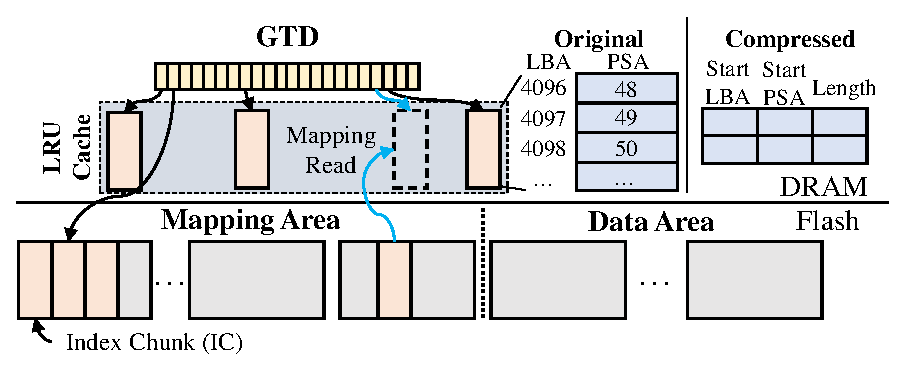
\includegraphics[width=\textwidth]{figs/OSDI/koo/dftl.eps}
         %\vspace{-5pt}
         \caption{Demand-based indexing}
         %\caption{Hybrid indexing (FAST~\cite{fast})}
         \label{fig:demand}
     \end{subfigure}
     \hfill
     \begin{subfigure}[b]{0.32\textwidth}
         \centering
         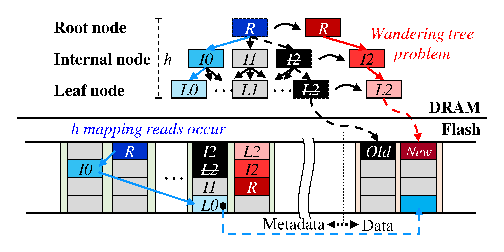
\includegraphics[width=\textwidth]{figs/OSDI/koo/uftl.eps}
         %\vspace{-5pt}
         \caption{Tree-based indexing ($\mu$-FTL~\cite{uftl})}
         \label{fig:mutree}
     \end{subfigure}
     \hfill
     \begin{subfigure}[b]{0.32\textwidth}
         \centering
         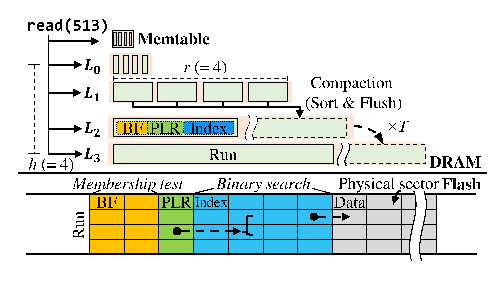
\includegraphics[width=\textwidth]{figs/OSDI/koo/lsm-short.eps}
         %\vspace{-5pt}
         \caption{LSM-tree indexing}
         \label{fig:LSM-tree}
     \end{subfigure}
    \vspace{-5pt}
	 \caption{Index structures for SSDs}
    \vspace{-20pt}
    \label{fig:ftl-review}
\label{fig:back-idx}
\end{figure*}





\begin{figure}[t]
     \centering
     \begin{subfigure}[b]{0.228\textwidth}
         \centering
         \includegraphics[width=\textwidth]{figs/OSDI/new-simul-raf.eps}
         %\vspace{-10pt}
         \caption{RAF}
        \vspace{-10pt}
     \end{subfigure}
     \hfill
     \begin{subfigure}[b]{0.24\textwidth}
         \centering
         \includegraphics[width=\textwidth]{figs/OSDI/new-simul-waf.eps}
         %\vspace{-10pt}
         \caption{WAF}
         \vspace{-10pt}
         \end{subfigure}
	 \caption{Simulation results of three index structures}
\label{fig:simul-result}
\end{figure}

\begin{comment}
\begin{figure*}[t]
\centering
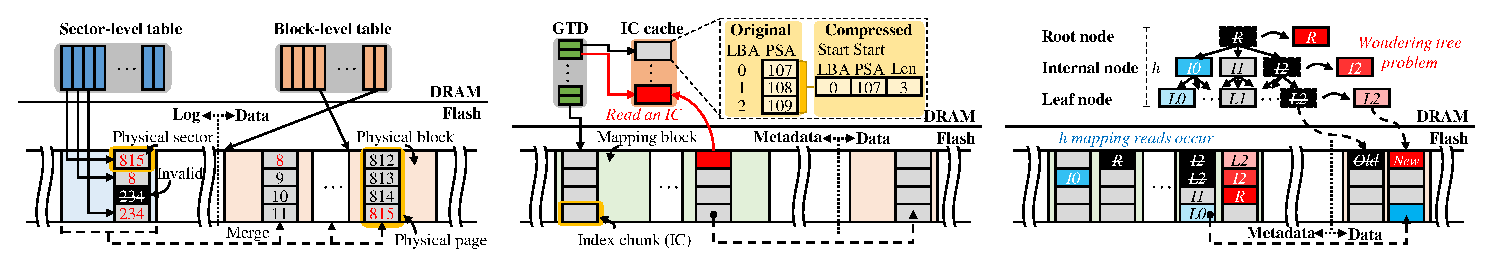
\includegraphics[height=2.85cm]{figs/OSDI/new_figs.eps}
\vspace{-3pt}
\caption{\koo{Indexing structures for SSDs}}
\label{fig:existing}
\vspace{-12pt}
\end{figure*}
\end{comment}

%-----------------------------------------------------------------------------
\section{Background and Related Work}
\label{sec:back}

We review existing index structures for SSDs 
that have been proposed over the past 20 years and 
discuss their limitations.  
%We focus on evaluating two important factors,
%a read amplification factor (RAF) and a write amplification factor (WAF),
%which represent how many \koo{\st{extra} flash} I/Os occur 
%while handling \koo{user-requested} I/Os.

\subsection{NAND Flash Basics}
\label{sec:back:table}

A NAND flash is composed of blocks, each of which consists of 128$\sim$256
pages, typically 16KB in size.  While a page is the unit of reads and
writes, a block is the unit of erasure. A 16KB page is larger than a 4KB
logical block that is the unit of I/Os in the host. Thus, four logical blocks
are stored together in the same page in a 4KB physical sector unit.  Each page
has an out-of-band (OOB) area to keep metadata (\ie~logical block
addresses) associated with the data. 

To hide the unusual property of NAND flash that does not support in-place
updates, SSD firmware, called a flash translation layer (FTL), 
appends incoming
data to free space in the flash.  
Suppose that data for a logical block address
(LBA) \LBA{i} was written to a physical sector address (PSA) \PSA{i}.
If the data for \LBA{i} is modified, its up-to-date data must be
redirected to a free physical sector address \PSA{j}.  To keep track of the
physical locations of \LBA{i}, 
the FTL maintains a sector-level L2P table in DRAM. 
The table is indexed by \LBA{i}, 
and each entry locates a sector \PSA{j} where
\LBA{i}'s data is stored.
As SSD capacity gets larger, keeping the index table entirely in DRAM becomes
difficult.  To reduce DRAM requirement, many have proposed various index
structures.

\subsection{Existing Index Structures for SSDs}
Existing index structures are categorized into three types: 
hybrid~\cite{fast,superblockFTL, last, flexibleFTL}, 
tree-based~\cite{ubifs,uftl,utree}, and demand-based
indexing~\cite{dftl,sftl,tpftl}.
We focus on evaluating two important factors,
a read amplification factor (RAF) and a write amplification factor (WAF),
which represent how many flash I/Os occur 
while handling user-requested I/Os.
\TAB{tab:raf-cost} summarizes the RAFs of the index structures.
We also conduct a simulation study using synthetic workloads with
different locality to compare RAFs and WAFs of different indexing techniques.
%understand their performance characteristics.
For the simulation, we use an SSD emulator with 512GB capacity.
A page size is 16KB and the number of pages per block is 128.
Our results are depicted in \FIG{fig:simul-result}.

\textbf{Hybrid Indexing.}
Hybrid indexing uses sector- and (flash) block-level indices to alleviate memory
pressure~\cite{fast,superblockFTL, last, flexibleFTL}.  
It splits an SSD space into log and data areas. 	
Incoming data is first written to the log area
managed by a sector-level table.
Once the log area becomes full, valid data in the log is evicted to
(or merged with) blocks in the data area.
The data area is managed by a block-level table
that uses a coarse-grained index unit and is thus memory efficient.
The log area is set small,
and most of the SSD space is used for the data area.
The hybrid indexing guarantees RAF of 1.0
(see~\TAB{tab:raf-cost}).
This is possible because
both sector- and block-level tables can entirely reside in DRAM
owing to their small sizes.
Its biggest drawback is high WAF. Moving valid data 
in the log to the data area involves many
I/Os. According to our simulation, its WAF increases up to 209.68 
(see~\FIG{fig:simul-result}).
%For this reason, the hybrid indexing is not widely used today.

\textbf{Demand-based Indexing.}
Demand-based indexing is designed to leverage locality of I/O references to
save memory.  It divides an SSD space into metadata and data areas.
The entire L2P table is kept in the metadata area, 
while the data area stores user data (see \FIG{fig:ftl-review}(a)).  
The flash-resident table is split into
fixed-size index chunks (ICs), each of which is 4KB in size.
Only popular ICs with frequently referenced entries are cached in DRAM.  The
demand-based indexing maintains a global translation directory (GTD) that keeps
track of cached or flash-resident ICs.  
Some variants like SFTL~\cite{sftl} and DFTL~\cite{tpftl} 
try to cache more entries in DRAM
by delta-encoding entries pointing to physically
consecutive sectors.

The demand-based indexing provides RAF of 1.0 on a cache hit.
But, if a cache miss occurs, it has to fetch an IC from
the flash to DRAM. It involves one extra read, increasing RAF to 2.0.
The demand-based indexing thus has RAF $= 1 + \alpha_{miss}$,
where $\alpha_{miss}$ is a cache miss ratio.
As explained in \SEC{sec:intro}, 
its performance changes greatly
by workloads and storage fragmentation that affect a cache miss ratio.
%Its RAF is highly dependent upon a cache hit ratio,
%$\alpha_{hit}$: RAF = $1 + (1-\alpha_{hit})$. 
%\JS{이후 문장들 제거?}\todo{
To make in-memory metadata persistent, 
dirty ICs and corresponding GTD entries must be
immediately or regularly flushed out to the flash, which increases its WAF. 
%To
%mitigate this problem, some or all of them are backed up by capacitors 
%within an SSD controller~\cite{spartan}.}

%However, it often suffers from severe penalties.  When the desired entry is not
%found in the cache, it must be brought into DRAM on demand, which causes an
%extra read before serving a user request.  As a result, RAF of the demand-based
%indexing varies significantly according the degree of locality.  In the worst
%case, two extra reads are required to service a single read .  
%Moreover, if a dirty IC is chosen as a victim to evict, 
%corresponding GTD entries must be flushed out to the flash, which exacerbates
%overall WAFs. To mitigate the write amplification problem,
%the GTD is usually backed up by capacitors within an SSD controller.

\textbf{Tree-based Indexing.}
Some have attempted to use trees for indexing 
(see \FIG{fig:ftl-review}(b)).  The most well-known one is
$\mu$\--FTL~\cite{uftl} that uses a variant of a B+tree, $\mu$\--tree~\cite{utree}.
%In contrast to the demand-based indexing, the tree-based indexing keeps tree
%data structures in the metadata area.  
The tree-based indexing maintains three different types of nodes: a root node,
internal nodes, and leaf nodes.  The root and internal nodes have keys and
pointers to child nodes, and leaf nodes hold indices that locate data.
All the nodes are persisted in the metadata area of the flash,
but popular nodes are cached in DRAM like the demand-based one.  
The tree-based indexing 
indexes data in a variable-sized logical chunk unit. If logically
consecutive logical blocks are stored over physically continuous sectors, 
each index points to the start location of the chunk and its length.
This is similar to what SFTL and TPFTL do in the demand-based indexing.


%The tree-based indexing has relatively low lookup complexity, $O(log(n))$, and
%has a great potential to save DRAM by indexing data in a variable-sized chunk
%unit.  
While it seems effective, the tree-based indexing has several drawbacks. 
First, it suffers from the wandering tree problem~\cite{wandering-b+}.
%First, it suffers from the wandering tree problem that deteriorates
%both WAF and RAF~\cite{todo}.  
If new data is appended to the data area, 
then an associated leaf node, internal nodes, 
and even the root node must be
updated recursively (see red nodes in \FIG{fig:ftl-review}(b)). 
The updated nodes are
eventually written to the flash, increasing WAF. 
To retrieve an index of data to read, 
it has to traverse the root and internal nodes 
along the path to reach a
leaf node (see blue nodes in \FIG{fig:ftl-review}(b)). 
This may involve several reads, increasing RAF.
Second, 
%it is vulnerable to fragmentation. 
as storage space gets fragmented, logical chunks become smaller,
which generates many nodes.
This increases a tree height $h$, resulting in more memory consumption
and higher RAF.
Finally, it still
relies on caching, suffering from the same problem as the demand-based one.
Because of the aforementioned overheads,
the tree-based indexing has RAF = $1 + h \times \alpha_{miss}$
and performs poorer than the demand-based one (see~\FIG{fig:simul-result}).

\begin{comment}
\textbf{Simulation Result.}
\FIG{fig:simul-result} shows simulation results 
of the three indexing techniques under
synthetic workloads with different locality. We emualate
a \fixme{1TB SSD} where a flash page size is 16KB and the number of pages
per block is 128. The hybrid indexing exhibits the
lowest RAF, but suffers from the extremely high WAF owing to high merge costs.
Under localized workloads, the demand-based and table-based indexing perform
better than the hybrid indexing, exhibiting both fairly low RAF and WAF.
However, they show high RAF and WAF when an input workload has weak locality or
is random.  Owing to the wandering tree problem, the tree-based indexing cannot
outperform the demand-based one.
% Please add the following required packages to your document preamble:
% \usepackage{multirow}
\end{comment}
\begin{comment}
\begin{figure}[t]
     \centering
     \begin{subfigure}[b]{0.228\textwidth}
         \centering
         \includegraphics[width=\textwidth]{figs/OSDI/new-simul-raf.eps}
         \vspace{-10pt}
         \caption{RAF}
        \vspace{-10pt}
     \end{subfigure}
     \hfill
     \begin{subfigure}[b]{0.24\textwidth}
         \centering
         \includegraphics[width=\textwidth]{figs/OSDI/new-simul-waf.eps}
         \vspace{-10pt}
         \caption{WAF}
         \vspace{-10pt}
         \end{subfigure}
	 \caption{Simulation results of three index structures}
\label{fig:simul-result}
\end{figure}
\end{comment}

\begin{comment}

\textbf{LSM-tree-based Indexing.}
There exist some index designs that use a variant of LSM-trees in SSDs
(\eg~iLSM~\cite{ilsm} and PinK~\cite{pink}).  However, their goal is to
offload a KV store engine onto an SSD to accelerate KV clients by doing KV
operations in storage.  If KV-SSDs were used as a block SSD to support typical
applications, they suffer from the same problem we mentioned above.

\end{comment}


\begin{comment}
\FIXME{
To demonstrate the inconsistent performance of demand-based FTLs, we evaluate
five FTLs in different workloads (see \SEC{sec:exp} for setup details). The
results are shown in ~\FIG{fig:motive}.  We choose the four target workloads
which are common cases that use SSDs as the storage device.  \texttt{OLTP} is
the workload generated by Filebench~\cite{filebench} that evaluates file system
performance. \texttt{FRAG-OLTP} shows the results of evaluating the same
workload as \texttt{OLTP} but, it is run under the aged file system.
\texttt{SWAP} illustrates the performance when the host system uses the SSD as
the swap memory.  We evaluate the read-only workload in YCSB~\cite{ycsb} with
the Redis KV store~\cite{redis} for \texttt{SWAP}. \texttt{CACHELIB} shows the
performance of the SSD when it is used as the main storage for cache
systems~\cite{bluedbm, kangaroo}.  The workload of \texttt{CACHELIB} is
generated by the Facebook cache engine platform~\cite{cachelib}.
}

\FIXME{
We figure out that the demand-based FTLs have large gaps among the workloads.
However, the optimal FTL shows the nearly same average read latency. The
notable results are the two SFTL performances at \texttt{OLTP} and
\texttt{FRAG-OLTP}.  Even if the average latency of \texttt{OLTP} in SFTL is
the almost same as the optimal one, the SFTL shows much poor performance under
the aged file system. It indicates that the locality of workloads would be
disturbed by the underlying systems' status. With these results, we can see
that the table-based indexing is hard to serve the consistent performance.
}
\end{comment}

\begin{comment}
\FIG{fig:dftl-exp} demonstrates the read latency of DFTL that is seriously
affected by the locality of a workload (see \SEC{sec:exp} for a more detailed
setup). Under the highly localized workload (99:1) with 100\% reads, it offers
excellent performance with almost zero cache misses.  Under the read-write
mixed (50:50) random workloads, it performs poorly owing to frequent reads to
fetch mapping entries.  Particularly, once RMW operations are involved when
serving reads, DFTL suffers from long tails.
\end{comment}




\setlength{\tabcolsep}{0.7em}
{\renewcommand{\arraystretch}{0.6}
\begin{table}[t]
\footnotesize
\centering
\caption{A comparison of RAFs of index structures}
\begin{tabular}{|l||l|l|}
\hline
\multicolumn{1}{|c||}{\textbf{Indexing technique}}    & \multicolumn{1}{c|}{\textbf{RAF}}\\ \hline \hline
Hybrid                 & $1$                    \\ \hline
Demand-based           & $1+\alpha_{miss}$    \\ \hline
Tree-based             & $1+h\times \alpha_{miss}$\\ \hline
LSM-tree               & $1+h\times r \times log_{2}(m)\times \alpha_{miss} $\\ \hline
LSM-tree+BF+PLR & {$1 +(1+(h \times r-1)\times BF_{fpr}) \times 1 \times \alpha_{miss}$} \\ \hline
\ours{}                & $1+\mathcal{E}$\\ \hline
\end{tabular}
\label{tab:raf-cost}
\vspace{5pt}
\end{table}
}


\section{LSM-tree: Opportunities and Challenges}

Existing index structures for SSDs fail to provide consistent performance,
showing skewed or highly fluctuated performance.
%Therefore, it is crucial to devise a new index structure that is able to
%provide consistent and balanced performance, regardless of workloads and
%system's condition, while consuming less DRAM.
%as  that could replace the
%existing index structures,
An LSM-tree may be considered to be a viable alternative.
An LSM-tree is a sorted multi-level search tree
where all data including metadata is always appended to the storage.  This
property is suitable for NAND flash.  

An LSM-tree is widely used to implement key-value (KV) 
stores~\cite{leveldb, rocksdb}.
Recently, there have attempts to use a variant of LSM-trees for SSDs
(\eg~iLSM~\cite{ilsm} and PinK~\cite{pink}).  
These approaches, however, aim to
offload a KV store engine onto an SSD to accelerate KV clients.  
GeckoFTL~\cite{geckoFTL} exploits an LSM-tree to mitigate 
the memory overhead of managing validity bitmaps for flash pages. 
However, it does not consider using an LSM-tree as an index structure.
To the best of
our knowledge, using an LSM-tree for indexing logical blocks to physical
sectors is not studied before.  In this section, we present how the LSM-tree
can be used for L2P indexing, presenting its opportunities and
challenges.

\begin{comment}
\begin{figure}[t]
\centering
\includegraphics[width=0.37\textwidth]{figs/OSDI/koo/lsm.eps}
\vspace{-10pt}
\caption{\fixme{LSM-tree indexing}}
\vspace{-15pt}
\label{fig:LSM-tree}
\end{figure}
\end{comment}


\subsection{LSM-tree for L2P Indexing}
\label{sec:back:lsm-tree}
%The LSM-tree is a sorted multi-level search tree that is widely to implement
%key-value (KV) stores~\cite{leveldb, rocksdb}.  
\FIG{fig:ftl-review}(c) is the organization of an LSM-tree.  An LSM-tree has
multiple levels, $L_0$, ..., $L_{h-1}$, where $h$ is a tree height.  Levels are
organized so that $L_{i+1}$ is $T$ times larger than $L_{i}$, where $T$ is a
size factor. Each level is also divided into multiple sorted runs, and each run
stores KV pairs sorted by keys over physically continuous storage space.  A run
keeps unique KV pairs, but the key range of one run may overlap with those of
other runs in any levels. The number $r$ of runs per level is the same, so a
run at $L_{i+1}$ is $T$ times larger in size than that at $L_i$.
%\FIG{fig:lsm_arch} shows the example of the LSM tree 
%when $h$=\todo{4} and $N_{run}$=\todo{4}.

In an LSM-tree, incoming KV pairs are buffered in a DRAM-resident memtable.
When the memtable is full, it sorts buffered KV pairs and appends them to a new
run at $L_0$ that resides in the storage.  KV pairs of $L_0$ are flushed out to
a run in $L_1$ when $L_0$ is full.  Similarly, once $L_i$ is full, $L_i$ is
written to $L_{i+1}$.  When flushing out $L_i$ to $L_{i+1}$, an LSM-tree
performs compaction that merges and sorts KV pairs to maintain the sorted tree.
The compaction process is simple; an LSM-tree reads in KV pairs from all the
runs at $L_i$, sorts them by key, and writes the sorted ones back to $L_{i+1}$,
creating a new sorted run at $L_{i+1}$ (see \FIG{fig:ftl-review}(c)).

An LSM-tree can be used for L2P indexing by treating an LBA
as a key and a 4KB block as a value.  For each sorted run, its metadata
is stored as a header (or a footer).  The metadata is written
together with run's data and contains L2P indices 
that point to locations of sectors for LBAs in the run.

\textbf{Opportunities.}
An LSM-tree gives us two unique opportunities.
First, an LSM-tree does not suffer from the wandering tree problem.
The change of metadata in one run does not lead 
to the updates of metadata in the other runs.
This is because of the immutability of an LSM-tree that
appends new data and metadata to the flash, 
leaving previous versions unchanged.

Second, the sorted nature of an LSM-tree makes it invulnerable
to fragmentation. Through compaction, an LSM-tree sorts
logical blocks by their LBAs and appends them 
to physically consecutive sectors. 
Each run thus has a regular pattern of <LBA,PSA> pairs,
where both LBA and PSA monotonically increase.
This property enables us to build 
memory-efficient approximate indices over the tree, without
sacrificing lookup latency.
We discuss this in detail in \SEC{sec:design:fp}--\SEC{sec:design:plr-basic}


\textbf{Challenges.}
An LSM-tree also has inherent drawbacks.  The first is high RAF.  As explained
before, tree runs have overlapped key ranges.  Given a read query (see
\texttt{read(513)} in \FIG{fig:ftl-review}(c)), starting from $L_0$, we have to look
up a run to see if it has the desired data.  If no matched entry is found, we
move on to the next run and repeat the above steps.  To serve a read query, we
have to visit up to $h \times r$ runs (\eg~16 runs in \FIG{fig:ftl-review}(c)).
Looking up each run to find desired data involves many I/Os because we have to
perform binary search over the run's metadata.  Assuming the metadata is stored
over $m$ sectors, $log_{2}(m)$ reads are needed.  Caching popular sectors of the
metadata relieves the problem, but its effectiveness depends 
on a miss ratio $\alpha_{miss}$.
Thus, the RAF of an LSM-tree can be expressed as follow: 
RAF = $1 + h \times r
\times log_{2}(m) \times \alpha_{miss}$.
As a result, an LSM-tree has much higher RAF than 
the existing index structures.

Another problem is high WAF due to compaction. As explained earlier, when
$L_{i}$ is filled with data, all the runs in $L_{i}$ must be flushed out to
$L_{i+1}$. This implies that once data is written to $L_0$, it is likely to
move from $L_0$ to $L_{h-1}$ unless it is removed or updated.  Consequently,
the WAF of an LSM-tree is proportion to $h$, WAF = $h$. Note that 
by organizing on a tree hierarchy, we can make a tree taller or fatter,
adjusting its WAF~\cite{monkey}. 
This gives us a chance to tune a tree so that 
%If a tree is organized to have
%few levels, it 
it has comparable WAF to the existing index structures
(see~\SEC{sec:design:tree}).

\subsection{Lookup Optimization}
\label{sec:back:bf}

The read amplification is a well-recognized problem in LSM-trees. To address
this, state-of-the-art LSM-trees employ Bloom filters~\cite{bloomfilter} and
piecewise linear regression~\cite{plr1,plr2,plr3}.

\textbf{Bloom Filters.}
A Bloom filter (BF) is a space-efficient data structure used to test the
existence of an item in a set~\cite{bloomfilter}. A BF is an approximate
algorithm that may return false positive results.  
An LSM-tree uses BFs~\cite{blsm, monkey, rocksdb, pebblesdb, dostoevsky} 
to avoid useless lookups on runs 
that do not have desired data.  BFs are stored as part of
run's metadata (see \FIG{fig:ftl-review}(c)), but are normally cached in DRAM for
fast lookup.  When a read comes, an LSM-tree performs membership tests
over BFs to see if desired data is stored in the run.  
If the BFs return a negative result, 
an LSM-tree moves to the next run without looking up the run.
Otherwise, it performs binary search while reading the run's metadata.
If the result turns out to be false positive, 
however, an LSM-tree keeps searching the 
tree from the next run. With BFs, $h \times r$ reduces
to $1 + (h \times r-1)\times BF_{fpr}$, where $BF_{fpr}$ is a false posive 
rate of BFs ($0<BF_{fpr}<1$) (see \TAB{tab:raf-cost}). Be advised that at least 
one run should be searched even if an LSM-tree adopts BFs.




\textbf{Piecewise Linear Regression.}
Piecewise linear regression (PLR) is a method that performs regression analysis
between independent $x$ and dependent $y$ variables. It breaks a dataset into
line segments and models each segment using a linear equation: $y=ax+b$.
PLR is used to predict the position $y_{\rho}$ of a record in a dataset, so
that $y_{\rho}$ lies within an error bound $\delta$, $|y - y_{\rho}| \leq
\delta$~\cite{plr2, plr1, plr3}.
Some recent studies~\cite{learned-index, alex-plr, bourbon} 
exploit this property 
of PLR to reduce search overheads of tree structures (\eg~{B+tree and LSM-tree}).

Bourbon~\cite{bourbon} shows that PLR is useful to make lookups
faster in LSM-trees.  
Similar to BFs, an LSM-tree stores PLR models on run's metadata, but
keeps them in DRAM for performance.  Given a read query, an LSM-tree first
estimates an approximate position of metadata in a run using PLR, and
then does binary search within a much narrower range.  
This reduces not only
lookup complexity but I/Os because only part of the metadata needs to be read.
If a metadata search range suggested by PLR 
is limited within a single sector, 
$log_{2}(m)$ reduces to 1 (see~\TAB{tab:raf-cost}).
%Rebuilding PLR models is relatively expensive.  But, the layout of the
%LSM-tree changes occasionally when compaction is triggered.  Once built,
%PLR models can be used for a long time without rebuilding.

\begin{comment}
BF and PLR are effective in reducing RAF.  With BFs, $r \times h$ reduces to
1 + ($r \times h \times BF_{fpr}$), where $BF_{fpr}$ is a false positive rate of BFs
($0<BF_{fpr}<1$).  When PLR is combined, the number of I/Os to fetch run's
metadata reduces greatly, along with lookup complexity. \polish{If a search
range suggested by PLR fits in a single sector}, $log_{2}(m)$ reduces to 1.  The
new RAF is thus as follow: RAF = $1 + ( h \times r \times BF_{fpr} \times 1) \times (1 -
\alpha_{hit})$.
\end{comment}

Through optimization with BFs and PLR, 
an LSM-tree has a reduced RAF 
= $1 + (1 + (h \times r -1) \times BF_{fpr}) \times 1 \times \alpha_{miss}$.
BFs and PLR, however, are complement data structures; run's metadata is still
needed and referenced in the read path to know a location of queried data.
The number of extra reads to fetch the metadata is decided by a
cache miss ratio.  Even worse,
an LSM-tree has to use a large BF to minimize a false positive rate.  
Similarly, to minimize approximation errors, 
we have to use a large PLR model.
While BF and PLR themselves are memory efficient, they consume non-trivial
amounts of DRAM which can be used to cache run's metadata.
This, in turn, exacerbates the memory pressure.
%As a result, even though BFs and PLR models alleviate the read
%amplification problems of LSM-trees, they exacerbate the memory pressure.






\begin{comment}
The read amplification is a well-recognized problem in LSM-trees.  
To address this,
state-of-the-art LSM-trees employ approximate techniques, bloom filters~\cite{bloomfilter} and 
piecewise linear regression~\cite{plr1,plr2,plr3}.  We explain
how LSM-trees use them to speed up read queries and present their
limitations in terms of memory usage.

\textbf{Bloom filter.}
A bloom filter (BF) is a space-efficient data structure used to test the
existence of an item in a set~\cite{bloomfilter}. A BF is an approximate
algorithm that may return \textit{false positive} results.  A BF is
organized as a $m$-bit array that is initially 0.  When a new element is
added to the set, the BF sets bit positions of the element in the $m$-bit
array using $k$ hash functions.  To query for an element in the set, the BF
computes bit positions using the same hash functions and sees if the
corresponding bits are all set to 1. If it is, the queried element \textit{may}
exist in the set. If any of the bits are 0, the element was not added before.
A false positive result occurs when a queried element has bit positions that
were set by different elements.  Given the same number of items, a
\textit{false positive rate} (FPR) of a BF is decided by (\textit{i}) the
number $k$ of hash functions and (\textit{ii}) the size $m$ of a bit array. By
increasing $k$, $m$, or both, an FPR is lowered in general, but it needs
more computation and memory. 

The LSM-tree uses BFs~\cite{blsm, monkey, rocksdb, pebblesdb} to avoid useless
lookups on runs that do not have a desired KV pair.  The LSM-tree creates BFs
for KV pairs in a run when the run is created during compaction.  The created
BFs are stored as part of the run's metadata (see \FIG{fig:lsm_arch}) but are
normally cached in DRAM for fast lookup.  When a read query comes, the LSM-tree
performs membership tests over the BFs of a target run to see if the desired KV
pair is stored in the run.  If the BFs return a negative result, the LSM-tree
moves on to the next run.  It is unnecessary to read large index tables and to
perform a binary search as the BFs guarantee that no such a KV pair exists.  If
the BFs return a positive result, it exhaustively searches the run after
reading an index table.  If it turns out be false positive, however, the LSM-tree
keeps searching the KV pair from the next run. 

\textbf{Piecewise linear regression.}
Piecewise linear regression (PLR) is a method that performs regression analysis
between independent $x$ and dependent $y$ variables. It breaks a dataset into
line segments and models each segment using a linear equation: $y=ax+b$. The
PLR is used to predict the position $y_{\rho}$ of a record in a dataset, so
that $y_{\rho}$ lies within an error bound $\delta$, $|y - y_{\rho}| \leq
\delta$~\cite{plr2}.  The PLR is known to be a memory- and compute-efficient
indexing method, particularly when a dataset has regular
patterns~\cite{bourbon,learned-index}.

Bourbon~\cite{bourbon} shows that the PLR is useful to make tree lookups faster.
Similar to BFs, the LSM-tree creates a PLR model for each run
and keeps it on the run's metadata.  PLR models are also often cached in DRAM.
Given a read query, the LSM-tree first estimates an approximate position of the
KV pair in a run using PLR models, and then does binary search within a much
narrower range.  This reduces not only lookup complexity but I/Os as only part
of the index table needs to be read.  Rebuilding PLR models is relatively expensive.
However, the layout of the LSM-tree changes occasionally only when compaction
is triggered.  Once built, PLR models can be used for a long time without
rebuilding.

Both BFs and PLR are effective in reducing the number of lookups on runs and
computation for binary search.  However, 
BFs and PLR are complement
data structures; huge index tables are still needed and referenced in the read
path to know an exact location of a queried KV pair. 
Even worse, 
to minimize a false positive rate, LSM-trees
use a large BF that needs 10-bit per KV pair~\cite{rocksdb}.  Similarly, to
minimize approximation errors of PLR models, additional 13-bit per
KV pair are needed.  While BFs and PLR are memory efficient, they
consume non-trivial amounts of DRAM. As a result, even though BFs and PLR models
alleviate the
read amplification problems of LSM-trees, they
exacerbate the memory pressure.
\end{comment}


\section{Design Principles of \ours{}}
\label{sec:overall}
\ours{} is designed to overcome the limitations of LSM-trees,
providing consistent and balanced I/O performance with minimum DRAM usage.
To achieve this goal, we develop 
\ours{} by keeping the following design principles in mind.

\begin{itemize}[leftmargin=*]
%\begin{itemize}[noitemsep,topsep=-0pt,leftmargin=*]
\item \textbf{Using Direct Indices rather than Bloom Filters.}
\ours{} does not rely on Bloom filters to decide whether to visit a specific
run or not.  Instead, it maintains a direct index table, called a
\textit{shortcut table}, which directly maps an LBA to a designated run.  The
rationale behind this decision is due to the fact that direct indices are faster
and more memory-efficient.  In our setting, a key is an integer in a specific
range (\eg~$0\sim N-1$) and its value is a 4KB block. Thus, the number of logical
blocks to be indexed is fixed. Moreover, the number of runs where
LBAs are mapped is small.  If there exist 29 runs in the tree, only 5-bit per
index is needed.  Bloom filters are useful in a situation where direct indices
cannot be used -- that is, input keys have diverse types (\eg~strings) and the
number of items to index is not fixed owing to a variable value size.  If we
construct Bloom filters using the same memory needed to build a direct table,
its false positive rate (FPR) is about 0.091. Using a direct table is reasonable, 
considering its FPR is always 0.
%the number of unnecessary visits
%to runs becomes 0, that is $1 + (r \times h \times BF_{fpr})$ reduces to 1.
%small. By using a shortcut table, $r$$\times$$h$ becomes 1.

%\item \textbf{Principle \#2 -- No exact indices}:
\item \textbf{Guessing rather than Caching}.
%An LSM-tree keeps exact indices in its metadata which \textit{exactly} point to
%physical sectors for logical blocks and, for performance, it caches some of
%them.  For this reason, 
An LSM-tree caches popular metadata of runs in DRAM,
so its performance is highly dependent upon a cache miss
ratio.  
\ours{} takes a different approach; it only uses approximate indices to
\textit{guess} locations of data in runs over its read path.  Compared to exact indices
that need 32-bit per entry (for 16TB SSDs), approximate indices require
3.8$\sim$7.86-bit per entry.  This space efficiency makes it possible
to keep entire
indices in DRAM without relying on caching.  Approximate indices inevitably
result in errors that may involve extra I/Os.
%Resolving such errors may involve lots of I/Os.
%\ours{} address this problem by exploiting the property of approximate algorithms
%that guarantees a target error rate. 
%Taking an example of
%one specific design point, \ours{} ensures the error rate of 0.1 (\ie~one 
%error out of 10 queries) while achieving 3.43$\times$ memory efficiency.
However, if an error rate $\mathcal{E}$ is controlled sufficiently low,
approximation is a better choice.  
The performance of caching is affected by
various factors we cannot control, such as I/O locality and fragmentation.
On the other hand, only the factor that decides the performance of
approximation is an error rate 
which can be preset at the design time.  This
enables us to provide consistent I/O latency, regardless of input workloads and
system's condition.

%which cause extra reads while servicing user I/Os. The key technical issue is
%thus how to accurately estimate a physical location of an input query.  an
%input query while assigning minimal DRAM to approximate algorithms. To this To
%this end, \ours{} employs a \textit{tiered indexing structure} that combines
%exact indexing, BFs, and PLR models at different tree levels.  at different
%tree levels in a manner that minimize both error rates and memory usage.  Our
%indexing structure is Motivated by the fact that BFs and PLR models enable us
%to set a specific error rate, trading accuracy against memory usage, we
%carefully design BFs and PLRs to guarantee a target error rate with minimal
%DRAM usage. 

\begin{comment}
Our goal is to use approximate algorithms to eliminate the \textit{necessity}
of index tables in its read path.  \ours{} employs only two lightweight
approximate data structures, BFs and PLR models, in DRAM and uses them to
locate a physical sector of data to access.  No index tables are needed to find
a location of data. By keeping only memory-efficient data structures in the
memory, \ours{} can greatly reduce the amount of DRAM for the address
translation.

The approximate indexing of \ours{} inevitably results in trial errors which
cause extra reads while servicing user I/Os. The key technical issue is thus
how to accurately estimate a physical location of an input query.
%an input query while assigning minimal DRAM to approximate algorithms. To this
%To this end, \ours{} employs a \textit{tiered indexing structure} that
%combines exact indexing, BFs, and PLR models at different tree levels.  at
%different tree levels in a manner that minimize both error rates and memory
%usage.  Our indexing structure is 
Motivated by the fact that BFs and PLR models enable us to set a specific error
rate, trading accuracy against memory usage, we carefully design BFs and PLRs
to guarantee a target error rate with minimal DRAM usage. Taking an example of
one specific design point, \ours{} ensures the error rate of 0.1 (\ie~one error
out of 10 queries) while consuming 3.43$\times$ less DRAM than typical FTL
designs.
\end{comment}

%\item \textbf{Principle \#3 -- No caching}:
\item \textbf{Balancing Tree for Balanced Performance.}
The WAF of an LSM-tree is decided 
by adjusting a tree height $h$ as pointed out in \SEC{sec:back:lsm-tree}.
However, reorganizing a tree hierarchy also has impacts on RAF and memory consumption.
%As explained in \SEC{todo}, we are able to adjust write throughput by
%adjusting the height of the tree. Reorganizing the tree, however, has
%an impact on memory usages and RAF. 
While taking into account such impacts,
we carefully adjust the organization of a tree
for \ours{} to provide reasonable WAF.
\ours{} provides similar or slightly higher WAFs
than the existing index structures. This does not
diminish the value of \ours{}. Prioritizing reads is reasonable
as they have a higher impact on user-perceived
performance. On the other hand, write throughput can be optimized in various
ways, for example, write buffering~\cite{write-buffer}.
\end{itemize}

\begin{comment}
\ours{} adjusts the organization of a tree to provide reasonable WAF.
%reduces WAF of the tree by adjusting the organization of a tree, offering a 
%sufficiently low WAF (see~\SEC{todo}). 
Moreover, by combining SSD's cleaning and compaction and by optimizing compaction process
to minimize amount of data to migrate, \ours{} further reduces 
WAF. Depending on workloads, \ours{} provides similar or slightly higher WAFs
than the existing index structures. This does not
diminish the value of \ours{}. Optimizing reads first is reasonable
because they have a higher impact on user-perceived
performance. Write throughput can also be optimized in various
ways via write buffering~\cite{write-buffer}, 
write suspension/resume~\cite{suspension}, and
so on.
\end{comment}

In summary, \ours{} eliminates unnecessary visits to runs 
by using direct indices rather than Bloom filters. 
Instead of caching metadata,
\ours{} loads entire approximate indices in DRAM.
By doing so, in \ours{}, $BF_{fpr}$ becomes zero,
and a cache miss rate, $\alpha_{miss}$, is replaced with an approximation 
error rate, $\mathcal{E}$. As a result,
\ours{} has RAF = 1 + $\mathcal{E}$ ($0 < \mathcal{E} < 1.0$).
Unless otherwise stated, our target $\mathcal{E}$ is set to 0.1.
It means that \ours{} guarantees RAF of 1.1, which is close
to that of when an entire L2P table is loaded in DRAM.

\begin{comment}
First, high RAF caused by looking up runs in the tree never occur
in \ours{}. Instead, by looking up the shortcut table, \ours{} is able to 
visit a target run without extra reads.
Moreover, since all the indices are kept in the memory entirely,
\ours{} is not 
affected by various factors we cannot control, such as temporal and spatial
locality of workloads and system conditions (\ie~fragmentation).
%that provide quite diverse performance depending on given workloads
On the contrary, the read latency of \ours{} is only decided by a preset error
rate. Even under random I/O workloads running over severely fragmented space,
the error rate of \ours{} is maintained at a target level. This property of
\ours{} enables us to guarantee the expected performance all the time,
regardless of input workloads and system conditions.
\end{comment}

\begin{comment}
\begin{itemize}[leftmargin=*]
\item \textbf{Principle \#4 -- Balancing the tree for balanced WAF}:
High WAF caused by compaction is another drawback of the LSM-tree.  \ours{}
reduces WAF of the tree by adjusting the organization of a tree, offering a 
offering a sufficiently low WAF (see~\SEC{todo}). Moreover,
by combining FTL's GC and compaction and by optimizing compaction process
to minimize amount of data to migrate, \ours{} achieves comparable 
WAF to other index structures. This does not
diminish the value of \ours{} as reads have a higher impact on user-perceived
performance. Write throughput of SSDs can also be optimized in various
ways via write buffering~\cite{write-buffer}, 
write suspension/resume~\cite{suspension}, and
so on.
\end{itemize}
\end{comment}

\begin{comment}
\subsection{Basic Idea} 
Typical LSM-trees using approximate algorithms aim to reduce the
\textit{probability} of looking up exact indices in index tables. Our goal is
to use approximate algorithms to eliminate the \textit{necessity} of index
tables in its read path.
\ours{} employs only two lightweight approximate data structures, BFs and PLR
models, in DRAM and uses them to locate a physical sector of data to access. 
No index tables are needed to find a location of data. By keeping only
memory-efficient data structures in the memory, \ours{} can greatly reduce the
amount of DRAM for the address translation.
%DRAM and uses them to guess a physical location of data to access.  In this
%way, \ours{} enables to load the entire data structures in smaller DRAM
%(5$\times$ smaller than the typical FTL), avoiding costly I/Os to retrieve
%exact indices while serving user requests.

The approximate indexing of \ours{} inevitably results in trial errors which
cause extra reads while servicing user I/Os. The key technical issue is thus
how to accurately estimate a physical location of an input query.
%an input query while assigning minimal DRAM to approximate algorithms. To this
%To this end, \ours{} employs a \textit{tiered indexing structure} that
%combines exact indexing, BFs, and PLR models at different tree levels.  at
%different tree levels in a manner that minimize both error rates and memory
%usage.  Our indexing structure is 
Motivated by the fact that BFs and PLR models enable us to set a specific error
rate, trading accuracy against memory usage, we carefully design BFs and PLRs
to guarantee a target error rate with minimal DRAM usage. Taking an example of
one specific design point, \ours{} ensures the error rate of 0.1 (\ie~one 
error out of 10 queries) while consuming 3.43$\times$ less DRAM than typical FTL
designs.

Yet another important benefit of \ours{} that it can provide consistent
latency. The read latency of existing FTL designs varies greatly and is
affected by various factors we cannot control, such as temporal and spatial
locality of workloads and system conditions (\ie~fragmentation).
%that provide quite diverse performance depending on given workloads
On the contrary, the read latency of \ours{} is only decided by a preset error
rate. Even under random I/O workloads running over severely fragmented space,
the error rate of \ours{} is maintained at a target level. This property of
\ours{} enables us to guarantee the expected performance all the time,
regardless of input workloads and system conditions.

In the following sections, we first explain the overall design of \ours{},
along with its operations (\SEC{design:overall}). Then, we present how our
approximate algorithms work (\SEC{sec:design:bf-plr-basic}).
%how \ours{} manages the LSM tree and handle basic I/O operations. Then, we
%present how \ours{} (나머지 쓰고 나중에 쓰자...)}
\end{comment}



%-----------------------------------------------------------------------------
%\section{Design of \ours{}}
\begin{figure}[t]
\centering
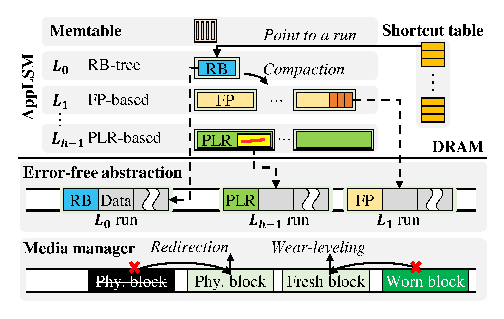
\includegraphics[width=0.37\textwidth]{figs/OSDI/koo/overall.eps}
\caption{Overall architecture of \ours{}}
\label{fig:overall}
\end{figure}

\section{Design and Implementation of \ours{}} 
\label{sec:new-design}
%This section describes the overall design of \ours{} and the techniques to
%reduce DRAM, flash writes, and reads.
\ours{} can be implemented in an OS kernel or in an SSD controller.
For typical SSDs that expose overwriteable logical blocks to the
host, \ours{} is implemented in an SSD controller as the form of firmware.
For latest ZNS SSDs~\cite{zns-ssd} and OCSSDs~\cite{ocssd} that expose
append-only media~\cite{dm-zoned}, \ours{} runs in OS's kernel
(\eg~\texttt{dm-zap}~\cite{dm-zap}), performing L2P indexing on the host
side.  For the sake of presentation, we assume that \ours{} is implemented in
an SSD controller.

In this section, we first explain the overall design of \ours{}, along with its
operations (\SEC{design:overall}). Then, we present how our approximate
algorithms work (\SEC{sec:design:fp}--\SEC{sec:design:plr-basic}).
Finally, we explain how \ours{} can be organized to provide reasonable WAFs
with minimal memory usages (\SEC{sec:combine}--\SEC{sec:design:tree}).


\subsection{Overall Organization} 
\label{design:overall}
%We explain key components that comprise \ours{} and associated data structures.
%Then, we present how \ours{} handles read and write requests.

%\textbf{System Components.}
\FIG{fig:overall} illustrates the overall organization of \ours{}
with its key components.
A \textit{media manager} is responsible for managing error-prone NAND
chips. It provides error-free NAND abstraction -- physical blocks 
and pages -- to upper-level components by internally performing bad-block 
management and  wear-leveling with a tiny redirection table. 

%NAND chips are shipped with bad blocks. As NAND blocks are erased repeatedly,
%moreover, they gradually wear out and become bad blocks.  Regardless of which
%index structure is used, SSD firmware should be able to manage error-prone NAND
%ㅈchips.  In \ours{}, a \textit{media manager} is responsible for managing NAND
%chips, providing error-free NAND abstraction (\ie~pages and blocks) to
%upper-level components.  For managing bad blocks and wear-leveling, it
%maintains a tiny redirection table that maps flash blocks (exposed to the upper
%layers) to NAND-device blocks.  Once a bad block is identified, the media
%manager excludes it by updating  the redirection table. It also internally
%performs wear-leveling for balanced block wearing. 
\begin{comment}
NAND chips are shipped with bad blocks. As NAND blocks are erased repeatedly,
moreover, they gradually wear out and become bad blocks.  Regardless of which
index structure is used, SSD firmware should be able to manage error-prone NAND
chips.  In \ours{}, a \textit{media manager} is responsible for managing NAND
chips, providing error-free NAND abstraction (\ie~pages and blocks) to
upper-level components.  For managing bad blocks and wear-leveling, it
maintains a tiny redirection table that maps flash blocks (exposed to the upper
layers) to NAND-device blocks.  Once a bad block is identified, the media
manager excludes it by updating  the redirection table. It also internally
performs wear-leveling for balanced block wearing. 
\end{comment}

Over the error-free NAND abstraction, 
\ours{} organizes its flash-resident data structures.
Individual runs are stored over physically continuous flash blocks (exposed by
the media manager). Each run is divided into metadata and data areas.
The metadata area keeps indices pointing to data in the data area
and is stored at the beginning of each run when
run's data is written to the flash.  
Flash-resident metadata is never used to locate data in the read path.  
It is only used for reconstructing its in-memory data
structures after system reboots.

\ours{} has four in-memory data structures: a \textit{memtable}, a
\textit{shortcut table}, and two types of \textit{approximate indices}.  
The memtable is equivalent to a write buffer. Its size is several MBs
(\eg~1MB$\sim$4MB) in size, and it is large enough to fully utilize write
throughput of NAND devices. The shortcut table is referenced to find a run that
has data to access.  It is an LBA-indexed flat table, each entry of which
points to a run where a logical block is stored.  \ours{} usually maintains 29
runs in the tree, so 5-bit per entry is enough to locate all possible runs.
For individual runs, \ours{} maintains approximate indices, 
in-memory copies of run's metadata. 
Two different algorithms, \textit{fingerprint} (FP)- and
\textit{PLR-based approximation}, are used to build approximate
indices. Each run chooses one that requires less memory.

%The shortcut table is more memory efficient than typical bloom filters.  When
%we build bloom filters using the same amount of memory, it suffers from an FPR
%of 0.091, but the shortcut table ensures an FPR of 0.0.  Be advised that the
%shortcut table is applicable only a key is an integer and the maximum number
%of items to store is determined when designing the system like \ours{}.

%When a write request comes, \ours{} buffers its data in a memtable that is
%equivalent to a write buffer in an SSD. Like conventional SSDs, the memtable
%is several MBs (\eg~1MB$\sim$4MB) in size, but is large enough to fully
%utilize write throughput of NAND devices.

\textbf{I/O Operations.}
We explain how \ours{} handles write requests.  Incoming logical blocks
are first buffered in the memtable.  Once it becomes full, \ours{} flushes out
pending data to $L_0$.  \ours{} manages $L_0$ as a log,
appending pending data to $L_0$ without sorting through compaction.  This
approach is useful to remove I/O overheads caused by frequent compaction
between the memtable and $L_0$~\cite{rocksdb,leveldb}.  For fast query over $L_0$, \ours{}
maintains a \textit{red-black (RB) tree}.  
The RB-tree is tiny as $L_0$ is small in size. 

Once $L_i$ is filled with data, \ours{} flushes out 
the data of all runs in $L_i$ to a new run in $L_{i+1}$
via compaction. 
%It is necessary to keep the tree sorted. 
%When writing data to a new run in $L_{i+1}$,
During compaction, 
\ours{} builds approximate indices and writes them to the metadata area 
of the new run.
Corresponding entries in the shortcut table must be updated 
accordingly to point to the new run.
In our design, compaction substitutes SSD's cleaning process
as the overall procedures of the two are almost the same; 
they read data from runs
(or victim blocks) and move them to a new run (or free space). 
The only difference is that \ours{} needs to sort data by LBA.  
\ours{} reduces compaction I/Os by excluding outdated data.
Existing LSM-trees move all data to a new run, including obsolete ones,
because of high tree lookup costs. On the other hand,
\ours{} can quickly identify whether a run has the latest version of 
data or not by referring to the shortcut table.

%Another difference is that, while
%SSD cleaning excludes outdated data (which were overwritten by new data),
%LSM-tree moves all the data in runs to a new run, including obsolete ones.
%This is because high lookup cost. To identify outdated data, it has to look up
%the tree. \ours{} can easily identify obsolete data by referring to the shortcut
%table, lowering compaction costs.


%Except that the compaction needs to sort data by keys, the overall procedures of
%LSM-tree's compaction and FTL's GC are identical; they read data from runs (or
%victim blocks), exclude invalid ones, and write them to free space. 
%\koo{However, for the lowest level $L_{h-1}$, the compaction of \ours{} performs differently
%from that of LSM-trees. In LSM-trees,
%there is no limit in the height of the tree.
%Thus, once the last level $L_{h-1}$ becomes full, they create a new last level $L_{h}$
%and move data to it. 기존 LSM-tree도 h가 시작 시에 정해져 있고, 마지막 레벨은 AppLSM과 비슷한 방식 아닌지 확인 필요.}
%On the other hand, \ours{} limits the tree height to $h-1$ as
%the creation of a new level requires additional DRAM to maintain indices.
%Instead, within the last level $L_{h-1}$,
%\ours{} repeats moving data in a victim run to a free run,
%filtering out invalid ones. 
%This is similar to what typical FTLs do for GC. 




\begin{comment}
\textbf{Data Structure.}
Once the memtable becomes full, \ours{} flushes out pending data to $L_0$. In
our design, $L_0$ has a single run. The run size is one of the configurable
parameters, and it usually ranges from 5MB to 5.4GB for a 1TB SSD. 
Since the 
run is larger than the memtable, \ours{} performs costly merge-sort operations
to maintain the sorted run in $L_0$, whenever the memtable is flushed out to
$L_0$.
%\cancel{\ours{} reads in data from $L_0$, merge-sorts them with those
%in the memtable, and finally writes them back to $L_0$.}  
To avoid costly
merge-sort operations, \ours{} manages $L_0$ as a log, appending data to
$L_0$ all the time. For fast query, \ours{} maintains exact indices for $L_0$
that hold <$x_i$, $y_i$> pairs sorted by $x_i$. $L_0$ is small in size, so DRAM
for the exact indices is tiny (\eg~10.8MB when the run size is
5.4GB). It is worth noting that some KV stores
employ the same approach to lessen flush overheads~\cite{rocksdb}.
\end{comment}

\begin{comment}
\textbf{Operations.}
%Besides $L_0$, the rest of levels $L_1$, ..., $L_{h-1}$ are managed in the same
The rest of levels $L_1$, ..., $L_{h-1}$ are managed in the same
manner as explained in \SEC{sec:back:lsm-tree}. Once $L_i$ is filled with data,
\ours{} flushes data from $L_i$ to $L_{i+1}$ through compaction to keep the
tree sorted.  The compaction is costly since it involves many I/Os,
increasing a write amplification factor (WAF) = 
($\frac{\text{data written to flash}}{\text{data written by host}}$).
\ours{}
reduces the number of I/Os for the compaction by adjusting the organization of a tree
(see \SEC{sec:design:tree}),
%\sout{and applying several optimization techniques (see \SEC{todo})}.
offering a sufficiently low WAF. However, the
resulting WAF is still higher than those of typical FTLs. This does not
diminish the value of \ours{} as reads have a higher impact on user-perceived
performance. Write throughput of SSDs can also be optimized in various
ways via write buffering~\cite{write-buffer}, 
write suspension/resume~\cite{suspension}, and
so on.
\end{comment}

%\ours{} handles a read query differently from typical LSM-trees.  
Given an LBA to query, \ours{} looks up the shortcut table
and finds a designated run that has a physical sector for the LBA.
Then, \ours{} searches for desired data in the run.
Each run is managed by different indexing strategies.
%\ours{} uses different indexing strategies for levels.  
If the run belongs to the $L_0$, 
\ours{} retrieves wanted data
by looking up the RB-tree.
%Through binary search, \ours{} can find an exact location of the given query.  
For the other levels that are managed by either FP- or PLR-based
indexing, \ours{} estimates the
location of the given LBA by following the approximate algorithm
and reads data from the suggested location.
If the location holds wrong data, 
\ours{} has to perform a local search
or moves to the next run to find the correct one.  
%A prediction error incurs extra I/Os.
%\JS{\sout{As such errors repeat, 
%the performance of \ours{} degrades significantly.}}

Prediction errors involve unnecessary I/Os.
Thus, a primary issue in designing \ours{} is how to
provide a low error rate while consuming as less memory as possible.
We discuss these issues in \SEC{sec:design:fp}--\SEC{sec:design:plr-basic}.
Besides accuracy and memory efficiency, 
we also present how we make index lookup faster,
which is another important design factor.

\subsection{FP-based Approximate Indexing}
\label{sec:design:fp}

%\subsubsection{FP-based indexing}
%\label{sec:design:fp-basic}

Let us first explain how \ours{} manages a run in a tree using FP-based
indexing.  For each run $R_i$, logical blocks $x_i$ sorted by their LBAs are stored in
physically consecutive sectors $y_i$.  To map logical blocks $x_i$ to physical
sectors $y_i$, $R_i$ maintains a set of $<x_i,y_i>$ pairs in the memory: $R_i =
\{<x_0,y_0>,<x_{1},y_{1}>, ..., <x_{n-1},y_{n-1}>\}$, where $n$ is the number
of logical blocks (or sectors) in a run.  In \ours{}, $y_i$ increases by 1
monotonically, and thus it only needs to keep $x_i$ in $R_i$. Therefore,
$R_i$ can be rewritten as follows: $R_i = \{x_0,x_{1}, ..., x_{n-1}\}$.
Here, $x_i$ is a large integer number (\eg~32-bit for 16TB SSD) and 
increases as an SSD capacity grows. The FP-based indexing aims to reduce
the memory requirement by replacing $x_i$ with short fingerprints $FP_i$:
$R_i^{FP} = \{FP_0,FP_{1}, ..., FP_{n-1}\}$.

\begin{figure}[t]
\centering
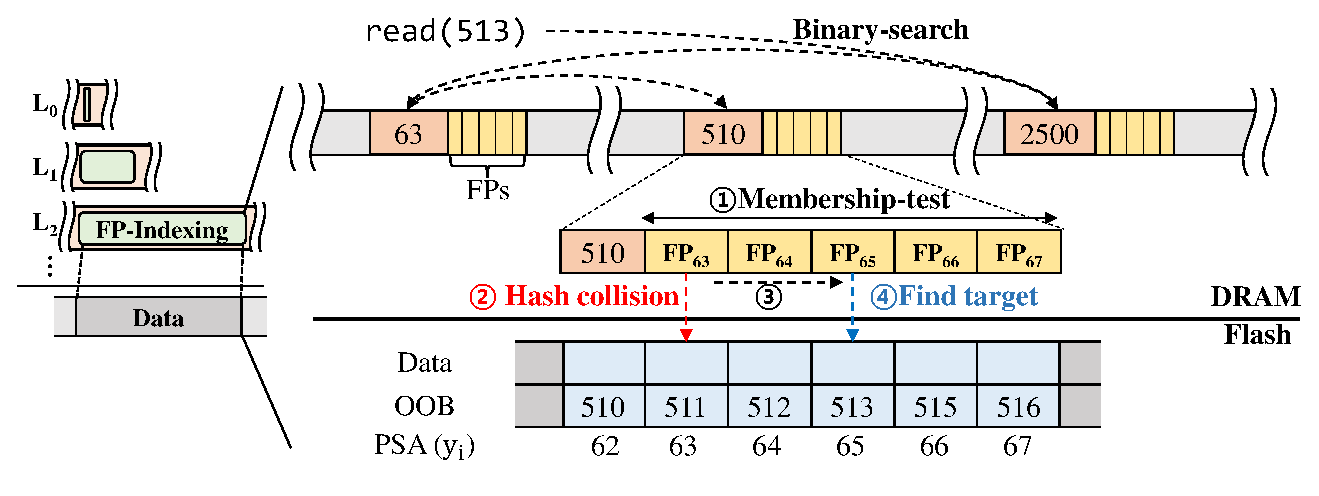
\includegraphics[width=0.45\textwidth]{figs/OSDI/FP.eps}
\caption{FP-based approximate indexing and its operations}

\label{fig:overall:fp}
\end{figure}


\FIG{fig:overall:fp} depicts the organization of an FP-based index table.
FP indices are organized similar to those in an
inverted page table; (\textit{i}) each entry holds \FP{i} of $x_i$ rather
than $y_i$ and (\textit{ii}) the position of an entry in the table specifies
its location in the run. The construction of the FP table is straightforward.
When logical blocks are flushed out to a new run during compaction, 
\ours{} records their $FP_{i}$ in the in-memory table (the same copy is stored in
the metadata as well).
In the example of \FIG{fig:overall:fp}, data for \LBA{i} = 511 is written to
\PSA{i} = 63.  \FP{i} is set to hold \textit{hash}(511) of \LBA{i}.  While
writing data to \PSA{i}, its exact LBA, 511, is written to \PSA{i}'s OOB.

Handling a read request is more complicated.  When a read query for \LBA{j} = 513
comes, \ours{} has to examine FPs in the table {(\wcircled{1})}.  Starting
from the first FP, \ours{} compares \textit{hash}(\LBA{j}) with
\FP{i} until it finds the matched one.  Each run holds many FP indices,
so it may take considerable time.  To
mitigate this problem, \ours{} splits the FP table into smaller FP groups with $k$ FPs.  
The first entry of each FP group holds an exact (but large) LBA number, while the
rest hold short FPs.  In this way, \ours{} can perform binary
search over encoded FPs, choosing a narrower range of FPs to examine. 
The lookup complexity is thus $O$($log_{2}\frac{n}{k}+k$).
%\JS{\sout{As will
%be discussed later, an FP group fits in a 64B CPU cache line, enabling us
%to quickly compare FPs with few bitwise operations (see \SEC{sec:design:bf-lookup}).}}

A hash collision inevitably occurs while comparing FPs.
%\ours{} inevitably suffers from collision false positive results. 
Taking the example of \FIG{fig:overall:fp}, \FP{63} has the same value of 
\textit{hash}(513). \ours{} reads a physical sector \PSA{63},
but can identify that \PSA{63} has data for LBA 511 by referring 
to \PSA{63}'s OOB. Since \PSA{63} has wrong data {(\wcircled{2})},  \ours{}
ignores \PSA{63} and continues the tests on the remaining FPs (\wcircled{3}).
Once it finds the correct one, it finishes the test (\wcircled{4}).

Hash collisions incur extra I/Os.  For \ours{} to outperform the existing
index structures, given the same amount of DRAM, it must
provide a low
collision rate, so that the number of extra I/Os by collision errors 
is smaller than that by cache misses. 
In the next subsection, we
theoretically analyze an error rate of the FP-based indexing and show that \ours{} 
exhibits smaller memory footprints than the existing index structures
while ensuring a fairly low error rate.

\subsubsection{Memory Optimization}

Let $C$ be a collision rate of \FP{i}.  As each \FP{i} has more bits (consumes
more memory), it exhibits lower $C$, and vice versa.  Given $C$, 
the number |\FP{i}| of bits needed for \FP{i} can be easily obtained using 
the equation $|\FP{i}| = \ceil{log_{2}\frac{1}{C}}$.

Let $\mathcal{E}_{FP}$ be an error rate of the FP-indexing.
$\mathcal{E}_{FP}$
represents a rate at which hash collisions (\ie~errors) happen
while serving one read request in an FP group. Each FP group is assumed to have $k$ FPs.  
If $\mathcal{E}_{FP}$ is 0.1, it means that one hash collision occurs while serving 10
read requests.
In our design,
one hash collision results in one extra read, and thus
$\mathcal{E}_{FP}$
can be directly translated to RAF (\ie~$\mathcal{E}_{FP}$ of 0.1 = RAF of 1.1).

\begin{comment}
Let's assume that each FP group has $k$ physical sectors. \ours{} maintains
the same number of FPs in the group. A hash collision rate $HCR$ of each FP
is inversely proportion to the number of bits it has. That is, as an FP has more bits,
it exhibits a low $HCR$.
Given a target FPR, $FPR_{T}$, to achieve,
we estimate how many bits each FP needs. 
$FPR_{T}$ represents how many hash collisions occur while searching for data in the FP table.
%is a rate at which one read query to an FP group suffers from
%false positive answers.
$FPR_{T}$ can be set any number between $0 < FPR_{T} < 1$,
but for now, $FPR_{T}$ is
assumed to be 0.1 (\ie{}~one hash collision occurs while serving 10 queries), 
\end{comment}

We define a sequence $Req$ of read requests for $x_i$ in an FP group: $Req =
<$\LBA{0}, ..., \LBA{k-1}$>$ where \LBA{i} is issued before \LBA{j} if $i<j$.
For the sake of simplicity, the number $|Req|$ of requests is the same as
the number of physical sectors in an FP group (\ie~$|Req| = k$).  To assume a random
workload, each LBA is issued only once (\ie~\LBA{0} $\neq$ \LBA{1}
$\neq$ ... $\neq$ \LBA{k-1}), and \LBA{0}, ..., \LBA{k-1} are stored reversely
from the last sector to the first one.
%\koo{from \fixme{\PSA{k-1}, ..., \PSA{0} in the run} 보다는 the last sector of the run. 대체 고려. 이전까지는 \PSA{k-1}은 \LBA{k-1}이 저장된 PSA 인데, 이 문장에서는 Run의 마지막 PSA로 되어있음. 변경 필요.}

For \LBA{0} in $Req$, we have to look up all the FPs fr
om \FP{0} to \FP{k-1}
because \LBA{0} is stored in the last sector of the run.
%because \LBA{0} is stored in \koo{\fixme{\PSA{k-1}} 이것을 the last sector of the run}.
The error rate for \LBA{0} is thus $1 - (1 - C)^{k-1}$.
Similarly, for \LBA{1}, we need to check \FP{0}, ...,
\FP{k-2}, and its error rate is $1 - (1 - C)^{k-2}$. Finally,
for \LBA{k-1}, no collision happens. In this way, 
$\mathcal{E}_{FP}$ to serve all requests in $Req$ 
is estimated as follows:
% \begin{equation}
% 	\small
% \begin{split}
% 	\small
% 	\mathcal{E}_{FP}	= \ & \frac{1}{k} \cdot \sum^{k}_{i=1}{(1 - (1 - C)^{k-i})} = \ 1 - \frac{1-(1-C)^{k}}{k \cdot C}.
% \end{split}
% \label{eq:fpr-relax}
% \end{equation}

\noindent\small
\begin{align}\label{eq:fpr-relax}
 	\mathcal{E}_{FP}	= \ & \frac{1}{k} \cdot \sum^{k}_{i=1}{(1 - (1 - C)^{k-i})} = \ 1 - \frac{1-(1-C)^{k}}{k \cdot C}.
\end{align}
\normalsize



\begin{comment}
\begin{figure}[t]
     \centering
     \begin{subfigure}[b]{0.23\textwidth}
         \centering
         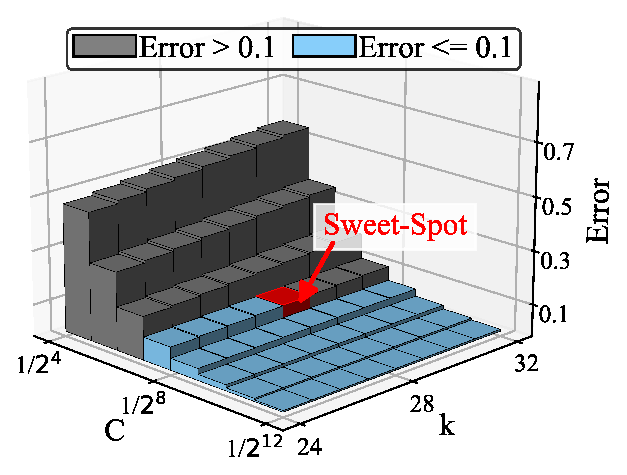
\includegraphics[width=\textwidth]{figs/OSDI/3d-fpr.eps}
         \caption{Error rate}
         \label{fig:hybrid}
     \end{subfigure}
     \hfill
     \begin{subfigure}[b]{0.23\textwidth}
         \centering
         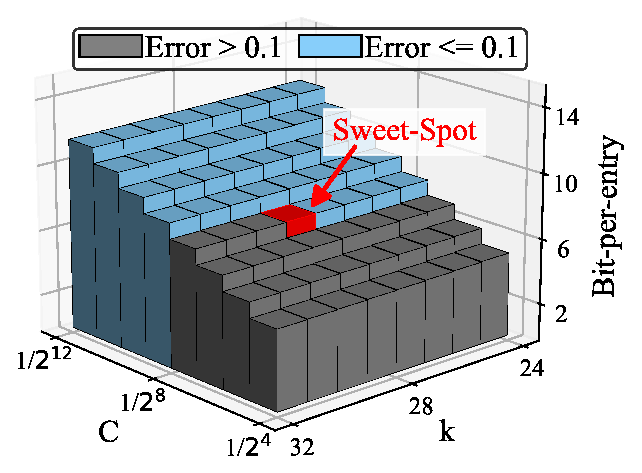
\includegraphics[width=\textwidth]{figs/OSDI/3d-bit.eps}
         \caption{Bit-per-entry}
         \label{fig:demand}
     \end{subfigure}
	 \vspace{-10pt}
	 \caption{\fixme{$\mathcal{E}_{FP}$ and memory requirements under varying C and k}}
	 \vspace{-10pt}
\label{fig:fp-CK}
\end{figure}

\FIG{fig:fp-CK} plots $\mathcal{E}_{FP}$ and
the number of bits per FP table entry (memory requirements) 
depending on $C$ and $k$. 
As expected, as $C$ gets lower, $\mathcal{E}_{FP}$ becomes smaller, but more
memory is needed.  Similarly, $\mathcal{E}_{FP}$
decreases as $k$ gets smaller. 
%This also results in high memory consumption. 
However, with smaller $k$,
\ours{} maintains a large number of small FP groups in the run.
Thus, the memory consumed by exact LBAs becomes significant,
which, in turn, increases bits per table entry.
\end{comment}

Eq.~(\ref{eq:fpr-relax}) tells us that $\mathcal{E}_{FP}$ is decided by
two variables $C$ and $k$. 
If our target error rate $\mathcal{E}_{FP}$ is 0.1, 
the best combination of <$C$, $k$>,
which requires the minimum memory,
is <0.0079, 28>. Using $|\FP{i}| = \ceil{log_{2}\frac{1}{C}}$,
each FP needs 7 bits to satisfy $C$ of 0.0079.
Since each FG group has 27 FP indices plus a 32-bit exact index,
the average size of the table entry is 7.89 bits.
Compared to typical exact indexing with 32-bit entries, \ours{} achieves 4.05$\times$ memory efficiency.
\begin{comment}
28개 일 경우 0.0079, 7, 27, (27*7+32)/32
29개 일 경우 0.
\end{comment}
%Even more, while exact indexing requires more bits to index data as an SSD capacity
%grows, \ours{} needs to increase an exact index. This means that \ours{} is a more scalable solution.

\begin{comment}
Eq.~(\ref{eq:fpr-relax}) cannot be solved for $FPR_{BF}$ using linear algebra.
However, it is clear that, for the same target FPR, $FPR_{BF}$ inbegin
Eq.~(\ref{eq:fpr-relax}) is higher than that in Eq.~(\ref{eq:fpr}).  If
$FPR_{T}^{R}$ is 0.1 and $n$=512, $FPR_{BF}$ from Eq.~(\ref{eq:fpr-relax}) is
4.2$\times$10$^{-4}$, which is higher than
2.06$\times$10$^{-4}$.  {The higher $FPR_{BF}$, the smaller $BF_i$} as
more false positive errors can be tolerated by \ours{}.  As a result, the relaxed BF needs
22-bit for each \BF{i}.
\FIXME{
가드를 고려하지 않고 수식을 정리했다는 언급이 필요함
}
\FIXME{
(n=512 --> $FPR_{BF}=0.00042065$ changed from 0.00041982, bit=12)
(n=28 --> $FPR_{BF}=0.00822996$, bit=7)
}
\end{comment}



\subsubsection{Lookup Optimization}
\label{sec:design:bf-lookup}

As discussed before, \ours{} has $O$($log\frac{n}{k}+k$) time to
look up an FP table.
To minimize lookup latency, we layout FPs in the memory to align with the
cache line boundary. Each FP group has 27 7-bit FPs, plus one exact index.
A 64B CPU cache line is large enough to accommodate two FP groups.
We split the cache line into two partitions -- 32B or 256-bit each -- and
place an FP group (221-bit) on each.  We increase $k$ from 27
to 32 so that each group fits in a 256-bit partition.  
It slightly increases the error rate $\mathcal{E}_{FP}$ (from 0.092 to 0.11), 
but we can better utilize the available memory.  
This memory layout also gets rid of extra memory references
caused by the miss-alignment.  
Moreover, since all the FPs are packed within a 64B integer,
comparing candidate FPs with an input LBA can be done at once
with few bit-wise operations.




%Looking up the table requires two steps: binary search and membership tests.
%The binary search over guards requires $O$($log~k$) time, where $k$ is the
%number of guards in the table.  The membership tests on candidate BFs between
%two guards require $O$(n) time. 
%As a result, \ours{} has
%logarithmic time complexity $O$($log~k+n$) for tree lookup. Thus, the
%majority of actual lookup time is spent on the membership test.  

%We minimize lookup latency by layouting BFs in the memory to align with the
%cache line boundary. Each guard embraces 28 7-bit BFs.
%The 64B CPU cache line is large enough to accommodate two guards and 56 BFs.
%Thus, we split the cache line into two partitions -- 32B or 256-bit each -- and
%place a guard and its BFs (228-bit in total) on each.  We increase $n$ from 28
%to 32 so that a guard plus its BFs fit in a 256-bit partition.  Even though it
%slightly increases the FPR (from 0.096 to 0.11), we can maximally
%utilize the available memory.  This memory layout also enables us to prefetch
%candidate BFs while performing binary search without any extra memory
%references.  Moreover, since all the BFs are packed within a 64B integer,
%comparing candidate BFs to an input LBA can be done at once
%with few bit-wise operations.



%The BF-based indexing is simple but gives us a huge benefit.  DFTL issues extra
%reads to fetch mapping entries from the flash when a cache miss happens.  In
%\ours{}, unnecessary reads occur only when BFs return false positive answers.
%However, 
%For \ours{} to outperform the demand-based FTLs, it should provide an acceptable
%FPR that is lower than a miss rate of them, while consuming less DRAM than
%the demand-based ones.  
%\ours{} also requires to perform binary search and scanning over BFs,
%which may cause lots of computation.  
%In \SEC{sec:opt:memory}, we explain various optimization techniques 
%to improve the accuracy of the BF-based indexing at low  
%memory usage and fast lookup latency in detail.
%Through various optimizations, \ours{}
%reduces the number of bits per BF to \JS{7.86} and provide the BF lookup
%latency of 0.55 $\mu$s.  The detailed explanation of the optimization is given
%in \SEC{sec:opt:memory}.

%In the worst case, all the BFs in a run should be examined (see
%\SEC{sec:opt:latency}).  We explain how these issues are addressed.







\subsection{PLR-based Approximate Indexing}
\label{sec:design:plr-basic}

To further reduce the memory usage, \ours{} takes a more aggressive approach
using PLR which has a potential to
express many entries <$x_i$, $y_i$> using a few linear equations. 

Given $R_i$ = \{<$x_0$, $y_0$>, <$x_1$, $y_1$>, ..., <$x_{n-1}$, $y_{n-1}$>\},
\ours{} transforms $R_i$ into a set of line segments 
$R_i^{PLR}$ = \{$S_0$, $S_1$, ..., $S_{k-1}$\} using PLR.
Each line segment $S_h$ is modeled by a linear equation, $y_i'=a_h(x_i-x_h)+b_h+y_h$, 
where $a_h$ is a slope, $b_h$ is an intercept, and $x_h$ and $y_h$ are
the first x-y coordinate of $S_h$ in the run.
It approximates the physical location $y_i$ of $x_i$.
A predicted location $y_i'$ is within a bounded error $\delta$.
That is, $y_i'$ is guaranteed to lie within [\PSA{i} - $\delta$, \PSA{i} + $\delta$).

\begin{figure}[t]
\centering
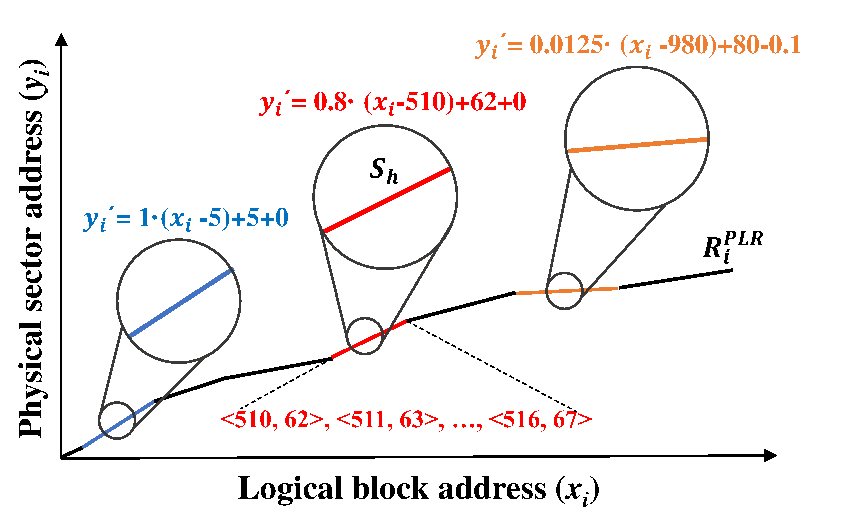
\includegraphics[width=0.34\textwidth]{figs/OSDI/PLR_org.eps}

\caption{Examples of PLR-based approximate indexing}
\label{fig:plr_base}
\vspace{-5pt}
\end{figure}

Similar to the FP-based indexing, \ours{} creates a PLR-indexed table for a new run
that is being created during compaction, and its copy is stored in the flash as
part of the run's metadata.  A PLR table keeps parameters of linear
equations: $a_h$, $b_h$, $x_h$, and $y_h$ for $S_{h}$.
\FIG{fig:plr_base} shows the example of how \ours{} converts $R_i$ = \{...,
<510, 62>, <511, 63>, ..., <516, 67>, ...\} into $R_i^{PLR}$ = \{..., $S_h$,
...\}, where $S_h$ is expressed as the linear equation
$y_i'=0.8\cdot(x_i-510)+62$.

To retrieve data for \LBA{i}, \ours{} finds a designated run using the shortcut table
and then performs binary search to find a PLR model by looking up x-coordinates
in a PLR table. Taking the example of \FIG{fig:overall:plr} where \LBA{i} =
515 comes to query, the model returns $y_i'=66$ and $\delta$ is 0 since $y_i=66$. 
\ours{} also suffers from a prediction error. If $x_j=513$, the predicted
$y_j'=64.4$ with $\delta$ of 0.6.  To resolve an error, extra I/Os are
unavoidable.  In the following subsection, we explain how \ours{} controls an
error rate $\mathcal{E}_{PLR}$ of the PLR-based indexing and applies it to PLR
models.
%This may lead to extra I/Os to resolve an error.
%Similar to the FP-based indexing, we design the PLR-based indexing
%so that it guarantees a target error rate, trading 
%DRAM usage.  
%Looking up and building PLR models should be performed
%efficiently as well.  

%To achieve the above goals, we refactor the original PLR
%algorithm (OptimalPLR~\cite{plr3}) that has a general-purpose design for any
%applications. By refactoring it suitable for \ours{}, we can express a linear
%equation using fewer bits without sacrificing prediction accuracy too much.  We
%also minimize user-perceived performance penalties by building PLR models while
%performing compaction I/Os.  A detailed explanation is given in
%\SEC{sec:design:plr}.
\begin{figure}[b]
\centering
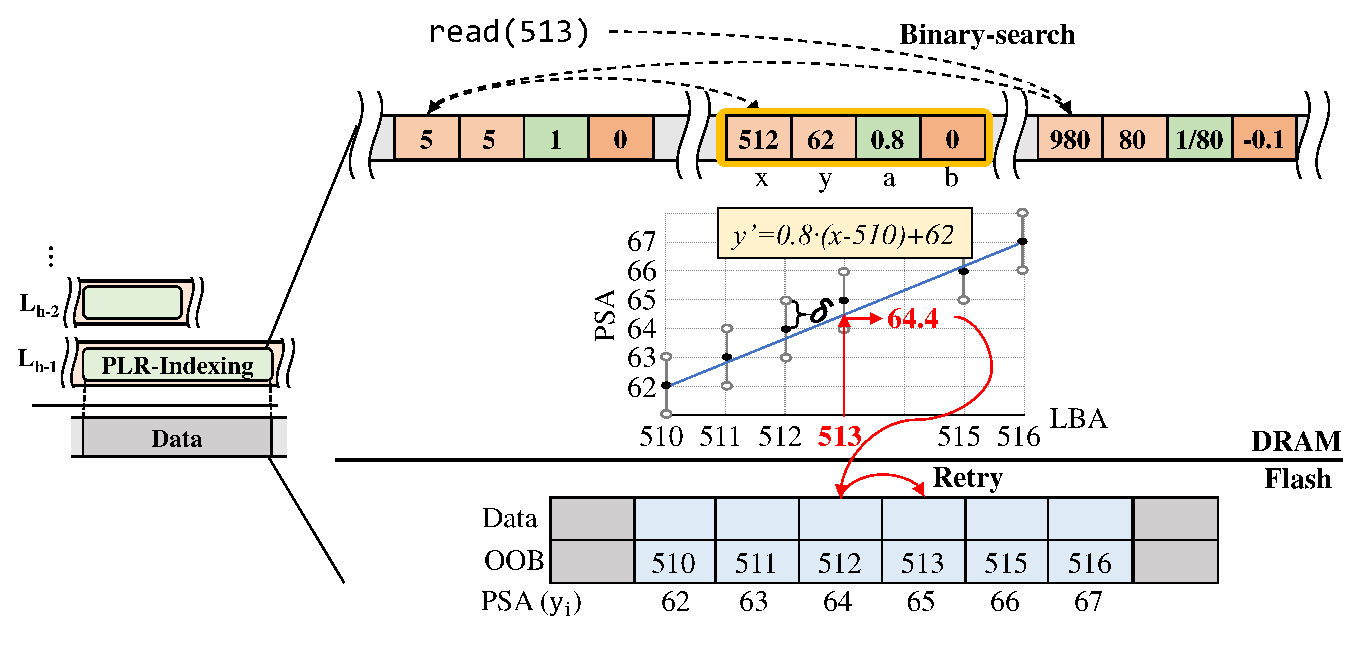
\includegraphics[width=0.45\textwidth]{figs/OSDI/PLR.eps}
\vspace{-5pt}
\caption{PLR-based approximate indexing and its operations}

\label{fig:overall:plr}
\end{figure}

\subsubsection{PLR Error Rate Control}
\begin{figure}[t]
\centering
%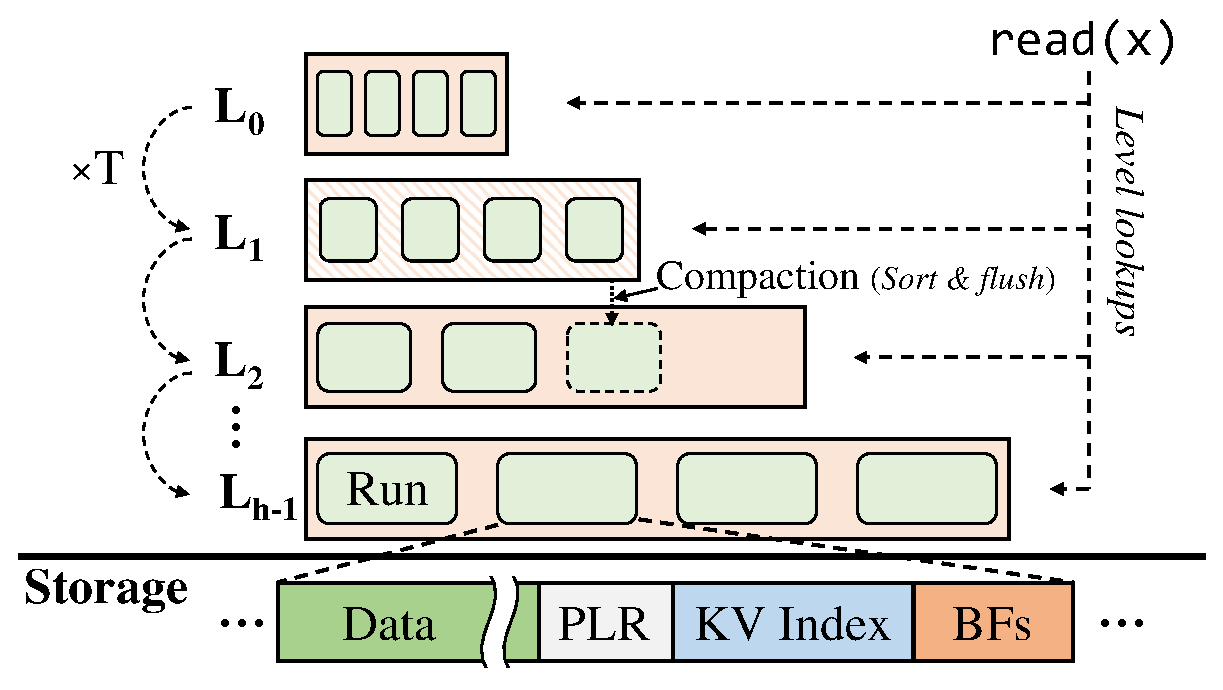
\includegraphics[height=3.3cm]{fig2.eps}
\includegraphics[height=2.5cm]{figs/OSDI/plr-ctr.eps}
\caption{Error control in PLR}
\label{fig:plr-control}
\vspace{-5pt}
\end{figure}

Let us first take a look at the
organization of NAND flash in \FIG{fig:plr-control}, where 
4KB logical blocks, $x_{i}$, $x_{i+1}$, $x_{i+2}$, and $x_{i+3}$
are stored in four consecutive 4KB sectors, $y_{i}$,
$y_{i+1}$, $y_{i+2}$, and $y_{i+3}$.
The four sectors belong to the same NAND page.
Since a page is the unit of I/O in the flash, the logical blocks (or physical sectors) are
read together. 

In \FIG{fig:plr-control}, assuming that $\delta$ is set to 1.5 when building the
PLR model, so that the error of the predicted $y_i'$ is less than 1.5.
Under a fully random workload, when serving a read request to $x_{i}$, the
probability of requiring more than one page read is 33\%
(\ie~$\mathcal{E}_{PLR}$ of 0.33).  If $-0.5 \leq y_i'-y_i < 1.5$, one 16KB page
read is sufficient to service $x_{i}$ without any trial errors.  Only when
$-1.5 \leq y_i'-y_i < -0.5$, a neighboring page is read unnecessarily.  For
$x_{i+1}$, $x_{i+2}$, and $x_{i+3}$, their $\mathcal{E}_{PLR}$s are estimated as
0, 0, and 0.33, respectively. As a result, the average $\mathcal{E}_{PLR}$
is 0.167 when $\delta$ is 1.5.

By reducing $\delta$, we can make $\mathcal{E}_{PLR}$ smaller.  If
$\delta = 0.83$, $\mathcal{E}_{PLR}$ of 0.1 is ensured.  However, setting
$\delta$ so tightly ($\delta$ = 0.1) comes at the cost of more memory
usage.  This is because the PLR algorithm has to create more line
segments in $R_{PLR}$, so as not to violate a narrow range of $\delta$.  
If $\delta$ is too large (\eg~$\delta = 10$), 
PLR creates $R_i^{PLR}$ with fewer segments but suffers from many errors. 
Developing a new PLR
algorithm that creates a smaller number of line segments with tight $\delta$
is beyond our scope.  Instead, we aim to reduce memory
requirement of line segments through system-level optimizations.

%because each line segment is able to cover many
%mapping pairs without violation of the designated $\delta$. 

%We may further reduce extra I/Os caused by errors by 

%Reducing $\delta$ further may lower extra I/Os caused by errors.  However, this
%comes at the cost of more memory.  Given the same input $R_i$.  the PLR
%algorithm needs to create more line segments if $\delta$ is set so tightly.
%Conversely, if $\delta$ is too large (\eg~$\delta=0.5$), the PLR creates
%$R_i^{PLR}$ with fewer segments because each line segment is able to cover many
%mapping pairs without violation of the designated $\delta$. \FIG{todo} displays
%the number of line segments needed to cover the same $R_i$ depending on
%$\delta$.
    

\begin{comment}
\begin{figure}[t]
\centering
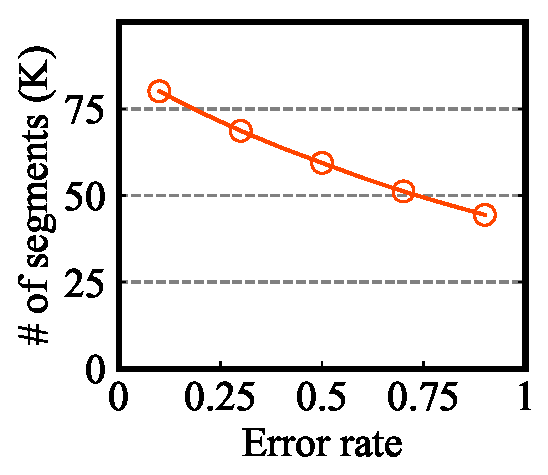
\includegraphics[height=3cm]{figs/OSDI/PLR-Error.eps}
\vspace{-10pt}
\caption{\FIXME{Number of line segments under varying error rates}}
\vspace{-10pt}
\label{fig:plr-error-memory}
\end{figure}

{
\renewcommand{\arraystretch}{0.4}
\begin{table}[t]
    \small
    \caption{Bits-per-line-segment (BPL) after PLR optimization}
    \vspace{-10pt}
    \centering
    \begin{tabular}{|c||c|c|c|c|}
        \hline
                                 &  {Unoptimized}  & {+Slope}  & {+Intercept}  & {+Delta}  \\
                                & {PLR} & {quantization} & {quantization} & {encoding}\\\hline
    BPL	    &  256-bit     &    203-bit     & 151-bit      &46.2-bit   \\ \hline
    \end{tabular}
    \label{tab:plr-opt}
    \vspace{-10pt}
\end{table}
}
\end{comment}

\subsubsection{Memory Optimization}

The PLR itself is memory efficient, but there exists room to further
improve its memory efficiency.  
To model a various range of $<x_i, y_i>$ pairs supplied as an input,
the original PLR uses real numbers, 8B each, for four components of a linear equation. 
Each line segment thus needs 32B in total, which dwarfs its
memory efficiency.  
%The original PLR provides higher
%memory efficiency than exact indexing, but cannot outperform the BF-based
%indexing (see \FIG{fig:tree-org}(a) in \SEC{sec:design:tree}).
%Fortunately, unlike typical use cases of PLR where 
%a various range of $<x_i, y_i>$ pairs are provided as an input,
\ours{} has quite regular $<x_i, y_i>$ patterns within each run,
thanks to the property of an LSM-tree.
%thanks to the sorted nature of the LSM-tree.
%In \ours{}, $x_i$ increases monotonically all the time 
%(\ie~$x_i < x_j$ if $i < j$) because of sorted nature of the LSM-tree.
%Moreover, $y_i$ always increases by 1 since all the incoming data
%is appended to the run.
By leveraging such properties, \ours{} applies (\textit{i}) quantization and
(\textit{ii}) delta-encoding to reduce the sizes of four line parameters,
$a_h$, $b_h$, $x_h$, and $y_h$.
%It enables us to construct memory-efficient PLR models without sacrificing
%accuracy too much.
%Table~\ref{tab:plr-opt} summarizes
%the number of bits per line segment after applying
%optimization techniques to the PLR-based indexing.
%through quantizing and compressing the components.
%\ours{} leverages such properties to construct memory-efficient models.
%\todo{(최적화 기법들에 대한 간단한 언급???)}




\begin{comment}
\begin{figure}[t]
    \centering
    \begin{subfigure}[b]{0.17\textwidth}
         \centering
         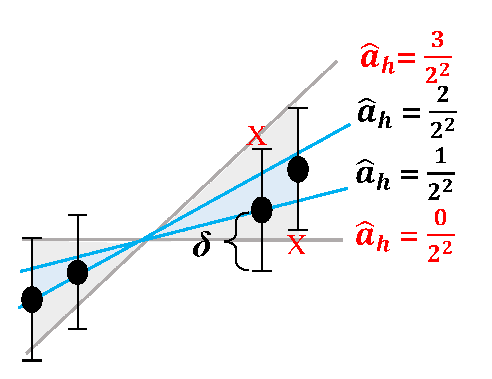
\includegraphics[width=\textwidth]{figs/OSDI/slope_quant.eps}
         \vspace{-10pt}
         \caption{Slope quantization}
         \vspace{-10pt}
    \end{subfigure}
    \hfill
     \begin{subfigure}[b]{0.15\textwidth}
         \centering
         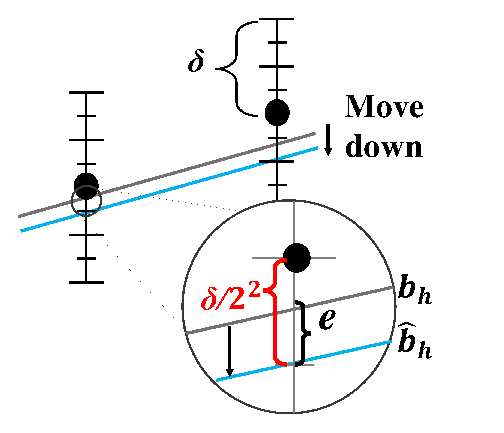
\includegraphics[width=\textwidth]{figs/OSDI/inter-quant.eps}
         \vspace{-10pt}
         \caption{Intercept quantization}
         \vspace{-10pt}
    \end{subfigure}
    \caption{Slope and intercept quantization ($t=2$)}
\label{fig:plr_opt}	 
\end{figure}
\end{comment}
\textbf{Slope Quantization.} 
Typical PLR algorithms consider a broad range of possible slopes $\rho$
($-\infty<\rho<\infty$) to create a smaller
number of line segments.  \ours{} can
create almost the same number of line segments as that of typical PLRs even if a range of $\rho$ is
limited to $0 < \rho \leq 1$ because of the following two properties.

First, the highest slope of the line segment that \ours{} has is at most 1.0.
This extreme case occurs where both $x_i$ and $y_i$ increase
monotonically by 1, for example, $R_i$ = \{<5, 5>, <6, 6>, ...,
<20, 20>\} (see the first segment in \FIG{fig:plr_base}). Second, the lowest
slope in \ours{} is at least higher than 0.0. This happens when $x_i$ increases
much faster than $y_i$, for example, $R_i$ = \{<980, 80>, <1060, 81>, <1139,82>,
..., <3380, 110>\} (see the third segment in \FIG{fig:plr_base}).
%Therefore, even if \ours{} models a given $<x_i, y_i>$ pairs with
%possible slope $0 \leq \rho \leq 1$, it can find a sufficiently small number of
%line segments.

This narrow slope range makes it easier that $a_h$ is expressed by
fewer bits.  \ours{} uses only $t$-bit to express $a_h$ by
quantizing a slope range into $2^t$
discrete finite ones ($\frac{0}{2^t}$, $\frac{1}{2^t}$, ...,
$\frac{2^t-1}{2^t}$) as shown in \FIG{fig:plr_opt}(a). 
The quantized version $\hat a_h$ of $a_h$
is defined as $\hat a_h = \Delta \cdot \floor*{\frac{a_h}{\Delta}}$, 
where the step size $\Delta$ is $\frac{1}{2^t}$.
Owing to quantization errors,
we may not create a line segment even if there exist possible
slopes expressed by an 8B real number.
%Consider $t=2$ where $\hat a_{(i,j)}$ can express 0.0, 0.25,
%0.5, and 0.75 slopes.  
%Suppose $t=2$ and $\hat a_{(i,j)}$ can be 0.0, 0.25,
%0.5, or 0.75. If a feasible slope range $\rho$ lies between 0.6 and 
%0.7, no line segments can be created. 
This results in more
line segments, which in turn leads to memory waste.  
But, when $t$ = 11, the number of line
segments generated is similar to that of 
OptimalPLR~\cite{plr3}, an optimal PLR algorithm generating
the minimal number of segments.

\begin{figure}[t]
\centering
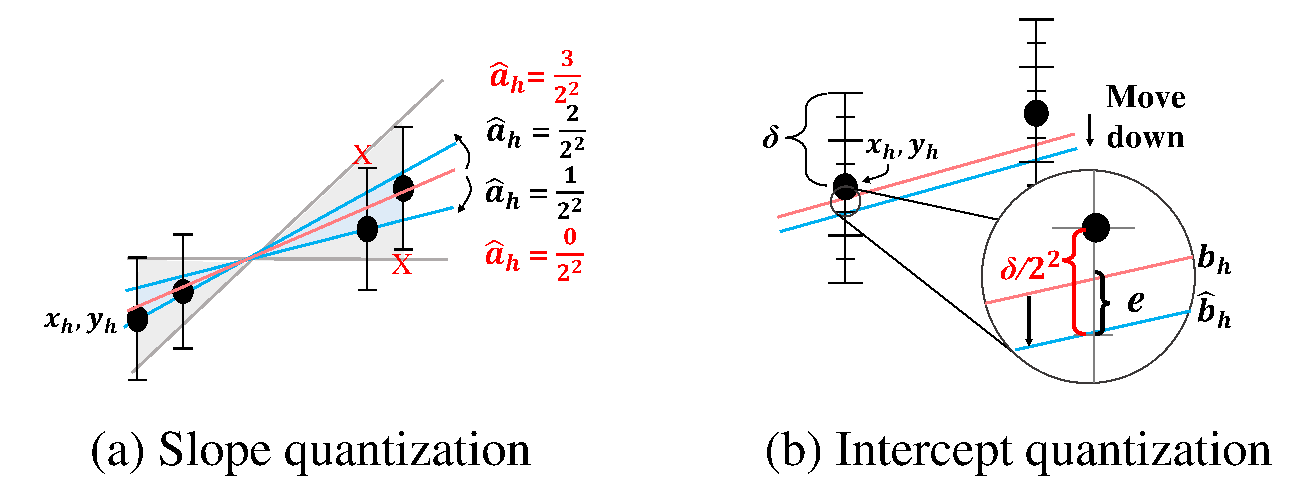
\includegraphics[width=0.43\textwidth]{figs/OSDI/PLR_opt_2.eps}
\caption{Slope and intercept quantization ($t=2$)}
\label{fig:plr_opt}
\end{figure}

\textbf{Intercept Quantization.}
Since the number of possible slopes is limited to $2^t$, possible intercepts
$b_h$ on the y-axis are also limited.  To take advantage of this
property, we quantize $b_h$, expressing it using a finite discrete
number. 
For any feasible line segment, $b_h$ must be in the range $-\delta\leq
b_h\leq\delta$. \ours{} uniformly divides the possible range $2 \cdot
\delta$ of $b_h$ into $2^{t+1}$ quantized levels with the step size
$\Delta = \frac{\delta}{2^t}$.  Thus, only $t+1$-bit is needed to represent a
quantized intercept.  The quantized version $\hat b_h$ of $b_h$
is expressed as $\hat b_h = \Delta \cdot \floor*{\frac{b_h}{\Delta}}$.  

With the intercept quantization, the original line segment
vertically moves down (see \FIG{fig:plr_opt}(b)) 
since the floor function is used to quantize $b_h$.
Owing to the error, the quantized line segment may violate the condition 
$|y'_i-y_i|\leq\delta$.
This also results in more line segments, wasting memory.
Currently, we use the same $t=11$ for the intercept
quantization which is large enough. The violation rarely happens in
practice.  

\textbf{Delta-encoding.}
To express the first x-y coordinate $x_h$ and $y_h$ of $S_h$,
\ours{} uses two 4B integers.
To further reduce their sizes, \ours{} employs delta-encoding.  
Given two consecutive
line segments $S_h$ and $S_{h+1}$, \ours{} only keeps 
deltas $x_{h+1} - x_{h}$ and $y_{h+1} - y_h$ for $S_{h+1}$, instead of
$x_{h+1}$ and $y_{h+1}$.
The delta-encoding effectively saves memory requirement.
However, to find a line segment that contains a specific $x_i$, we have
to scan the PLR-indexed table while performing delta-decoding.  
To mitigate the overhead, we take the similar approach used in the FP-indexed table.
\ours{} splits the PLR-indexed table into multiple PLR groups
and maintains uncompressed $x_h$ and $y_h$ at the beginning of each group.
%for every $d$ fragment, \ours{} maintains a pivot pair that keeps uncompressed
%$x_i$ and $y_i$.  
In this way, 
\ours{} can quickly find a wanted PLR group via binary-search 
and retrieve a desired line segment by scanning a smaller number of candidates.
The time complexity 
is $O(log_{2}\frac{f}{d}+d)$, where $f$ is the number of line segments in a run
and $d$ is the number of line segments in a group.

\subsubsection{Lookup Optimization}
To balance the lookup latency against memory consumption,
we also apply the similar optimization as we did for the FP-indexed table
when deciding the size of each PLR group.
For delta-compressed x-y coordinates,
we assign 11-bit and 9-bit, respectively.
For every PLR group, we should maintain uncompressed $x_h$ and $y_h$,
each of which requires a 4B integer (if the SSD capacity is 16TB).
Since $a_h$ and $b_h$ need 11-bit and 12-bit, respectively, 
we can pack one uncompressed segment (87-bit) and 
9 compressed segments (43-bit each), 10 segments in total,
into a 64B CPU cache line. Considering that 
the original PLR requires 256-bit per segment, \ours{} achieves 5$\times$ memory efficiency to express a line segment.


\begin{comment}
The memory space required for $m_{(i,j)}$ in a run is 
$f \cdot \{\mathcal{C}(x_i)+\mathcal{C}(y_i)\}$, where $\mathcal{C}(x_i)$ and
$\mathcal{C}(y_i)$ are the numbers of bits required for delta-encoded $x_i$
and $y_i$.  Currently,
$\mathcal{C}(x_i)$ and $\mathcal{C}(y_i)$ are 11-bit and 9-bit,
respectively.  For (uncompressed) pivot pairs, \ours{} still needs two 4B
integers, along with a 4B index that points to the start
location of compressed fragments to scan.  The memory consumption of pivot
pairs is $\frac{f}{d} \cdot (4 + 4 + 4)$\ bytes.
If $d$ is 30, for every 30 fragments, a 12B pivot pair is needed.
The memory overhead per each fragment is thus 3.2-bit.

In summary, for the four parameters of the linear equation, the original PLR
needs 256-bit ($= 64 + 64 + 64 + 64$).  
\ours{} reduces it to 46.2-bit ($= 11 + 12 + 11 + 9 +  3.2$) where $t
= 11$, $\mathcal{C}(x_i) = 11$, 
$\mathcal{C}(y_i) = 9$ and the pivot overhead per fragment is $3.2$.
If the number $f$ of fragments is the same as the two, 
we achieve 5.5$\times$ memory
efficiency over the original PLR.
\end{comment}


\begin{comment}
\subsubsection{PLR Model Creation}

We first formally explain how \ours{} creates PLR models using an example in
\FIG{fig:plr-indexing}.  Let $M = \{m_1, m_2, ..., m_n\}$ be a set of mapping
pairs $m_i = (x_i, y_i)$ in a run.  We use $m_{(i, j)} = \{m_i, m_{i+1}, ...,
m_j\}$ $(1\leq i < j \leq n)$ to denote a set fragment.  
%Given $M$ and a target error bound $\delta$, \ours{} divides $M$ into set
%fragments, so that each fragment $m_{(i, j)}$ is represented by a line segment
%whose linear function $y_h' = a \cdot x_h +b$ satisfies $|y_h' - y_h| \leq
%\delta$ for any pair $m_h = (x_h, y_h)$ in $m_{(i,j)}$.
Given $M$ and a target error bound $\delta$, \ours{} divides $M$ into set
fragments so that each fragment $m_{(i, j)}$ is modeled by a line segment
whose linear equation $y_h' = a \cdot x_h +b$ satisfies $|y_h' - y_h| \leq
\delta$ for any pair $m_h = (x_h, y_h)$ in $m_{(i,j)}$.  \ours{} maintains
multiple set fragments for $M$.  Thus, the linear equation of the line segment
for $m_{(i, j)}$ is defined as follows:
\begin{equation}
\small
\begin{split}
	y_h' = a_{(i, j)} \cdot (x_h - x_i) + y_i + b_{(i, j)},
\end{split}
\label{eq:linear}
\end{equation}
%where $x_i$ and $y_i$ are from the first pair $m_i$ and used as a base
%point where $m_{(i, j)}$ starts.  
where $x_i$ and $y_i$ are coordinates where $m_{(i, j)}$ starts.  $a_{(i, j)}$
is the slope of the line segment for $m_{(i, j)}$, and $b_{(i, j)}$ is the
relative intercept of the line from \PSA{i}.  
In \FIG{fig:plr-indexing} where seven pairs $m_1=(2,1)$, ..., $m_7=(46,7)$ are
given, there are two line segments for $m_{(1,4)}$ and $m_{(5,7)}$. $m_1=(2,1)$
and $m_5=(43,5)$ are start coordinates. For $m_{(1,4)}$, $a_{(1,4)}=0.6$ and
$b_{(1,4)}=0$, and for $m_{(5,7)}$, $a_{(5,7)}=0.33$ and $b_{(5,7)}=0.5$.


Four parameters, $a_{(i, j)}$, $b_{(i, j)}$, $x_i$, and $y_i$, are kept in
DRAM.  Thus, it is important to construct a small number of line segments 
to save memory. \ours{} uses OptimalPLR~\cite{plr3} to find an
optimally minimal number of line segments. OptimalPLR is designed 
for online streams and thus is fast.
We explain how \ours{} creates line segments using OptimalPLR below.

\begin{figure}[t]
\centering
%\includegraphics[height=5.3cm]{test.eps}
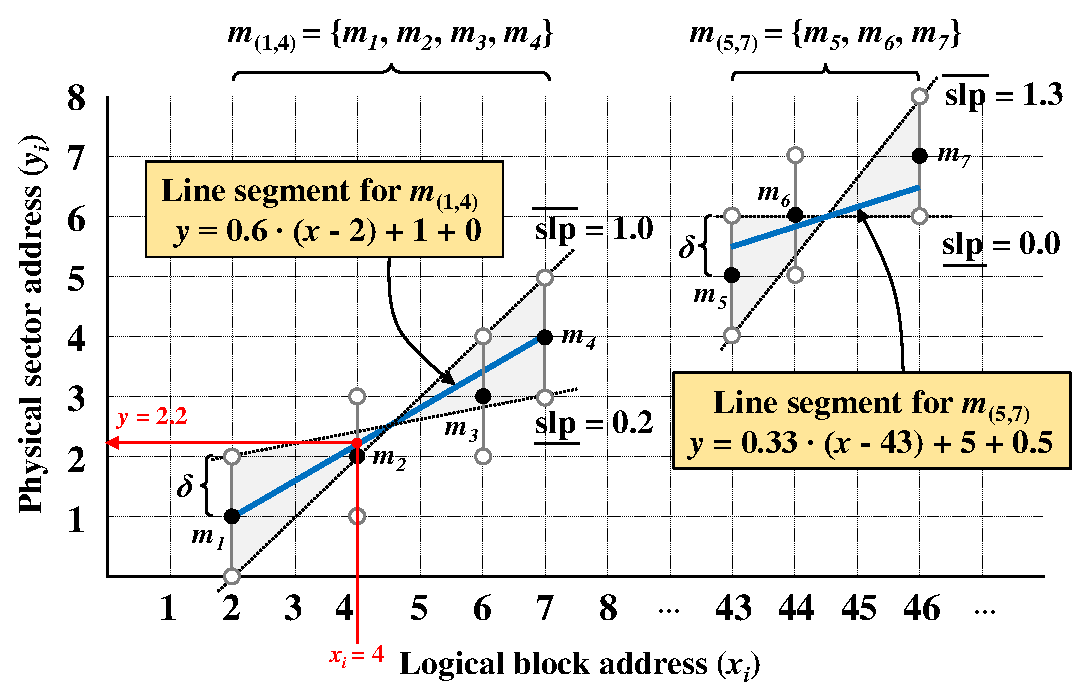
\includegraphics[height=5cm]{./figs/figs-final/fig-plr.eps}
\vspace{-10pt}
\caption{Examples of PLR-based approximate indexing}
\vspace{-10pt}
\label{fig:plr-indexing}
\end{figure}

Initially, \ours{} starts with no set fragments. Given $M$, it creates an empty set
fragment and adds a mapping pair from $M$ to the fragment one by one.
After adding a new pair (and if at least two pairs exist), 
\ours{} sees if there is a line segment that satisfies a
lower error bound than $\delta$ for all the pairs in the fragment. Let
$m_{(1,k)}$ be the fragment to be tested.  According to~\cite{plr3}, \ours{}
computes the minimum slope $\minslp{}$ and the maximum slope
$\maxslp{}$ of $m_{(1,k)}$, which are defined as follows:
\begin{equation}
\small
\begin{split}
\minslp{} &= \max_{1 \le i < j \le k}{\frac{(y_j-\delta)-(y_i+\delta)}{x_j - x_i}}. \\
\end{split}
\label{eq:min-slp}
\end{equation}
\begin{equation}
\small
\begin{split}
\maxslp{} &= \min_{1 \le i < j \le k}{\frac{(y_j+\delta)-(y_i-\delta)}{x_j - x_i}}. \\
\end{split}
\label{eq:max-slp}
\end{equation}

According to the Corollary 1 in~\cite{plr3}, if $\minslp{} \leq \maxslp{}$, there
exist feasible line segments that satisfy a lower error bound than $\delta$.
Feasible line segments pass the intersection point of the $\maxslp{}$ line and 
the $\minslp{}$ line,
and  their slopes $\rho$ are in the range $\minslp{} \leq \rho \leq
\maxslp{}$.  If $\minslp{} > \maxslp{}$, there are no feasible line segments.
If feasible line segments are found, 
\ours{} moves on to the next pair
$m_{k+1}$ by adding it to the fragment and sees if there exist feasible lines
for $m_{(1, k+1)}$.  
If no feasible lines exist (\ie~$\minslp{} > \maxslp{}$ in $m_{(1, k+1)}$), 
\ours{} closes the fragment with
pairs from $m_1$ to $m_k$.  It then chooses one of the possible $\rho$ slopes,
$a_{(1, k)}$, for $m_{(1, k)}$. The intercept $b_{(1, k)}$ is
obtained accordingly.  From $m_{k+1}$, \ours{} repeats the above steps
until it creates all the line segments to approximate
$M$.

%a feasible slope(s) $\rho$ in the range $\minslp{} \leq \rho \leq \maxslp{}$
%that creates the linear function satisfying a lower error bound than $\delta$.
%(There may exist many feasible lines).  
%If it fails to find any feasible one, 

In the example of \FIG{fig:plr-indexing}, $m_{(1,4)}$ has $\maxslp{}=1.0$ and
$\minslp{}=0.2$. Thus, there exist many feasible line segments whose slopes are
in the range $0.2 \leq \rho \leq 1.0$ (highlighted in gray).  
After adding $m_5$ to $m_{(1,4)}$, $\maxslp{}$ drops to 0.15, while $\minslp{}$
still remains 0.2. Thus, no feasible line segments exist.
$m_{(1,4)}$ becomes a fragment, and $a_{(1,4)}$ and 
$b_{(1,4)}$ are chosen to be 0.6 and 0.0. 
%\ours{} then starts with $m_5$ to create a new segment.

After creating line segments for $M$, we minimize the memory usage by
reducing the size of equation parameters.  We use quantization to reduce
a slope $a_{(i, j)}$ and an intercept $b_{(i, j)}$ and apply delta-encoding 
to independent $x_i$ and dependent $y_i$ variables.

\subsubsection{Memory Optimization}
\label{sec:plr:memory}

\textbf{Slope quantization.} 
Theoretically, $\minslp{}$ and $\maxslp{}$ can be any numbers.  PLR
algorithms thus aim to cover a broad range of slopes $\rho$ using an 8B
real number to generate an optimal number of line segments.  
Without losing optimality, by Theorem 1, \ours{} finds feasible line segments 
even if the range of $\rho$ is limited to $0 \leq \rho \leq 1$.

\textit{\textbf{Theorem 1}}  \ \textit{Suppose that for a given $m_{(i,j)}$, $\minslp{} \leq
\maxslp{}$ is satisfied and feasible line segments exist whose possible slopes $\rho$
are in the range $\minslp{} \leq \rho \leq \maxslp{}$. Even if the slope range 
is limited to $0 \leq \rho \leq 1$, feasible line segments can be found in $m_{(i,j)}$.}

\textit{\textbf{Proof}} \ 
For any pairs of $\minslp{}$ and $\maxslp{}$ that satisfy $\minslp{} \leq \maxslp{}$,
the feasible slope range $\minslp{} \leq \rho \leq \maxslp{}$ can be rewritten using \EQ{eq:min-slp} and \EQ{eq:max-slp} as follows:
\begin{equation}
\small
\begin{split}
\frac{y_j-y_i}{x_j - x_i}-\frac{2 \cdot \delta}{x_j - x_i} \leq \rho \leq \frac{y_j-y_i}{x_j - x_i}+\frac{2 \cdot \delta}{x_j - x_i}.
\end{split}
\label{eq:proof1}
\end{equation}
According to the property of \ours{}, $x_i$ and $y_i$ increase monotonically,
and thus $x_i < x_j$ and $y_i < y_j$ if $i < j$.  Additionally, $x_i$ increases
faster than $y_i$ in \ours{} (see \FIG{fig:plr-indexing}).  Thus,
$\frac{y_j-y_i}{x_j - x_i} \leq 1$ and $\frac{2 \cdot \delta}{x_j - x_i} > 0$
if $\delta > 0$.  In \EQ{eq:proof1}, $\frac{y_j-y_i}{x_j - x_i}-\frac{2 \cdot
\delta}{x_j - x_i} < 1$ and $0 < \frac{y_j-y_i}{x_j - x_i}+\frac{2 \cdot
\delta}{x_j - x_i}$.  Consequently, even if the slope range is limited to $0
\leq \rho \leq 1$, we can find feasible line segments.  

The limited slope range makes it easier that $a_{(i, j)}$ is expressed by
fewer bits.  \ours{} uses only $t$-bit ($t$ < 64) to express $a_{(i,j)}$ by
%quantizing infinite slope values ($0 \leq a_{(i,j)} \leq 1$) into $2^t$
quantizing infinite slope values into $2^t$
discrete finite ones ($\frac{0}{2^t}$, $\frac{1}{2^t}$, ...,
$\frac{2^t-1}{2^t}$). 
The quantized version $\hat a_{(i, j)}$ of $a_{(i, j)}$
in \EQ{eq:linear} is defined as $\hat a_{(i, j)} = \Delta \cdot
\floor*{\frac{a_{(i,j)}}{\Delta}}$, where the step size $\Delta$ is
$\frac{1}{2^t}$.
Owing to quantization errors,
we may not create a line segment even if there exist possible
slopes.  
%Consider $t=2$ where $\hat a_{(i,j)}$ can express 0.0, 0.25,
%0.5, and 0.75 slopes.  
Suppose $t=2$ and $\hat a_{(i,j)}$ can be 0.0, 0.25,
0.5, or 0.75. If a feasible slope range $\rho$ lies between 0.6 and 
0.7, no line segments can be created. This results in more
line segments, which in turn leads to memory waste.  
But, when $t$ = 11, the number of line
segments generated is similar to that of OptimalPLR.

\textbf{Intercept quantization.} 
%We reduce the number of bits for the slope, but the intercept $b_{(i, j)}$ is
%still expressed by a 8-byte real number.  
Since the number of possible slopes is limited to $2^t$, possible intercepts
$b_{(i, j)}$  on the y-axis are also limited.  To take advantage of this
property, we quantize $b_{(i, j)}$, expressing it using a finite discrete
number.

For any feasible line segment, $b_{(i,j)}$ must be in the range $-\delta\leq
b_{(i,j)}\leq\delta$. \ours{} uniformly divides the possible range $2 \cdot
\delta$ of $b_{(i, j)}$ into $2^{t+1}$ quantized levels with the step size
$\Delta = \frac{\delta}{2^t}$.  Thus, only $t+1$-bit is needed to represent a
quantized intercept.  The quantized version $\hat b_{(i, j)}$ of $b_{(i, j)}$
in Eq.~\ref{eq:linear} is expressed as $\hat b_{(i, j)} = \Delta \cdot
\floor*{\frac{b_{(i,j)}}{\Delta}}$.  
With the intercept quantization, the original line segment
vertically moves down since the floor function is used to quantize $b_{(i,j)}$.
The quantization error $e=b_{(i, j)}-\hat b_{(i, j)}$ is 
$0\leq e < \frac{\delta}{2^t}$ as the step size $\Delta$
is $\frac{\delta}{2^t}$. 
Owing to the error, the quantized line segment may violate the condition 
$|y'_h-y_h|\leq\delta$
because $|y'_h-y_h|$ increases by $e$. 
If $|y'_h-y_h|>\delta$, \ours{} chooses another slope or finishes the current line
segment.  Currently, we use the same $t=11$ for the slope and intercept
quantization which is large enough. Thus, the violation rarely happens in
practice.  

\textbf{Delta-encoding.}
For $m_i = (x_i, y_i)$ in Eq.~(\ref{eq:linear}),
\ours{} can use two 4B integers, rather than 8B real numbers,
to express logical and physical addresses.
%In \ours{}, $m_i = (x_i, y_i)$ in Eq.~(\ref{eq:linear}) uses
%two 4-byte integers to cover a huge logical and physical address
%space.  
To further reduce their sizes, \ours{} employs delta-encoding.  
%In our system, $x_i$ and $y_i$ increase monotonically. 
Given two consecutive
fragments $m_{(i, j)}$ and $m_{(k, l)}$ $(i<j<k<l)$, \ours{} only keeps 
deltas $x_k - x_j$ and $y_k - y_j$, for $m_{(k, l)}$, instead of
$x_k$ and $y_k$.
Owing to the delta-encoding, 
to find a set fragment that contains a specific $x_h$, we have
to scan fragments while performing delta-decoding.  To mitigate the overhead,
for every $d$ fragment, \ours{} maintains a pivot pair that keeps uncompressed
$x_i$ and $y_i$.  \ours{} first performs binary-search on a pivot table
containing sorted pivot pairs, selects candidate fragments, and scans them to
find the desired fragment. The time complexity 
is $O(log_{2}\frac{f}{d}+d)$, where $f$ is the number of fragments in a run.

%\polish{For $f$ fragments, the memory requirement is}
The memory space required for $m_{(i,j)}$ in a run is 
$f \cdot \{\mathcal{C}(x_i)+\mathcal{C}(y_i)\}$, where $\mathcal{C}(x_i)$ and
$\mathcal{C}(y_i)$ are the numbers of bits required for delta-encoded $x_i$
and $y_i$.  Currently,
$\mathcal{C}(x_i)$ and $\mathcal{C}(y_i)$ are 11-bit and 9-bit,
respectively.  For (uncompressed) pivot pairs, \ours{} still needs two 4B
integers, along with a 4B index that points to the start
location of compressed fragments to scan.  The memory consumption of pivot
pairs is $\frac{f}{d} \cdot (4 + 4 + 4)$\ bytes.
If $d$ is 30, for every 30 fragments, a 12B pivot pair is needed.
The memory overhead per each fragment is thus 3.2-bit.

In summary, for the four parameters of the linear equation, the original PLR
needs 256-bit ($= 64 + 64 + 64 + 64$).  
\ours{} reduces it to 46.2-bit ($= 11 + 12 + 11 + 9 +  3.2$) where $t
= 11$, $\mathcal{C}(x_i) = 11$, 
$\mathcal{C}(y_i) = 9$ and the pivot overhead per fragment is $3.2$.
If the number $f$ of fragments is the same as the two, 
we achieve 5.5$\times$ memory
efficiency over the original PLR.



\begin{figure}[t]
\centering
%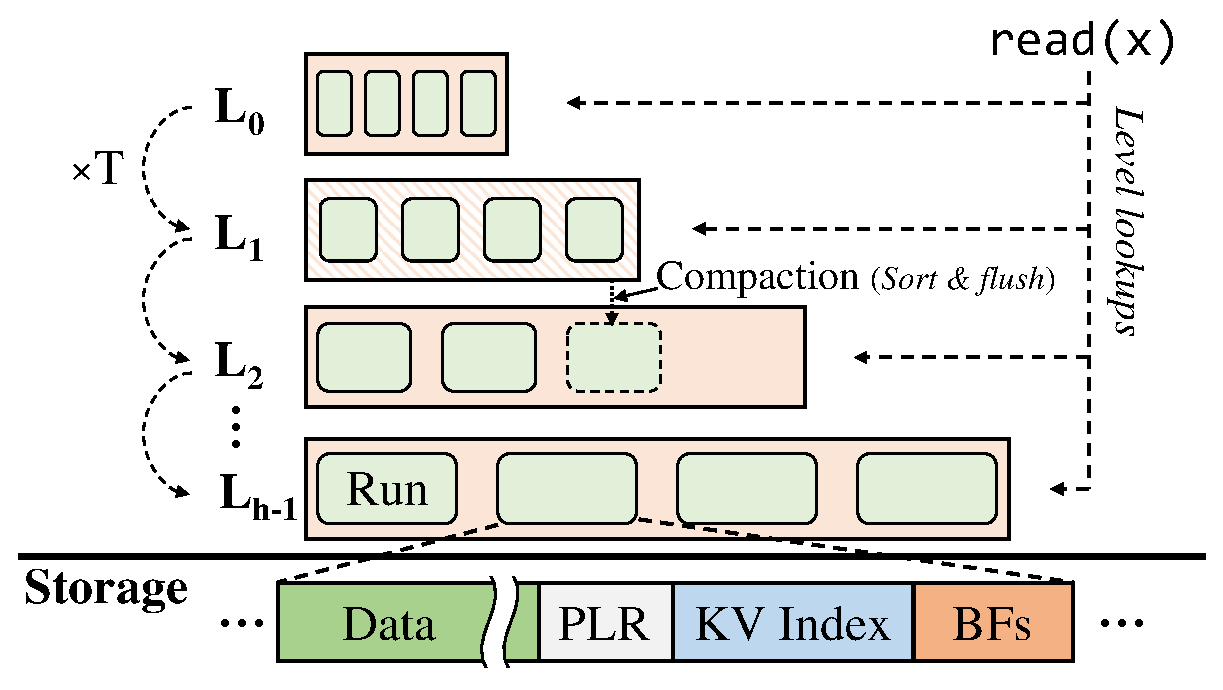
\includegraphics[height=3.3cm]{fig2.eps}
\includegraphics[height=2.4cm]{figs/figs-final/revised/plr-ctr.eps}
\vspace{-10pt}
\caption{FPR control in PLR}
\vspace{-10pt}
\label{fig:plr-control}
\end{figure}

\end{comment}





\subsection{Combining FP and PLR Indexing}
\label{sec:combine}

The FP- and PLR-based indexing behaves differently, thereby having different
memory requirements.  
The FP-based indexing requires 7.89-bit per
entry all the time. The PLR-based indexing requires 
51.2-bit per line segment, on average,
and thus its memory efficiency is decided by how many 
$<x_i,y_i>$ pairs are expressed by a line segment. In our setting, 
once each line segment 
can express more than 6.5 $<x_i,y_i>$ pairs, 
PLR outperforms FP, requiring less than 7.89-bit per
entry. Otherwise, using FP-based indexing is more beneficial. 

According to our analysis, the PLR-based indexing begins to outperform FP
when it is used for lower levels in the tree.
This is an expected result.  As a level gets larger in
size, many <$x_i$, $y_i$> pairs are densely sorted over a larger run and thus
can be efficiently expressed by a fewer equations.
We plot the number of bits per mapping entry while varying the run size (the
unit run size is 10GB and the storage capacity is 1TB) in
\FIG{fig:bf-plr-bit}(a).  
\FIG{fig:bf-plr-bit}(b) also shows the number of entries expressed
by a line segment.
%For small runs, the BF-based indexing is better, but as the
%run size grows, the PLR achieves better memory
%efficiency.  

\begin{comment}
%maintains a bitmap
%per entry, the PLR may require less memory as it can express many entries
using a few equations.  However, the memory usage of the PLR highly depends on
which level it is assigned.  \FIG{fig:overall:merged-maps} shows the number of
mapping entries expressed by a single linear equation at $L_i$ (from $L_1$ to
$L_{h-1}$).  As many entries are expressed by a linear equation, the PLR
achieves higher memory efficiency. For the middle levels
($L_1$$\sim$$L_{k-1}$), the PLR coalesces 2$\sim$7.89 entries per
equation.  Let us assume that each component of the linear equation requires
8B, 32B in total.
For the levels $L_1$$\sim$$L_{k-1}$, the PLR requires more memory,
16B$\sim$4.05B per mapping entry, than the typical index table where each entry
is 4B.  However, for the lower levels ($L_k$$\sim$$L_{h-1}$), the PLR
coalesces 8.47$\sim$13.52 entries, becoming more efficient than the
typical index table.  This is an expected result.  As a level gets larger in
size, many <$x_i$, $y_i$> pairs are densely sorted over a larger run and thus
can be efficiently expressed by a fewer equations.  Generally speaking, placing
the PLR in lower levels is beneficial; on the other hand, the BF is preferred
to be placed in middle levels.
\end{comment}

%As will be discussed in \SEC{sec:design}, depending on the implementation of the BF-
%and PLR-based indexing, their memory requirements differ greatly. Moreover, 
%\todo{
Given a specific tree, we can achieve the best memory efficiency
by assigning one (either FP or PLR) 
that requires less memory to each run.
However, depending on how the LSM-tree is organized, the size of levels and runs changes,
which affects the assignment of the approximation algorithm.  
We discuss this issue in detail in \SEC{sec:design:tree},
while exploring various organizations of the LSM-tree.


\begin{comment}
The BF- and PLR-based indexing behaves differently, thereby having different
memory requirements.  Compared to the BF-based indexing that maintains a bitmap
per entry, the PLR may require less memory as it can express many entries
using a few equations.  However, the memory usage of the PLR highly depends on
which level it is assigned.  \FIG{fig:overall:merged-maps} shows the number of
mapping entries expressed by a single linear equation at $L_i$ (from $L_1$ to
$L_{h-1}$).  As many entries are expressed by a linear equation, the PLR
achieves higher memory efficiency. For the middle levels
($L_1$$\sim$$L_{k-1}$), the PLR coalesces 2$\sim$7.89 entries per
equation.  Let us assume that each component of the linear equation requires
8B, 32B in total.
For the levels $L_1$$\sim$$L_{k-1}$, the PLR requires more memory,
16B$\sim$4.05B per mapping entry, than the typical index table where each entry
is 4B.  However, for the lower levels ($L_k$$\sim$$L_{h-1}$), the PLR
coalesces 8.47$\sim$13.52 entries, becoming more efficient than the
typical index table.  This is an expected result.  As a level gets larger in
size, many <$x_i$, $y_i$> pairs are densely sorted over a larger run and thus
can be efficiently expressed by a fewer equations.  Generally speaking, placing
the PLR in lower levels is beneficial; on the other hand, the BF is preferred
to be placed in middle levels.

As will be discussed in \SEC{sec:design}, depending on the implementation of the BF-
and PLR-based indexing, their memory requirements differ greatly. Moreover, 
depending on how the LSM-tree is organized, the size of levels and runs changes,
which affects the assignment of the approximation algorithm.  
We discuss this issue in detail in \SEC{sec:design:tree},
while exploring various organizations of the LSM-tree.
\end{comment}


\begin{comment}
In the middle levels ($L_1$$\sim$$L_{k-1}$), PLR-indexing does not coalesce
mapping entries enough to overcome its memory requirement.  As the runs in the
middle levels have fewer mapping entries, they have sparsely sorted mapping
pairs that make the memory efficiency of PLR-indexing worse.  Thus, we place
BF-indexing in the middle levels since BF-indexing always has the same memory
usage under the same FPR.  As the better memory-efficient approximate
algorithms are different by level, we assign the proper indexing algorithms to
level before running.  But, the memory-efficient setup for approximate
techniques may harm I/O performance and the total memory requirements of
\OURS{}.  To figure out the appropriate setup, we explore various \OURS{}
parameters by considering \ours{}'s I/O performance and memory usage in
\SEC{sec:design:tree}.
\end{comment}


\begin{comment}
\begin{figure}[t]
\centering
\includegraphics[width=0.4\textwidth]{figs/figs-final/revised/level-PLR.eps}
\vspace{-10pt}
%\caption{\fixme{The number of mapping entries in a function of PLR}}
\caption{The number of mapping entries per PLR equation}
\vspace{-10pt}
\label{fig:overall:merged-maps}
\end{figure}
\end{comment}


\begin{comment}
\todo{
The BF- and PLR-based indexing behaves differently, thereby having different
characteristics, in terms of indexing building cost, memory
efficiency, and lookup latency.  Compared to the BF-based indexing that 
builds tables by invoking a hash function supported by CPU instructions,
rebuilding PLR models takes longer as it requires many arithmetic operations.
Conversely, the PLR models exhibit high compression ratio as the size of a run gets larger.
This is because mapping pairs are likely to be densely sorted in the run,
which enables us to express many mapping pairs using fewer linear functions.
On the other hand, the BF-based indexing suffers from long lookup latency over a large run
because it perform search operations (\ie~binary search and scanning) over a larger run.
Those observations lead us to use the BF-based indexing on middle level where
runs are relatively small in size and compaction (\ie~model rebuilding) is
frequently triggered.  On the other hand, the PLR-based indexing is suitable
for lower levels that have larger runs and where compaction occasionally
happens.}  \todo{In \SEC{todo}, we explain the best cutting of the levels for BF
and PLR; 최적의 장소를 찾는 것은 시뮬레이션으로 할 수 있기 때문에 쉬움.
대신 최적의 메모리와 성능을 찾을 수 있도록 tree를 organization하는것은 생각이 필요함... 
이 부분이 강조 되어야할 듯..}
\begin{figure}[t]
\centering
\includegraphics[width=0.345\textwidth]{figs/figs-final/revised/level-PLR.eps}
\caption{\fixme{The number of mapping entries in a function of PLR}}
\label{fig:overall:merged-maps}
\end{figure}

\JS{윗 문단 대신 적으면 좋을듯. 
Because the each function in PLR-indexing manages many mapping entries,
PLR-based indexing has usually less memory requirement than BF-indexing.
However, the memory usage of PLR-indexing highly depends on where runs are
placed.  \FIG{fig:overall:merged-maps} shows the number of coalesced mapping
entries in each PLR function on different levels (\ie~$L_1$$\sim$$L_{h-1}$).
In the middle levels ($L_1$$\sim$$L_{k-1}$), PLR-indexing does not coalesce
mapping entries enough to overcome its memory requirement.  As the runs in the
middle levels have fewer mapping entries, they have sparsely sorted mapping
pairs that make the memory efficiency of PLR-indexing worse.  Thus, we place
BF-indexing in the middle levels since BF-indexing always has the same memory
usage under the same FPR.  As the better memory-efficient approximate
algorithms are different by level, we assign the proper indexing algorithms to
level before running.  But, the memory-efficient setup for approximate
techniques may harm I/O performance and the total memory requirements of
\OURS{}.  To figure out the appropriate setup, we explore various \OURS{}
parameters by considering \ours{}'s I/O performance and memory usage in
\SEC{sec:design:tree}.
}
\end{comment}

%\subsection{Impact of Tree organization on Memory and WAF}
%\subsection{Approximate Indexing using BF and PLR}




%\subsection{Combining BF and PLR in LSM-tree}
\subsection{Tree Organization and Its Impacts}
%Combining BF and PLR in LSM-tree}
\label{sec:design:tree}
\begin{figure}[t]
\centering
     \begin{subfigure}[b]{0.21\textwidth}
         \centering
         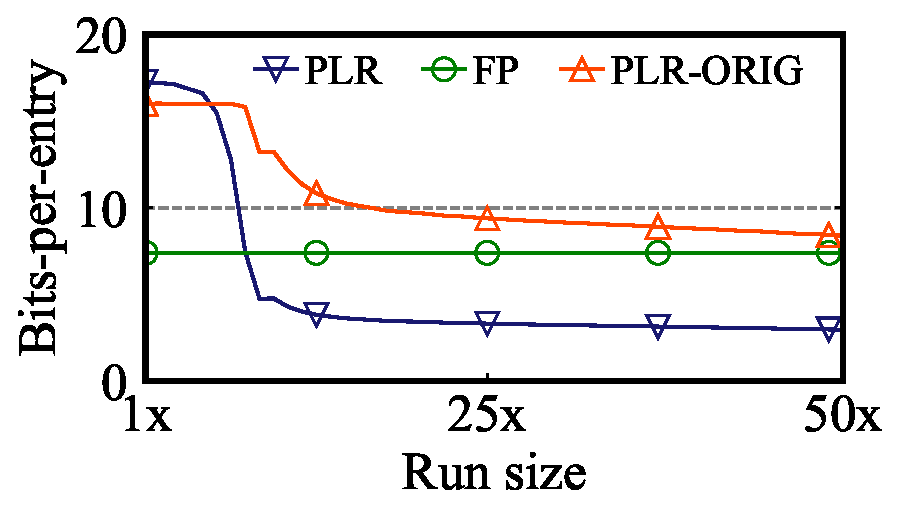
\includegraphics[width=\textwidth]{figs/OSDI/exp_data/bit-per-entry/OURS-BF-PLR.eps}
         \vspace{-10pt}
         \caption{\# of bits per entry}
     \end{subfigure}
     \hfill
     \begin{subfigure}[b]{0.21\textwidth}
         \centering
         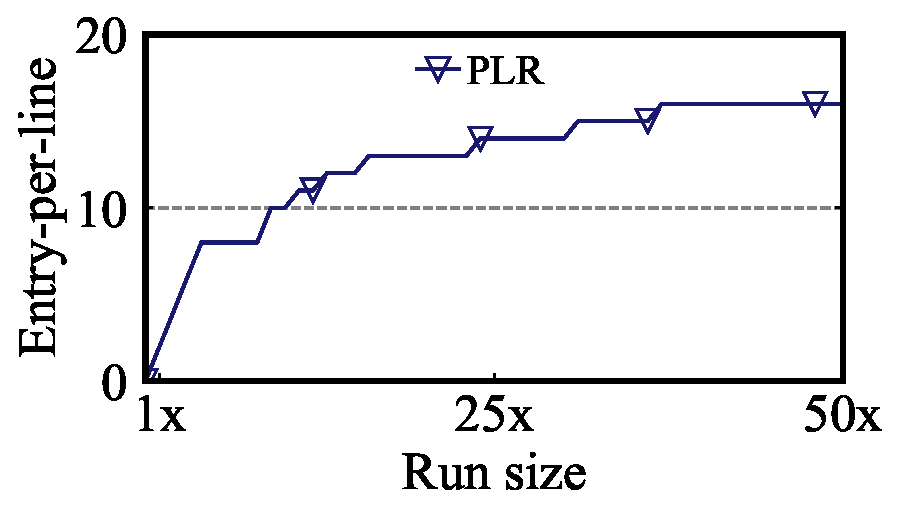
\includegraphics[width=\textwidth]{figs/OSDI/exp_data/line-per-entry/PLR-Range.eps}
         \vspace{-10pt}
         \caption{\# of entries per line}
     \end{subfigure}
       \vspace{-10pt}
     \caption{Memory usage of FP and FPR depending a run size}
%     \caption{\fixme{\# of bits per entry and \# of entries per line in PLR}}

     \label{fig:bf-plr-bit}
\end{figure}




\begin{comment}
\begin{figure*}[t]
     \centering
     \begin{subfigure}[b]{0.175\textwidth}
         \centering
         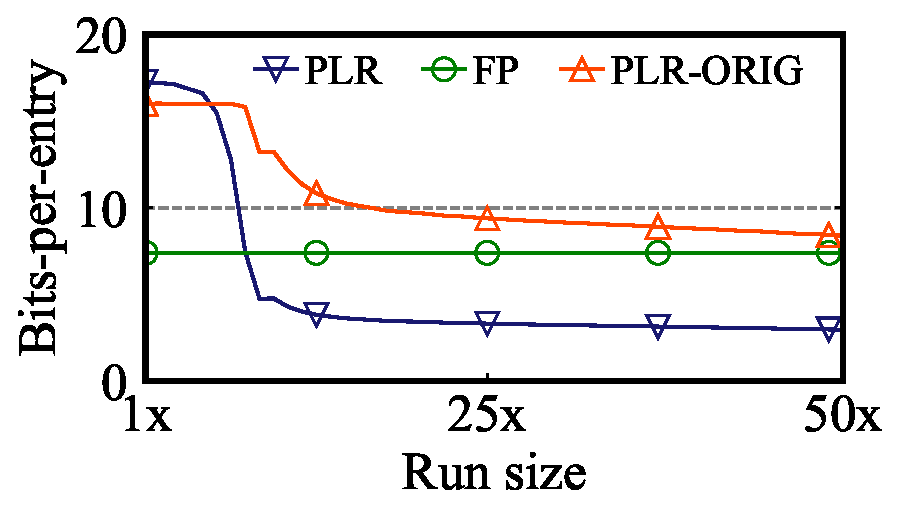
\includegraphics[width=\textwidth]{figs/OSDI/exp_data/bit-per-entry/OURS-BF-PLR.eps}
         \caption{\# of bits per entry}
     \end{subfigure}
     \hfill
     \begin{subfigure}[b]{0.175\textwidth}
         \centering
         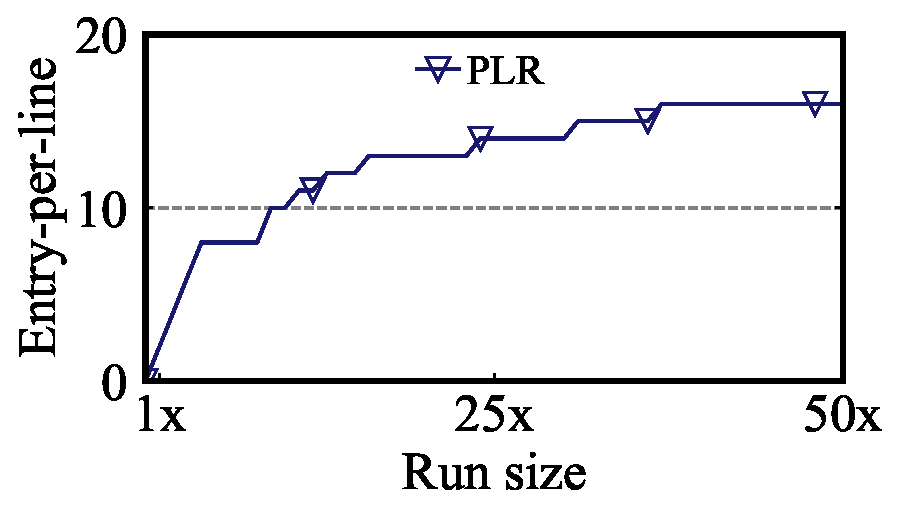
\includegraphics[width=\textwidth]{figs/OSDI/exp_data/line-per-entry/PLR-Range.eps}
         \caption{\# of entry per line}
     \end{subfigure}
     \hfill
     \begin{subfigure}[b]{0.28\textwidth}
         \centering
         \includegraphics[width=\textwidth]{figs/Figure_lsm_design/lsm_design/3d_memory/3d_memory2.eps}
         \caption{Memory usage depending $T$ and $|L_0|$}
     \end{subfigure}
     \hfill
     \begin{subfigure}[b]{0.28\textwidth}
         \centering
         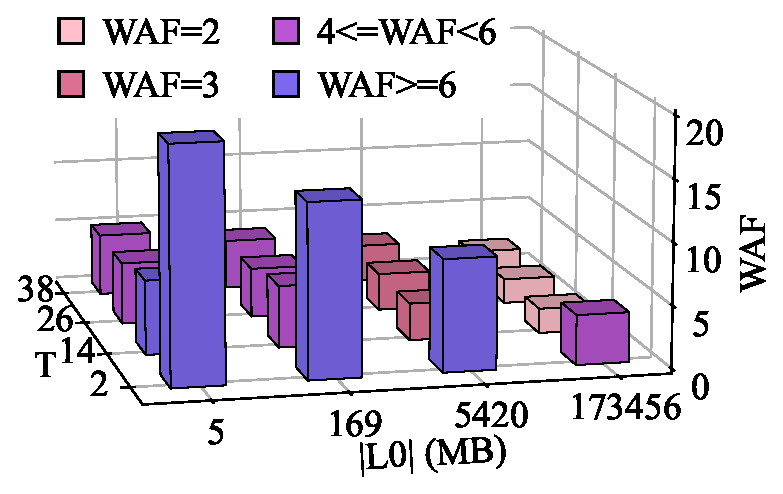
\includegraphics[width=\textwidth]{figs/Figure_lsm_design/lsm_design/3d_waf/3d_waf_2.eps}
         \caption{WAF depending $T$ and $|L_0|$}
     \end{subfigure}

	 \caption{Memory and performance analysis of \ours{} depending on tree organization}
\label{fig:tree-org}
\end{figure*}
\end{comment}

\begin{comment}
\begin{figure*}[t]
     \centering
     \begin{subfigure}[b]{0.175\textwidth}
         \centering
         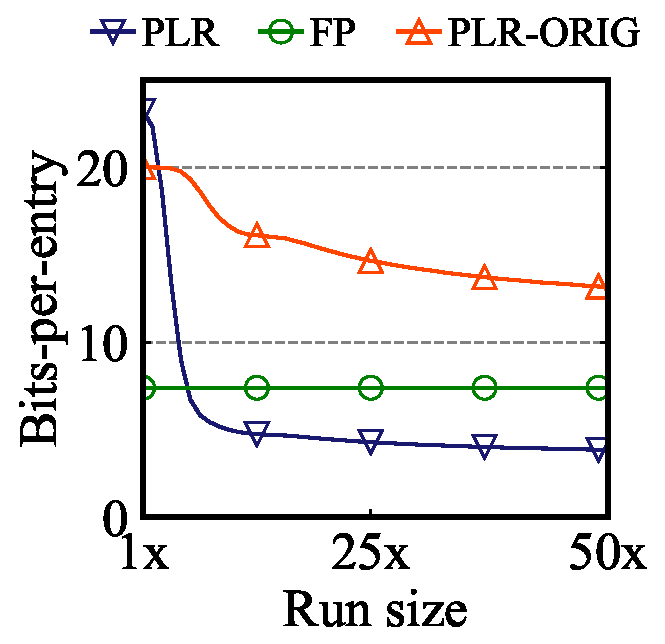
\includegraphics[width=\textwidth]{figs/Figure_lsm_design/lsm_design/BF-PLR/OURS-BF-PLR.eps}
         \caption{\# of bits per entry}
         \label{fig:tree-org}
     \end{subfigure}
     \hfill
     \begin{subfigure}[b]{0.28\textwidth}
         \centering
         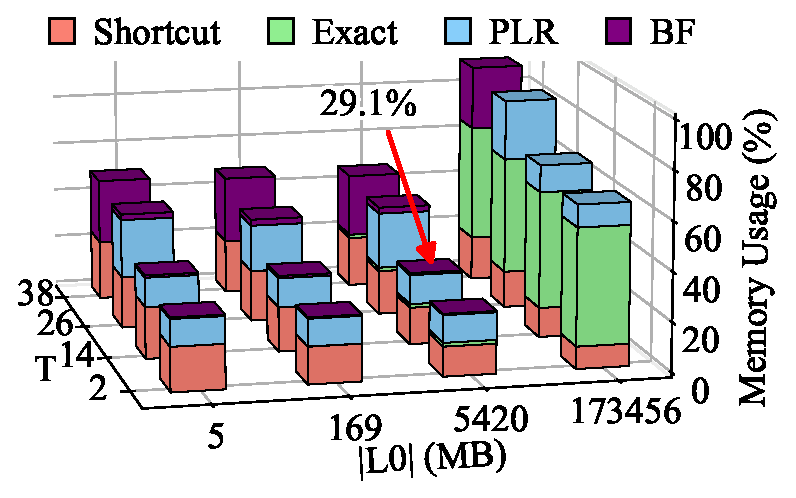
\includegraphics[width=\textwidth]{figs/Figure_lsm_design/lsm_design/3d_memory/3d_memory.eps}
         \caption{Memory usage depending $T$ and $|L_0|$}
         \label{fig:tree-org}
     \end{subfigure}
     \hfill
     \begin{subfigure}[b]{0.28\textwidth}
         \centering
         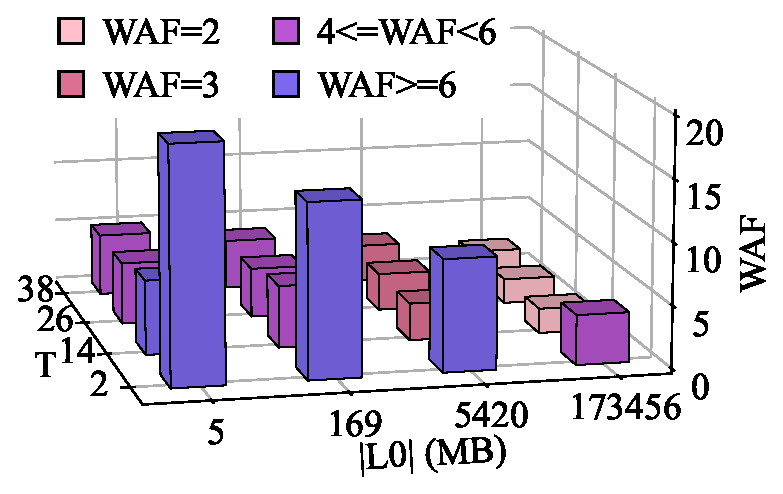
\includegraphics[width=\textwidth]{figs/Figure_lsm_design/lsm_design/3d_waf/3d_waf_2.eps}
         \caption{WAF depending $T$ and $|L_0|$}
         \label{fig:tree-org}
     \end{subfigure}
     \hfill
     \begin{subfigure}[b]{0.202\textwidth}
         \centering
         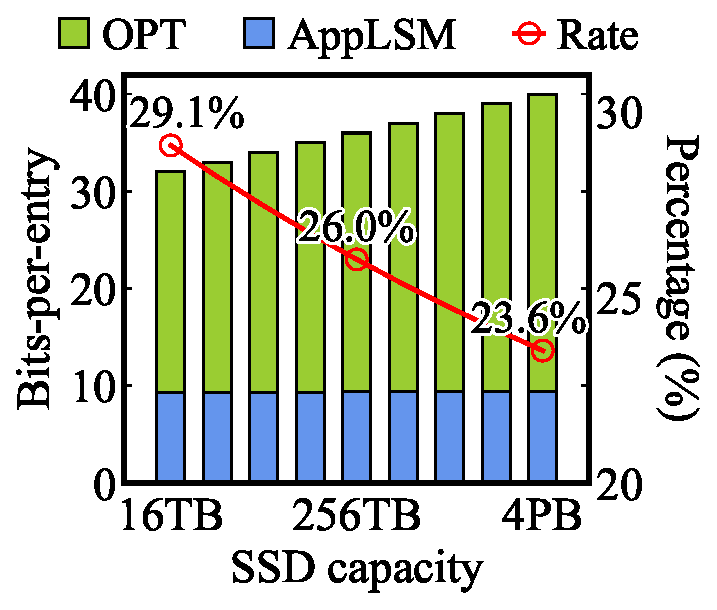
\includegraphics[width=\textwidth]{figs/Figure_lsm_design/lsm_design/scale/twinx-scale.eps}
         \caption{Scalability w/ SSD size}
         \label{fig:tree-org}
     \end{subfigure}
	 \vspace{-10pt}
	 \caption{Memory and performance analysis of \ours{} depending on tree organization, \FIXME{BF-->FP, add PLR original to (a)}}
	 \vspace{-10pt}
\label{fig:tree-org}
\end{figure*}
\end{comment}


%In this section, we explore the optimal organization of the LSM-tree to maximize
%the memory efficiency of both the BF- and PLR-based indexing algorithms when
%they are used together.  
In this section, we explore the organization of an LSM-tree and analyze
its impact on the memory usage when FP and PLR are used together.  
The tree organization also has a high impact on
write performance since WAF varies depending on a tree height $h$
as we mentioned before (see~\SEC{sec:back:lsm-tree}).  
We discuss how to derive a balanced tree hierarchy that
satisfies both memory efficiency and high write throughput.

\begin{comment}
The two approximate algorithms 
show different performance and memory usages depending on which level they are assigned. 
This section
explores how the optimal tree organization can be derived in a manner
that minimizes the memory requirement. We also consider the
impact of the tree organization on the write amplification factor (WAF)
($=\frac{\text{data written to flash}}{\text{data written by host}}$).
\end{comment}


%\st{\textbf{Impact of tree organization on memory.}}
%\JS{\textbf{Impact of run size on approximate indexing techniques.}}
\begin{comment}
As discussed in \SEC{sec:design:bf-plr-basic}, 
the PLR-based indexing provides high memory efficiency when a run size is large.  
%As the run gets larger, mapping pairs are likely to be more densely sorted within the run,
%which enables us to express many entries using fewer equations. 
Conversely, regardless of the run size, the BF-based indexing requires the same number of bits
per entry. This is because a BF entry size is decided by a target
FPR and the number of BFs to be tested (see \EQ{eq:fpr-relax}). Those parameters are decided at the design time
(\eg~$FPR_{T}$=0.1 and $n$=28 in \SEC{sec:opt:memory}) and 
are the same for all the runs. 
We plot the number of bits per mapping entry while varying the run size (the
unit run size is 10GB and the storage capacity is 1TB) in
\FIG{fig:tree-org}(a).  For small runs, the BF-based indexing is better, but as the
run size grows, the PLR achieves better memory
efficiency.  
%\todo{
Given a specific tree, we can achieve the best memory efficiency
by assigning one (either BF- or PLR-based indexing) 
that requires less memory to each level.
%make it decide which
%algorithms should be assigned to which layer; we just need to choose the most memory
%efficient one. (이러한 분위기로...)}
%It also shows how better memory-optimized it is compared to the
%original PLR (denoted as \texttt{PLR(ORIG)}).  
\end{comment}

Our results in \SEC{sec:combine} suggests that
it is desirable to increase the average run size if possible.
It may increase the likelihood that more runs are managed 
by memory-efficient PLR models.
%further reducing the memory usage of the tree.
Let $R_{avg}$ be the average run size in the tree.
$R_{avg}$ is obtained by dividing the storage capacity ($CAP$)
by the total number $r_{tot}$ of runs in the tree. In \ours{}, the
top level $L_0$ has a single run (see~\SEC{design:overall}). From $L_1$ to $L_{h-1}$, the
number $r$ of runs per level is the same. If the tree height is
$h$, $r_{tot}$ is $(h-1) \cdot r + 1$. 
$R_{avg}$ is thus defined as follows:
\begin{equation}
\small
\begin{split}
	R_{avg}=\frac{CAP}{(h-1) \cdot r + 1}.
\end{split}
\label{eq:r_avg_original}
\end{equation}

By reducing $h$ and $r$, we make $R_{avg}$ larger. 
Changing the run size is not easier than it appear to be.
This is because $h$ and $r$ are also decided by two tree parameters,
(\textit{i}) the size factor $T$ and (\textit{ii}) the size of $L_{0}$, 
which affect the memory usages of other components, 
the RB-tree for $L_0$ and the shortcut table.
%Thus, we should choose the proper $T$ and size of $L_0$ considering their impacts.
%on performance and memory.

%I/O performance and 
%total memory usage of \ours{}.
%To figure out the relationship among $R_{avg}$, I/O performance and the total memory requirement, 
%we reorganize \EQ{eq:r_avg_original} by using $T$ and size of $L_0$.


Let us express $h$ using the size factor $T$ and the size of $L_0$.
%\st{To obtain $h$, let}\JS{First, we define $h$ by the two variables. Let} 
Let $|L_i|$ be the size of $L_i$ in the tree.
$|L_i|$ increases by a factor of $T$ from the
top-level $L_0$, that is, $|L_{i}| = |L_0| \cdot T^{i}$ ($0<i<h$), where $i$ is
the level number.  $h$ 
%the level number and $h$ is the tree height.  $h$ 
is thus defined as follows (detailed derivation steps are given in~\cite{monkey}):
\begin{equation}
\small
\begin{split}
	h &= \ceil*{log_{T}\left(\frac{CAP}{|L_0|} \right)}.
\end{split}
\label{eq:n_level}
\end{equation}
\begin{comment}
\st{where $C$ is the SSD capacity.}
%If $C$ = 1 TB, $|L_0|$ = 256 MB, and
%$T$ = 4, $h = 6$. 
\st{Since $C$ is fixed in our setup, $|L_0|$ and $T$ decide
the tree height $h$. 
As $L_0$ and $T$ get larger, the tree becomes fatter and $h$ becomes smaller, 
and vice versa.}
%As will be discussed later, the tree height has a high impact on WAF.
\end{comment}

%$T$ also represents the number $N_{run}$ of runs per level in \ours{}.
%\st{$T$ decides the number $N_{run}$ of runs per level.}
In LSM-trees, $r = T$.  The proof is straightforward.  For compaction
of $L_i$ and $L_{i+1}$, \ours{} reads all the runs $R_i$ at $L_i$, merges and
sorts data, and write them to $L_{i+1}$, creating a new run $R_{i+1}$.
The size $|R_{i+1}|$ of $R_{i+1}$ is thus equal to $|L_i|$.  For $|L_{i+1}|$ to
be $T$ times larger than $|L_{i}|$, $L_{i+1}$ should have $T$ runs.  
\begin{comment}
\begin{equation}
\small
\begin{split}
	r &= T.
\end{split}
\label{eq:n_run}
\end{equation}
\end{comment}

\begin{figure}[t]
     \centering
     \begin{subfigure}[b]{0.23\textwidth}
         \centering
         \includegraphics[width=\textwidth]{figs/Figure_lsm_design/lsm_design/3d_memory/3d_memory2.eps}
         \caption{Memory usage}
     \end{subfigure}
     \hfill
     \begin{subfigure}[b]{0.23\textwidth}
         \centering
         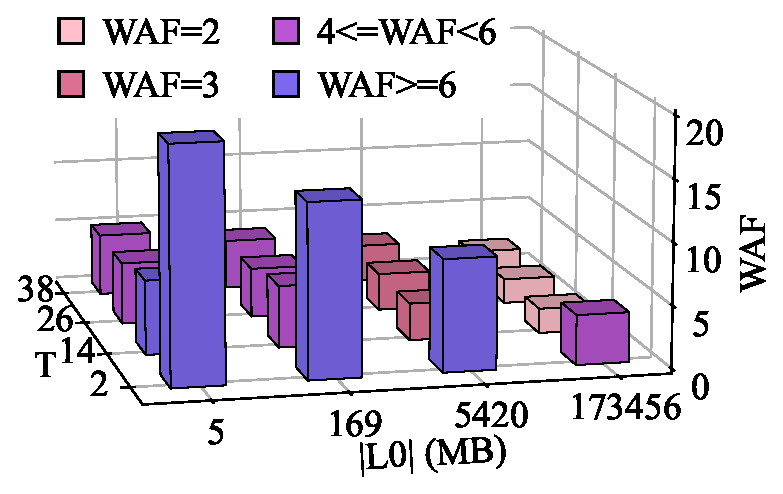
\includegraphics[width=\textwidth]{figs/Figure_lsm_design/lsm_design/3d_waf/3d_waf_2.eps}
         \caption{WAF}
     \end{subfigure}  
     \vspace{-5pt}

	 \caption{Memory usage and WAF depending $T$ and $|L_0|$}
  \vspace{-5pt}
\label{fig:tree-org}
\end{figure}

%Using Eqs.~(\ref{eq:n_level}) and~(\ref{eq:n_run}), 
Using Eq.~(\ref{eq:n_level}), \EQ{eq:r_avg_original} can be 
rewritten as follows:
\begin{equation}
\small
\begin{split}
	R_{avg} &= \frac{CAP}{(h-1) \cdot r + 1} = \frac{CAP}{(\ceil*{log_{T}\left(\frac{CAP}{|L_0|} \right)}-1)\cdot T+1}.
\end{split}
\label{eq:r_avg}
\end{equation}

\EQ{eq:r_avg} tells us that $R_{avg}$ can be increased 
by reducing $T$ and increasing $|L_0|$, and vice versa.

We measure the memory usage
and WAF of \ours{} while varying $T$ and $|L_0|$,
\FIG{fig:tree-org}(a) illustrates the memory usage (\%) of
\ourtree{}, relative to the optimal FTL.
We break down the graph to highlight
the memory usage of four key components:
FPs, PLR models, the RB-tree for $L_0$, 
and the shortcut table.  
For each level, either the FP- or
PLR-based indexing can be used.  We choose one that requires less memory.  

We
make two key observations.  First, the memory requirement 
is mainly decided by $T$.  The smaller $T$, the larger the memory
savings as a run gets larger in size.
As $T$ increases, the memory efficiency of PLR rapidly drops, and
at $T=38$, PLR is no longer useful. % owing to the small run size.
Instead, using FP is more beneficial.  Additionally, 
the shortcut table size is proportional to $r$, 
it gets smaller as $T$ reduces.
Second, the size of $L_0$ has a negligible impact on memory
usage. By increasing $|L_0|$, we can make 
$R_{avg}$ larger.
However, since $R_{avg}$ increases logarithmically as $|L_0|$,
its impact is not huge.
However, when $L_0$ increases too large, 
the RB-tree consumes lots of DRAM.

\FIG{fig:tree-org}(a) displays the WAFs of the trees for the same combinations
of $T$ and $L_0$ in \FIG{fig:tree-org}(b).  
%In LSM-trees, whenever compaction is triggered, valid data stored
%in $L_i$ are copied to a new run in the
%next level, $L_{i+1}$. 
%As the tree becomes taller, the compaction cost gets higher
%because compaction is more frequently invoked~\cite{monkey}.
%As a result, the WAF of \ourtree{} is directly proportional
%to $h$ in \EQ{eq:n_level}. \FIG{fig:tree-org}(d)  supports this fact well;
According to \EQ{eq:n_level},
as $T$ and/or $L_0$ get smaller, the tree becomes taller,
which results in an increase of $h$.
As mentioned in \SEC{sec:back:lsm-tree}, with higher $h$, 
the overall WAF of the tree increases.

From Figs.~\ref{fig:tree-org}(a) and (b), we notice that there exists a
trade-off between the memory and WAFs.  To minimize the memory requirement, it
is preferred to set $T$ very small with a balanced $|L_0|$.  
But, for write throughput, 
setting $T$ and $|L_0|$ very large is a good choice.
However, in most cases, a balanced tree would be preferred.  
When $T=14$ and $|L_0|$ = 5.4GB, \ourtree{} reduces the memory
space to 29.1\% compared to the optimal FTL 
with the reasonable WAF of 3.  With the balanced option,
\ours{} is organized with three levels: 
$L_0$ with RB-tree, $L_1$ with FP indices, and $L_2$ with PLR models.

\begin{comment}
\todo{(실험 결과에 넣는것이 좋을 듯)}

\textbf{Scalability issue:}
As SSD capacity increases, each entry of the typical index table requires more
bits because it has to cover larger physical space.  For a 16TB SSD, a 32-bit
table entry is enough, but it increases to 35-bit when an SSD size
increases to 128TB.  The number of entries per table increases as well.
Compared to typical FTLs, \ours{} provides better scalable in terms of memory.
By increasing a run size, we can keep using the balanced setup,
regardless of SSD capacity.  The tree parameters, $T$, $h$, and $r$, remain the
same.  To cover larger physical space, the number of FP indices and PLR
equations in the tree increases, but the number of bits per FP-entry and
PLR-equation does not.  As pointed out before, the FP size is decided by
\JS{$\mathcal{E}_{FP}$ and $k$}.  \fixme{$x_0^i$ and $y_0^i$ of $S_i$} increase, but since they are
delta-encoded over sorted fragments, we can express them using the same
number of bits (\ie~11-bit and 9-bit).  
%\sout{Only the
%exceptions are the exact indices for $L_0$, guards of BF-indexing that point
%to exact locations $y_i$ of physical sectors.}
Only the exceptions are the \JS{RB-tree} for $L_0$, \JS{the first entries of FP groups 
and delta-encoded PLR groups}.
However, since the \JS{RB-tree} and the FP-based indexing occupy
only about 5\% of the total memory usage (see \FIG{fig:tree-org}(c)) and
the pivots occupy 0.06\%, their
impacts on the total memory are negligible.  \FIG{fig:scalability} compares the
number of bit per entry of the optimal FTL and \ours{}.  The optimal FTL needs
more bits per entry as the SSD capacity gets larger, but \ours{} has almost the
same bits per entry, exhibiting better scalability.
\end{comment}

\subsection{Crash Consistency}
Approximate indices that reside in
DRAM are immutable and thus all clean. The loss of them
on a crash does not make the system inconsistent. The
memtable, the shortcut table, and the RB-tree, however,
keep dirty indices and data in memory, 
so their loss may lead to the inconsistent system.
The loss of buffered data in the memtable is inevitable 
(unless it is backed by capacitors), but
it does not hurt consistency like other log-structured systems.  
The RB-tree is rebuilt by scanning small $L_0$ 
as LBAs of data are recorded in OOBs. 
However, the reconstruction of the shortcut table is challenging
as it takes so long to scan the entire tree.  
To address this, when the memtable is flushed out to $L_0$ 
or runs are compacted with the next level,
\ours{} writes associated shortcut-table entries to run's metadata.
During recovery, 
we can quickly rebuild the shortcut table 
by reading run's metadata.



\begin{comment}
\JS{
This balanced tree setup can be adopted to any storage capacities by scaling $|L_{0}|$.
If \ours{} has the same values of $\frac{C}{|L_0|}$ and $T$ in different storage capacities, 
it has the similar I/O performance and memory requirement (see Eq.~(\ref{eq:n_level}) and (\ref{eq:r_avg})).
Some data structures (\ie~guard of BF-indexing and exact indexing for $L_0$) 
may need more bits than 32-bit as the physical storage gets larger.
However, they occupies only about 5\% of the total memory usage in balanced tree setup as shown in \FIG{fig:tree-org}(b).
Thus, the effects of these data structures on the total memory are negligible.
\FIG{fig:tree-org}(d) shows the impact of storage capacities on the \ours{}
memory usage with balanced tree parameters and 0.1 FPR.
The optimal FTL needs more bits per entry as the storage capacity gets larger, but 
\ours{} has almost the same bit per entry. 
As a result, the memory usage ratio between \ours{} and the optimal FTL goes down.
}
%For read-only applications where write
%throughput is not as important, 
%the tree with smaller $T$ and $L_0$ might be better.  Conversely, for write-heavy applications, we have to trade memory for
%lower WAF. 
\end{comment}

\begin{comment}
Once tree organization is decided, we can fine-tune RAF
and memory by changing FPR. By increasing FPR, we further reduce the memory
requirement, sacrificing read latency, and vice versa.  \FIG{fig:tree-org}(d)
is the memory usage by FPR. 
\end{comment}

\begin{comment}
\begin{figure*}[!t]
    \begin{minipage}[c]{0.28\textwidth}
            \centering
            \vspace{2pt}
            \includegraphics[width=\textwidth]{exp/miss_ratio/final-miss-ratio.eps}
            \vspace{-7pt}
   	        \caption{\FIXME{Miss ratio}} 
   	        \vspace{-10pt}
            \label{fig:miss-ratio}
    \end{minipage}
	\begin{minipage}[c]{0.71\textwidth}
        \begin{subfigure}[b]{0.64\textwidth}
            \centering
            \includegraphics[width=\textwidth]{exp/filesystem/fs-latency.eps}
            \vspace{-10pt}
   	        \caption{\FIXME{Read latency}} 
            \label{fig:swap-latency}
        \end{subfigure}
        \begin{subfigure}[b]{0.345\textwidth}
            \centering
            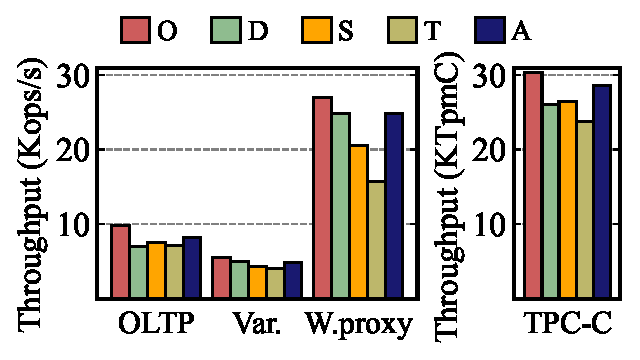
\includegraphics[width=\textwidth]{exp/filesystem/final-fs-throughput.eps}
            \vspace{0pt}
            \caption{Throughput} 
            \label{fig:swap-throughput}
        \end{subfigure}
        \vspace{-10pt}
	    \caption{Experimental results of Filebench and TPC-C}
	    \vspace{-10pt}
	    \label{fig:exp-fs}
	\end{minipage}
\end{figure*}
\end{comment}


\section{Experiments}
\label{sec:exp}
We show experimental results using realistic benchmarks,
%Since we already presented microscopic results in
%\SEC{sec:new-design}, we 
focusing on three performance aspects of \ours{}:
(\textit{i}) read latency, (\textit{ii}) I/O throughputs,
and (\textit{iii}) computation overheads.
%We focus on evaluating following three
%aspects of \ours{}: (\textit{i}) read latency, (\textit{ii}) I/O
%throughputs, and (\textit{iii}) impact of write optimization.

\begin{figure*}[t]
	\begin{minipage}[c]{0.71\textwidth}
        \begin{subfigure}[b]{0.64\textwidth}
            \centering
            \includegraphics[width=\textwidth]{exp/filesystem/fs-latency.eps}
            \vspace{-10pt}
   	        \caption{Read latency}
            \label{fig:swap-latency}
        \end{subfigure}
        \begin{subfigure}[b]{0.345\textwidth}
            \centering
            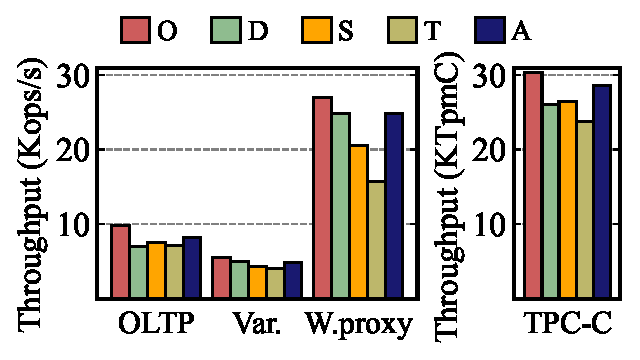
\includegraphics[width=\textwidth]{exp/filesystem/final-fs-throughput.eps}
            \vspace{-5pt}
            \caption{Throughput} 
            \label{fig:swap-throughput}
        \end{subfigure}
        \vspace{-7pt}
	    \caption{Experimental results of Filebench and TPC-C}
	    \vspace{-10pt}
	    \label{fig:exp-fs}
	\end{minipage}
    \begin{minipage}[c]{0.28\textwidth}
            \centering
            \vspace{0pt}
            \includegraphics[width=\textwidth]{exp/miss_ratio/real-final-miss-ratio.eps}
            \vspace{-2pt}
   	        \caption{Miss rate}
            \vspace{-5pt}
            \label{fig:miss-ratio}
    \end{minipage}
    \vspace{-5pt}
\end{figure*}
%\vspace{-5pt}
\subsection{Experimental Setup}
\label{sec:exp:setup}

All experiments are conducted on a machine with Intel's i9 CPU (12
cores running at 4.6 GHz) and 4GB DRAM. We use an FPGA-based PCIe
Open-channel SSD employing custom flash cards that has 512GB capacity
and offers
2.4 GB/s read and 860 MB/s write throughputs.
The page size is 16KB,
and the number of pages per block is 128.  
We implement various translation policies on the x86 host like
ones~\cite{dm-zoned, ocssd} for ZNS and OCSSD. 
For fast evaluation, the SSD capacity is set to
64GB.  The over-provisioning space is 15\%.

Including \ours{}, we implement four popular policies, the optimal FTL (denoted
by \texttt{OPT})~\cite{flash-based-ssd
}, DFTL~\cite{dftl}, 
SFTL~\cite{sftl}, and TPFTL~\cite{tpftl}.  
\OPT{} maintains all the exact mapping entries in DRAM.
%A mapping entry size is
%40-bit under the assumption that the SSD capacity is larger than 32-TB.
%For a indexing table, 80-MB DRAM -- 0.125\% of SSD's capacity --
%is required. 
\OPT{} is infeasible in that it consumes lots of DRAM, when the SSD size is
huge.
%Note that 32-TB SSD needs 33-bit for pointing all 4-KB sectors in SSD, but
%33-bit does not align in byte-address.
%To index mapping entries, all policies except for \SECTOR{}
%use 24\% (19.2-MB) of DRAM that \SECTOR{} requires.
\DFTL{} keeps only popular entries in DRAM that are managed by LRU. \SFTL{} and
\TPFTL{} are variants of \DFTL{}.  \SFTL{} behaves as explained in
\SEC{sec:back:table}.  \TPFTL{} improves a cache hit rate by employing
two-level LRUs: one for indexing chunks (ICs) and the other for mapping entries
within chunks.  It also delta-encodes consecutive mapping entries.  The main
difference between  \SFTL{} and \TPFTL{} is a caching granularity. In
contrast to \SFTL{} that caches mapping entries belonging to the same 4KB IC,
\TPFTL{} caches popular mapping entries (\ie~<$x_i$, $y_i$>) to efficiently
use DRAM space only for hot entries.
%(\ie~indexing chunk in \SFTL{} and mapping entry in \TPFTL{}).
\OURS{} uses the balanced tree setup with three levels, as explained in
\SEC{sec:design:tree}, but it scales down the L0 size from 5.4GB to 332MB
as we use a smaller SSD (1TB vs 64GB).  A target FPR is set to 0.1.  All the
FTLs use the 1MB write-buffer (the memtable in the case of \ours{}).
For indexing, \texttt{OPT} uses 64MB DRAM (0.1\% of 64GB) and
the other FTLs use 18.6MB (29.1\% of \texttt{OPT}'s memory).
%assuming that the underlying SSD capacity is 16TB.
%\todo{(DRAM for mapping table)}


%\fixme{
We evaluate the FTLs under three representative systems that use SSDs as file,
swap, and cache storage, respectively.
%We evaluate the FTL techniques in three representative systems that use SSDs as
%their storage (\ie~file system, swap, and cache system).  
For file-system benchmarks, we use two Filebench~\cite{filebench} and
TPC-C~\cite{TPC-C} that run on EXT4.  For file-system
aging, we run Geriatrix~\cite{geriatrix}, a fragmentation tool, over EXT4
before running benchmarks. 
%After the aging, the SSD utilization is 49\%.  
To
emulate a use case of SSDs as swap storage, we run YCSB~\cite{ycsb} over Redis,
a popular in-memory KV store~\cite{redis}.  Finally, to evaluate performance
when SSDs are used for a cache service, we run CacheLib~\cite{cachelib}.
%We also use YCSB~\cite{ycsb} and CacheLib~\cite{cachelib} as swap
%and cache system benchmarks, respectively.  Filebench and TPC-C are run on EXT4
%as the default file system.}
%To emulate aged file systems, we run Geriatrix~\cite{geriatrix}, a
%fragmentation tool, over EXT4 before running benchmarks. After the
%aging, the SSD utilization is 49\%.  

\subsection{Experimental results}
%\JS{We refer to the miss ratios and WAFs of FTL techniques
%on benchmarks to explain their performances. 
%All of the miss ratios and WAFs are illustrated in \FIG{fig:miss-ratio} 
%and Table~\ref{tab:waf}, respectively.}
%\JS{In all figures of experimental results, \texttt{OPT}, \texttt{DFTL}, \texttt{SFTL}, \texttt{TPFTL}, and \texttt{APX-FTL}
%are abbreviated as `\texttt{O}', `\texttt{D}', `\texttt{S}', `\texttt{T}', and `\texttt{A}'.}

\begin{comment}
\begin{figure}[t]
\centering
\includegraphics[width=0.93\linewidth]{exp/miss_ratio/new-miss-ratio.eps}
\vspace{-10pt}
\caption{\FIXME{Miss ratio}}
\vspace{-10pt}
\label{fig:miss-ratio}
\end{figure}
\end{comment}



\subsubsection{Results from File-system Benchmarks}
\label{sec:exp:fs}
%To evaluate \ours{} when it is used for file systems, we performs experiments
%using Filebench and TPC-C database benchmark.  
We choose three workloads from Filebench: \texttt{OLTP}, \texttt{Varmail}, and
\texttt{Webproxy}. The Filebench workloads have two phases, load and run.  In
the load phase, all workloads create files so that 77\% of the SSD is filled
with data. During the run phase, \texttt{Varmail} and \texttt{Webproxy} issue
8M and 4M operations over the created files, \texttt{OLTP} runs for 480
seconds.  In the case of TPC-C, we use PostgreSQL~\cite{postgresql} as RDBMS.
We create 220 warehouses before running TPC-C.  After creating the warehouses,
we run TPC-C for 10 minutes.

\begin{figure*}[t]
    %\vspace{0pt}
	\begin{minipage}[c]{0.622\textwidth}
        \begin{subfigure}[b]{0.45\textwidth}
            \centering
            \includegraphics[width=\textwidth]{exp/swap/swap-latency.eps}
            \vspace{-13pt}
   	        \caption{Read latency}
            \label{fig:swap-latency}
        \end{subfigure}
        \begin{subfigure}[b]{0.51\textwidth}
            \centering
            \vspace{0pt}
            \includegraphics[width=\textwidth]{exp/swap/new_SWAP_throughput.eps}
            \vspace{-1pt}
            \caption{Throughput} 
            \label{fig:swap-throughput}
        \end{subfigure}
        \vspace{-10pt}
	    \caption{Experimental results of YCSB benchmark}
	    \label{fig:exp-swap}
	    \vspace{-15pt}
	\end{minipage}
	\begin{minipage}[c]{0.368\textwidth}
        \begin{subfigure}[b]{0.52\textwidth}
            \centering
            \vspace{8pt}
            \includegraphics[width=\textwidth]{exp/cache/cache-latency.eps}
   	        \caption{Read latency}
            \label{fig:cache-latency}
        \end{subfigure}
        \hspace{5pt}
        \begin{subfigure}[b]{0.32\textwidth}
            \centering
            \includegraphics[width=\textwidth]{exp/cache/new_cache_th.eps}
            \vspace{-9pt}
            \caption{Throughput} 
            \label{fig:cache-throughput}
        \end{subfigure}
        \vspace{-10pt}
	    \caption{Experimental results of cache system}
	    \vspace{-15pt}
        \label{fig:expcache}
    \end{minipage}

\end{figure*}

\begin{comment}
\begin{figure}[t]
    \centering
    \includegraphics[width=0.28\textwidth]{figs/Figure_lsm_design/lsm_design/scale/plr-scale.eps}
    \caption{Scalability w/ SSD size}
    \label{fig:scalability}
\end{figure}
\end{comment}

\begin{comment}
\begin{figure}[t]
    %\vspace{0pt}
    \begin{subfigure}[b]{0.475\textwidth}
        \centering
        \includegraphics[width=\textwidth]{exp/filesystem/fs-latency.eps}
        \caption{Read latency}
        \label{fig:fs-latency}
        \vspace{5pt}
    \end{subfigure}
    \begin{subfigure}[b]{0.38\textwidth}
        \centering
        \includegraphics[width=\textwidth]{exp/filesystem/FS_throughput.eps}
        \caption{Throughput} 
        \label{fig:fs-throughput}
    \end{subfigure}
    \vspace{-10pt}
    \caption{Experimental results of Filebench and TPC-C}
    \label{fig:exp-fs}
    \vspace{-10pt}
\end{figure}
\end{comment}

\FIG{fig:exp-fs}(a) shows the average read latency, 
along with 50$^{th}$, 90$^{th}$, and 99$^{th}$ percentile latencies.
The red-dotted line at 110$\mu s$ indicates the
NAND read latency.  
Be advised that 
\texttt{OPT}, \texttt{DFTL}, \texttt{SFTL}, \texttt{TPFTL}, and \texttt{\ours{}}
are abbreviated as `\texttt{O}', `\texttt{D}', `\texttt{S}', `\texttt{T}', and `\texttt{A}', respectively, in figures.
For all the workloads, \OURS{} outperforms the demand-based
techniques, \DFTL{}, \SFTL{}, and \TPFTL{}; it achieves 67.1\%, 62\%, 30.8\%,
and 52.3\% shorter average read latency for \texttt{OLTP}, \texttt{Varmail},
\texttt{Webproxy}, and \texttt{TPC-C}.  All the demand-based FTLs suffer from
high cacahe miss rates (20\%$\sim$74.4\% on average; see \FIG{fig:miss-ratio}), showing longer
average latency.
%Especially, \texttt{DFTL} and \texttt{SFTL} show
%long-tail latency since they have high dirty eviction rates.  
On the other hand, \OURS{} exhibits read latency very close to that of
\texttt{OPT} thanks to its low error rates (6.8\%$\sim$10.8\%). For 
some workloads, \OURS{} exhibits lower error rates (6.8\%$\sim$8.2\%) than
expected 10\% as shown in \FIG{fig:miss-ratio}.  
%Our close examination reveals that 
It is owing to the impact of LBA sorting.  Since \ours{} sorts logical
blocks by their LBAs, consecutive blocks are likely to be stored in the same 16KB
page.  This facilitates prefetching of soon-to-be read blocks.
%For some workloads that have spatial locality, \ours{} can prefetch
%soon-to-be read blocks.  
%This reduces the FPR of \OURS{} to lower than expected.
%1. Read is faster
%2. impact of write on application-perceived throughput is low owing to write buffering
%3. varmail -> fsynca -> application-perceived write latency is worse than others. 
\begin{comment}
\begin{figure*}[t]
    %\vspace{0pt}
	\begin{minipage}[c]{0.622\textwidth}
        \begin{subfigure}[b]{0.45\textwidth}
            \centering
            \includegraphics[width=\textwidth]{exp/swap/swap-latency.eps}
            \vspace{-13pt}
   	        \caption{\FIXME{Read latency}} 
            \label{fig:swap-latency}
        \end{subfigure}
        \begin{subfigure}[b]{0.51\textwidth}
            \centering
            \vspace{0pt}
            \includegraphics[width=\textwidth]{exp/swap/new_SWAP_throughput.eps}
            \vspace{-1pt}
            \caption{Throughput} 
            \label{fig:swap-throughput}
        \end{subfigure}
        \vspace{-12pt}
	    \caption{Experimental results of YCSB benchmark}
	    \label{fig:exp-swap}
	    \vspace{-10pt}
	\end{minipage}
	\begin{minipage}[c]{0.368\textwidth}
        \begin{subfigure}[b]{0.52\textwidth}
            \centering
            \vspace{8pt}
            \includegraphics[width=\textwidth]{exp/cache/cache-latency.eps}
   	        \caption{\FIXME{Read latency}} 
            \label{fig:cache-latency}
        \end{subfigure}
        \hspace{5pt}
        \begin{subfigure}[b]{0.32\textwidth}
            \centering
            \includegraphics[width=\textwidth]{exp/cache/new_cache_th.eps}
            \vspace{-9pt}
            \caption{Throughput} 
            \label{fig:cache-throughput}
        \end{subfigure}
        \vspace{-13pt}
	    \caption{Experimental results of cache system}
	    \vspace{-10pt}
        \label{fig:exp-cache}
    \end{minipage}
\end{figure*}
\end{comment}

\setlength{\tabcolsep}{0.33em}
{\renewcommand{\arraystretch}{0.6}
\begin{table}[b]
    \footnotesize
    \centering
    \vspace{-5pt}
    \caption{A comparison of WAFs of FTLs}
    \begin{tabular}{|c||c|c|c|c|c|c|}
        \hline
            Benchmark       &  OLTP & Var. & W.proxy   & TPCC & YCSB    & CacheLib\\ 
                                (R:W ratio)    &  (1:1.13) & (1:2.7)   &(1:0.7)   & (1:2.45)   &(1:1)       & (1:0.7)\\ \hline\hline
            \texttt{OPT}	        & 3.90      & 4.22        & 2.33      &3.51   &1.48   &1.60\\ \hline
            \texttt{DFTL}	        & 6.02      & 4.93        & 2.51      &4.35   &1.51   &6.61\\ \hline
            \texttt{SFTL}	        & 4.56      & 4.71        & 2.50      &3.87   &1.51   &6.56\\ \hline
            \texttt{TPFTL}	        & 4.10      & 4.58        & 2.50      &3.75   &1.49   &1.86\\ \hline
            \texttt{\ours{}}	    & 5.11      & 5.35        & 3.01      &4.08   &2.94   &4.32\\ \hline
            %\texttt{APX-unopt}	    & 6.17      & 6.5        & 4.06      &5.19   &3.95   &5.62\\ \hline
            %R:W	                    & 1:1.13    & 1:2.7       & 1:0.7     &1:2.45 &1:1    &1:0.7\\ \hline
    \end{tabular}
    %\caption{WAF and R:W ratio of benchmarks, \texttt{APX-unopt} is \texttt{\ours{}} without WAF optimization in \SEC{sec:impl}. \texttt{YCSB} shows the average WAFs and R:W ratio.}
    %\caption{WAF of FTLs, the (R:W) ratios are below the benchmarks,\texttt{YCSB} shows the average WAF of FTLs and R:W ratio.}
    %\vspace{-20pt}
    \label{tab:waf}
    \vspace{-5pt}
\end{table}
}

\FIG{fig:exp-fs}(b) shows the throughput of the four benchmarks.
Even though \texttt{\ours{}} has higher WAFs (see Table~\ref{tab:waf}), \OURS{}
shows similar or even higher throughput than the demand-based FTLs.  
First, the throughput drop by slow writes is offset by the high read
throughput of \ours{}.  Second, thanks to write buffering, the relatively
slow write throughput of \ours{} does not seriously affects
application-perceived performance.  For example, \texttt{OLTP} spawns three
threads to emulate database workload: two for writing logs and DB data; and one
for reading DB data.  The two writing threads issue requests asynchronously,
buffering data in the page cache. Therefore, application-perceived delays are
not significant. On the other hand, in the case of \texttt{Varmail} that frequently
invokes \texttt{fsync()}s, \ours{} provides slightly lower throughput
than \DFTL{}. \texttt{fsync()} is a synchronous operation, so applications 
must wait until it is complete. This results in a non-trivial throughput drop.
%Note that \texttt{SFTL} has lower miss ratios than \texttt{DFTL}, 
%but it shows lower throughputs, owing to decompression overheads.

%For \texttt{TPC-C}, \OURS{} shows 8\%$\sim$20\% higher throughput over demand-based policies 
%with a similar reason in \texttt{OLTP}.

\begin{comment}
\fixme{
%in spite of its high WAF (see Table~\ref{tab:waf}).
\texttt{OLTP} has three threads to emulate the OLTP database workload:
two for writing log and DB data, respectively, and one for reading DB data.
%which are two threads for writing (log and database data) and one for reading.
Since the two writing threads issue requests asynchronously, 
the write overhead less affects \texttt{OLTP} throughput.
Thus, \OURS{} outperforms 8\%$\sim$16\% higher comparing demand-based FTLs.
\texttt{Varmail} and \texttt{Webproxy} does not issue their write asynchronously.
The throughput at the two workloads tends to follow policies' WAF, miss ratio (see \FIG{fig:miss-rate})
and workloads' read-write ratio (see Table~\ref{tab:waf}).
Although \texttt{Varmail} has more write requests and \OURS{} has high WAF,
\OURS{} shows comparable performance since other policies suffer from cache-miss
that affects read and write performance.
In \texttt{Webproxy}, \OURS{} shows similar or higher performance in that
\texttt{Webproxy} has more read requests.
Note that \texttt{SFTL} has lower miss rates than \texttt{DFTL}, 
but it shows lower throughput owing to its decompress overhead.
For \texttt{TPC-C}, \OURS{} shows 8\%$\sim$20\% higher throughput over demand-based policies 
with a similar reason in \texttt{OLTP}.
}
\end{comment}



\subsubsection{Results from Swap Benchmarks}

We then evaluate the FTLs when they are used for
swap storage.  We use YCSB as a benchmark and run it on Redis~\cite{redis}.  We
populate 20M KV pairs during the load phase.  Each KV pair is 1KB in size.
After loading KV pairs, we run 6 workloads (\ie~\texttt{YCSB-A$\sim$F}) for 20 minutes
per workload.  We use the default parameters of YCSB.

% write buffer hit

% high waf but less impact

% read requests are issued one by one every 200~300 us. 
% 99% tail -DFTL, SFTL, TPFTL has short 99% tail latency (250-300us at 99th)
% than file-system (2ms at 99th);

\begin{comment}
\begin{figure}[t]
\centering
%\includegraphics[height=5.3cm]{test.eps}
\includegraphics[width=0.93\linewidth]{exp/swap/SWAP_throughput.eps}
%\vspace{-3pt}
\caption{\FIXME{Throughput of YCSB}}
\label{fig:swap-throughput}
\end{figure}

\end{comment}

\FIG{fig:exp-swap} compares the read latency and throughput of the
FTLs (it displays only \texttt{LOAD} and \texttt{YCSB-D} since \texttt{A$\sim$F} show similar 
results).
%\JS{All FTLs show almost the same read latency trends in YCSB A$\sim$F, 
%thus we illustrate the representative result in \FIG{fig:exp-swap}(a).}
%Similar to the results from the file-system benchmarks, 
\texttt{\ours{}} exhibits
shorter read latency than the demand-based FTLs.
%, in terms of average,
%50$^{th}$, 90$^{th}$, and 99$^{th}$ percentiles.  
One of the noticeable
observations is that the demand-based FTLs less suffer from long tails,
exhibiting
%In the swap benchmark, they exhibit 
250$\mu$s$\sim$305$\mu$s latency at the
99$^{th}$ percentile.  This is much shorter than the 99$^{th}$ latency of the
file-system benchmarks that reaches up to 3.3$m$s.  This is due to the
unique behavior of the Linux swap system.  Compared to the file-system
benchmarks that heavily issue a large number of I/Os, the Linux swap
system sporadically issues read requests at intervals of 200$\mu$s$\sim$300$\mu$s.
Under the file-system benchmarks, upon a mapping cache miss, subsequent reads
are delayed until the missed request is served, which results in long tails.
In the swap system, such delays occasionally happen, and thus the
demand-based FTLs exhibit better read tails.  \texttt{\ours{}} performs better than the
demand-based FTLs, but shows longer tails than \texttt{OPT} owing to
false positive results of BFs that requires up to two extra reads.

%Another interesting observation is that 
%\texttt{OPT} and \ours{} exhibit
%shorter read latency than NAND read latency. We observe that the swap system
%often reads data which have just written before. The write buffer 
%hit ratio is about 15\%$\sim$17\%. The demand-based FTLs also take the
%same benefit, but because of high miss ratios, they
%show longer latency than NAND latency.
%their average read latencies are
%much longer than NAND read latency.

\FIG{fig:exp-swap}(b) compares the throughput of the FTLs.  In spite of
having higher WAFs than the other FTLs, \texttt{\ours{}} exhibits fairly good
throughputs, outperforming the demand-based ones.  Similar to the \texttt{OLTP} workload
in \SEC{sec:exp:fs}, the Linux swap system performs swap-out operations in background
to hide the long latency of flushing out dirty pages to the storage. As a
result, the negative impact of higher WAFs of \texttt{\ours{}} is negligible in the swap
system. On the other hand, the fast read latency of \texttt{\ours{}} directly benefits
the YCSB's performance. As shown in \FIG{fig:exp-swap}(b), \texttt{\ours{}} achieves
the throughputs close to that of \texttt{OPT}.

\begin{comment}
\fixme{
\FIG{fig:swap-latency} and \FIG{fig:swap-throughput} show the read latency and
throughput results, respectively.  Swap issues requests at intervals of
200$\sim$300 $\mu s$ which is larger than read I/O time in the NAND flash.
Thus, the latency results show each read request latency without queuing delay.
Even if the SSD is initial states, all six workloads have a weak locality in
their requests.  \OURS{} shows almost the same average latency performance as
\SECTOR{} thanks to its approximate indexing algorithms.  About 15\%$\sim$17\%
of read requests do not read NAND since they are hit at the write-buffer for
all FTLs, thus \OURS{} and \SECTOR{} have lower average latency than the NAND
read latency.  However, the other FTLs have the delayed average latency in that
they suffer from high miss rates (15\%$\sim$75\%).  Although \OURS{} cannot
guarantee the $99\%$ long-tail latency owing to the target FPR (\ie~0.1), it
has shorter long-tail latency than the other demand-based techniques.  The
notable thing is that \OURS{} outperforms other demand-based policies in
throughput (see \FIG{fig:swap-throughput}).  The workloads issues read and
write at a similar ratio.  \OURS{} has quite higher WAFs (1.34$\sim$1.68
higher, see Table~\ref{tab:waf}) than other policies.  Despite it, \OURS{}
shows much higher throughput (30\%$\sim$92\% better) compared with demand-based
policies.  Linux kernel writes infrequently accessed data to its swap area.
The writing data from page cache to storage is done in background.  However,
when an application reads data in the swap area, it should directly read the
data from storage.  Therefore, the swap performance highly depends on storage
read performance.  As a result, \OURS{} has the best performance except for
\SECTOR{} in the swap scenario.  Especially in workload E range-query most
workload, \OURS{} shows the highest gap compared with demand-based policies.
}
\end{comment}

\subsubsection{Results from Cache Benchmarks}

We evaluate the FTLs when they are used as cache
storage. We use CacheLib, an SSD-based cache system platform from
Facebook~\cite{cachelib}. We use the \texttt{graph\_cache\_leader} workload for evaluation.
%to evaluate the performance.  
CacheLib is based on hashing like many other cache
systems~\cite{bluecache, kangaroo}.  Thus, it mostly issues random I/Os while
serving client requests.  We run 72M operations over 41M KV pairs. 
%CacheLib
%is a read-intensive workload; reads account for 59\% of the total
%requests.

\FIG{fig:cache-latency}(a) and \FIG{fig:cache-throughput}(b) show read latency and
throughput, respectively.  As expected, the demand-based FTLs severely suffer
from high miss rates because of random I/O patterns with weak locality.
\texttt{\ours{}} is less affected by such unique behaviors of CacheLib, thereby
exhibiting fairly good read latency comparable to \texttt{OPT}.  
\texttt{DFTL} and \texttt{SFTL} also
suffer from the highest WAFs among all the FTLs evaluated.  CacheLib issues a
large number of random writes to the SSD.  
Unlike \DFTL{} and \SFTL{}, 
\TPFTL{} writes many dirty entries to the flash in a batch manner on cache evictions.
Thus, \TPFTL{} shows a fairly low write overhead. 
\texttt{\ours{}} is based on the LSM-tree
which performs buffered writes in an append-only manner.
Thus, it also takes advantage of batch-writing.
\begin{comment}
\fixme{When they evict dirty entries, they
have to perform costly read-modify-write (RMW) operations that read in a
flash-resident IC, merges it with dirty entries to evict, and writes it back to
the flash. \TPFTL{} avoids costly RMWs by batch-writing only dirty
entries to the flash.
\texttt{\ours{}} is based on the LSM-tree, so it never causes
costly RMWs as up-to-date data are appended to the tree.}
\end{comment}
Consequently, \texttt{\ours{}} has low WAFs (see Table~\ref{tab:waf}),
showing similar or higher throughput than the demand-based FTLs.

%\subsubsection{\JS{Results of FP- and PLR-based indexing overhead}}
\subsubsection{Analysis of Indexing Overheads}
Finally, we measure the lookup time and rebuilding time of 
the FP- and PLR-based indexing on the two CPUs,
Intel i9-10920X and ARM Cortex-A53, which present high-end and 
embedded CPUs, respectively.
To assume the worst-case scenario, 
we run a micro-benchmark that reads data of 10GB randomly.
The FP-based indexing takes 0.2$\mu$s and 0.55$\mu$s on
Intel's CPU and ARM CPU, respectively.
The PLR-based indexing requires 0.25$\mu$s and 0.91$\mu$s 
on the two CPUs.
Typical NAND read latency is 100$\sim$120$\mu$s, so 
these lookup overheads are negligible. 
This implies that the FP- and PLR-based indexing are lightweight 
to run in an SSD with wimpy CPUs.

To evaluate the rebuilding time of approximate indices, 
we execute a benchmark that writes data of 10GB randomly.
The FP-based indexing needs 0.36s and 0.9s on Intel and ARM CPUs,
while the PLR-based indexing takes 0.64s and 6.8s, respectively.
PLR is more time-consuming than FP,
but in comparison with compaction I/O time for 10GB writes, 15.7
seconds, rebuilding times are negligible and 
are short enough to completely overlap with compaction I/Os.


\begin{comment}
\fixme{
\textbf{Cache system benchmark:}
CacheLib is an SSD-based cache system platform from Facebook.
We use graph\_cache\_leader workload that evaluates SSDs performance.
CacheLib is based on a hash algorithm like many other cache systems~\cite{bluecache, kangaroo}.
Thus, its request pattern has almost random.
We run 72M operations over 41M key-value pairs.
The number of read operations is more than write operations.
}

\fixme{
\FIG{fig:cache-result}(a) and \FIG{fig:cache-result}(b) show the results of read latency and
throughput, respectively.
As the cache engine is based on a hash algorithm, the demand-based FTLs suffer from high miss ratios. 
Since \ours{} is less affected by system's behavior on read performance,
it has good read latency. 
Unlikely any other systems, \texttt{DFTL} and \texttt{SFTL} show the highest WAFs among FTL techniques since 
the write requests have almost random patterns.
The random writes make many dirty evictions that need costly RMW operations in demand-based techniques.
\texttt{TPFTL} avoid RMWs by batch-writing dirty mapping entries, 
but \texttt{DFTL} and \texttt{SFTL} cannot avoid them since
their large size of cache entry (\ie~indexing chunk granularity) makes the number of batch-written cache entries fewer.
\ours{} uses batch-write for write requests to avoid RMW overhead by LSM-tree buffered write, 
but it shows higher WAF than \texttt{TPFTL} by its compaction overhead.
As a result, \OURS{} has the close throughput with \texttt{TPFTL} and better performance 
than \texttt{DFTL} and \texttt{SFTL} (see \FIG{fig:cache-result}(b)).
}
\end{comment}

\begin{comment}
\begin{figure}[t]
\centering
\includegraphics[width=0.84\linewidth]{exp/miss_ratio/miss-ratio.eps}
%\vspace{-3pt}
\caption{\FIXME{Miss ratio}}
\label{fig:miss-rate}
\end{figure}
\end{comment}

\begin{comment}
\textbf{Filebench:} 
To evaluate \OURS{} under realistic workloads, we perform experiments using
three workloads from Filebench: \textsf{OLTP}, \textsf{Varmail},
and \textsf{Webproxy} in \FIG{fig:filebench-results}. We use default parameters from
Filebench.
At the load phase, all workloads create files 
so that 87\% of SSD is filled with data.
During the run phase, \textsf{Varmail} and \textsf{Webproxy} 
issue 8M and 4M
operations over the created files. \textsf{OLTP} runs for 480 seconds.  

{\FIG{fig:filebench-results}(a)} shows the CDF of read latency.  For all 
Filebench workloads, \OURS{} outperforms the demand-based translation
techniques; it achieves 51\%, 75\%, and 52\% shorter average read latency
on \textsf{OLTP}, \textsf{Varmail}, and \textsf{Webproxy}.
\OURS{} exhibits read latency very close to that of \SECTOR{},
which is rather unexpected at first glance.
Close examination reveals that it is owing to the impact of LBA sorting. 
Although the storage space is severely fragmented, EXT4 attempts to
allocate neighboring LBAs to the same file. Since \OURS{} sorts logical blocks
by their LBAs, data from the same file is likely to be stored in the same 16-KB
page. The Filebench workloads tend to read the entire file data at once.
Since four logically consecutive 4-KB blocks are packed into the same NAND
page, \OURS{} can prefetch soon-to-be-read blocks. This reduces the FPR of \OURS{} to 0.05.

\FIG{fig:filebench-results}(b) shows the
throughput of the three benchmarks.  
Overall, the WAF is a major factor that decides overall I/O throughput. This is
because Filebench induces more writes than reads, which involve costly GC
or compaction (see Table~\ref{tab:waf}). 
For \textsf{OLTP}, \OURS{} exhibits the
best performance.  This is due to the relatively lower WAF of \OURS{} in
\textsf{OLTP}.  \textsf{OLTP} preallocates many log files (roughly 10-MB each)
and repeatedly overwrites log records over them.  As explained before, EXT4
tries to allocate neighboring LBAs to the same log file. On the \OURS{} side,
logical blocks from the same log file are likely to be stored in the same NAND
block.  Log data are frequently overwritten over user data. Thus, NAND
blocks containing log data become invalid soon, which in turn reduces page
copies during compaction.  In the other techniques, log data and other data are
mixed up in the same NAND flash. As a result of this,
they suffer from high GC costs.
\OURS{} also achieves I/O throughput
comparable to \SECTOR{}. 
Similar to \textsf{OLTP},
\textsf{Varmail} is a fsync-intensive workload that writes many
metadata to a preallocated journal.  Unlike \textsf{OLTP} and \textsf{Varmail},
\textsf{Webproxy} appends new data to many files,
allocating new LBAs far away from LBAs previously allocated to the files.
\OURS{} cannot benefit from LBA sorting; instead, owing to high compaction overhead, it
shows 19\% lower throughput than \DFTL{}.
\end{comment}



\begin{comment}
\textbf{Impact of WAF optimizations:}
We compare the WAFs between write-optimized \ours{} (\OURS{}) and 
unoptimized \ours{} (\texttt{APX-unopt}) in Table~\ref{tab:waf}. 
%The results show that 
As mentioned in \SEC{sec:impl}, the actual memory footprint of PLR models
is much lower than its worst-case memory usage.
We observe that 18$\sim$65\% leftover memory is available,
which can be assigned as indirection pointers for BF indices.
As a result, \texttt{\ours{}} has 21\% lower WAF than 
\texttt{APX-unopt}, on average. 
\end{comment}

\begin{comment}
\begin{figure*}[t]
\centering
\subfloat[Hit ratio]{\includegraphics[height=3.6cm]{exp/miss_ratio/miss_ratio.eps}}
\subfloat[Throughput]{\includegraphics[height=3.8cm]{exp/tpc/TPC_run_throughput.eps}}
\hspace{5pt}
\subfloat[Latency]{\includegraphics[height=3.7cm]{exp/tpc/TPC_t_latency.eps}}
\caption{
	\revise{Results of TPC}
}
\label{fig:filebench-result}
\end{figure*}
\end{comment}



\begin{comment}
\begin{figure}[t]
\centering
\includegraphics[width=7.7cm]{exp/tpc/TPC_run_throughput.eps}
\vspace{-10pt}
\caption{Throughput of database benchmarks}
\label{fig:db-throughput}
\end{figure}

\begin{figure}[t]
\centering
\includegraphics[width=7.7cm]{exp/tpc/TPC_t_latency.eps}
\vspace{-10pt}
\caption{CDF of read latency of database benchmarks}
\label{fig:db-latency}
\end{figure}
\end{comment}

\begin{comment}

{\renewcommand{\arraystretch}{0.9}
\begin{table}[t]
	\small
	\centering
	\begin{tabular}{|c|c|c|c|c|c|c}
		\hline
		    \begin{comment}
			Syscalls    & \textbf{\ours{}}     & \textbf{EXT4} \\ \hline \hline
			~\texttt{mkdir}       & SET(MO)             & W(BB + IB + I + DE)\\
			~\texttt{rmdir}       & DELETE(MO)          & W(BB + IB + DE)\\
			~\texttt{creat}       & SET(MO)             & W(IB + I + DE)\\
			~\texttt{unlink}      & DELETE(MO + DO)     & W(BB + IB + DE)\\
			~\texttt{setattr}     & SET(MO)             & W(I)\\
			~\texttt{write}       & SET(DO)             & W(BB + D)\\ \hline
			~\texttt{open}        & GET(MO)             & R(I)\\
			~\texttt{lookup}      & GET(MO)             & R(DE + I)\\
			~\texttt{read}        & GET(DO)             & R(D)\\
			~\texttt{readdir}     & ITERATE(MO)         & R(DE + I)\\ \hline
			
			~\bold{FTL}             & \bold{OLTP}     & \bold{Varmail}  & \bold{Webproxy}   & \bold{Webserver} \\ \hline \hline
            ~\texttt{PAGE}	        & 4.60            & 4.85            & 4.27              & 2.98\\ \hline
            ~\texttt{APX-FTL}	    & 3.75            & 5.31            & 5.55              & 5.61\\ \hline
            ~\texttt{Others-min}	& 5.43            & 6.80            & 4.62              & 4.68\\ \hline
            \end{comment}
    \end{tabular}
	\caption{Results of WAF in filebench, Others-min is the best WAF among \texttt{COARSE, FINE, SFTL, TPFTL}}
	\vspace{-5pt}
	\label{tab:filebench-waf}
\end{table}
}
\end{comment}


\begin{comment}
\textbf{Fio:} 
To understand the performance characteristics of \OURS{} under basic I/O
operations, we carry out experiments using four workloads from FIO: random
writes (\textsf{RW}), sequential writes (\textsf{SW}), random reads
(\textsf{RR}), and sequential writes (\textsf{SW}).  For \textsf{RW}
and \textsf{RR}, we run 16 job threads simultaneously.  For
\textsf{SW} and \textsf{SR}, only one job thread runs.
The unit I/O size is 4-KB for \textsf{RW} and \textsf{RR}, and 128-KB for \textsf{SW} and \textsf{RW}.
All workloads write 48-GB worth of data to the SSD.


{\FIG{fig:fio-results}(a)} shows results. \SECTOR{} shows the best performance
across all workloads.  For \textsf{SR} with strong spatial
locality, all policies, except for \TPFTL{}, show fairly good throughputs
because they achieve low cache miss ratios (a low FPR in \OURS{}) (see
\FIG{fig:miss-ratio}). 
%\JH{\TPFTL{} only shows a very high miss ratio.}
The two-level LRUs
of \TPFTL{} heavily rely on many pointers that consume nontrivial DRAM. Owing
to such memory overhead, \TPFTL{} cannot keep a sufficient number of cached
mapping entries to accommodate the working set of the workload. This problem is
observed across all workloads.  For \textsf{RR}, \OURS{} far outperforms
all policies, except for \SECTOR{}.  \DFTL{}, \SFTL{}, and \TPFTL{}
experience high cache misses under random reads.  \OURS{} is not affected by
weak locality, thereby providing consistent read throughput.

%%%%% DO NOT REMOVE BELOW %%%%%
%\DFTL{}, \SFTL{}, and \TPFTL{} perform poorly over \SECTOR{} and \OURS{}.
%This is owing to file-system fragmentation.  FIO reads its file sequentially,
%but since the logical blocks of the file are scattered across a logical
%address space, sequential file I/Os are converted to random I/Os on the
%storage side.  As a result, \DFTL{}, \SFTL{}, and \TPFTL{} experience high
%cache misses.  \OURS{} is not affected by the locality of workloads, providing
%consistent read throughput.} Similarly, 
%%%%% DO NOT REMOVE ABOVE %%%%%

{\FIG{fig:fio-results}(b)} shows the CDF of read latency.  For \textsf{SR},
all policies present good read latency, except for \TPFTL{}. For
\textsf{RR}, \OURS{} exhibits read latency close to that of \SECTOR{}.
Compared to the demand-based ones, \OURS{} has 35\% shorter average
latency and 30\% shorter 99$^{th}$ read latency.

As shown in {\FIG{fig:fio-results}(a)},
for \textsf{SW} and \textsf{RW},
\DFTL{}, \SFTL{}, and \TPFTL{} experience moderate throughput drops because
they have to flush out dirty entries to the flash and interfere with GC. 
\OURS{} suffers from more costly compaction I/Os, and thus, compared to
\DFTL{}, it shows 21\% and 14\% lower throughputs for
\textsf{SW} and \textsf{RW}, respectively.  Note that the throughputs of
\textsf{SW} and \textsf{RW} are similar because,
under the fragmented environment, \textsf{SW} is also badly affected from high GC
overhead.
\end{comment}

\begin{comment}
\begin{figure*}[t]
    \begin{minipage}[c]{0.28\textwidth}
            \centering
            \vspace{2pt}
            \includegraphics[width=\textwidth]{exp/miss_ratio/final-miss-ratio.eps}
            \vspace{-7pt}
   	        \caption{\FIXME{Miss ratio}} 
            \label{fig:miss-ratio}
    \end{minipage}
	\begin{minipage}[c]{0.71\textwidth}
        \begin{subfigure}[b]{0.64\textwidth}
            \centering
            \includegraphics[width=\textwidth]{exp/filesystem/fs-latency.eps}
            \vspace{-10pt}
   	        \caption{\FIXME{Read latency}} 
            \label{fig:swap-latency}
        \end{subfigure}
        \begin{subfigure}[b]{0.345\textwidth}
            \centering
            \includegraphics[width=\textwidth]{exp/filesystem/new-fs-throughput.eps}
            \vspace{0pt}
            \caption{Throughput} 
            \label{fig:swap-throughput}
        \end{subfigure}
        \vspace{-10pt}
	    \caption{Experimental results of Filebench and TPC-C}
	    \label{fig:exp-swap}
	\end{minipage}
\end{figure*}
\end{comment}

\begin{comment}
\begin{figure}[t]
\centering
\includegraphics[width=0.8\linewidth]{exp/cache/CACHE_cdf.eps}
%\vspace{-3pt}
\caption{\FIXME{Latency of cache}}
\label{fig:cache-latency}
\end{figure}

\begin{figure}[t]
\centering
\includegraphics[width=0.8\linewidth]{exp/cache/CACHE_throughput.eps}
%\vspace{-3pt}
\caption{\FIXME{Throughput of cache}}
\label{fig:cache-throughput}
\end{figure}
\end{comment}

\begin{comment}

\begin{figure*}[t]
\centering
\includegraphics[width=\linewidth]{exp/swap/SWAP_cdf.eps}
%\vspace{-3pt}
\caption{\FIXME{CDF of read latency of YCSB benchmark}}
\label{fig:95swap-minmax}
\end{figure*}

\begin{figure*}[t]
\centering
\includegraphics[width=\linewidth]{exp/swap/95_SWAP_minmax.eps}
%\vspace{-3pt}
\caption{\FIXME{Latency of YCSB benchmark (95\%)}}
\label{fig:99swap-minmax}
\end{figure*}


\begin{figure}[t]
\centering
\includegraphics[width=\linewidth]{exp/filesystem/FS_cdf.eps}
%\vspace{-3pt}
\caption{\FIXME{CDF of read latency of Filebench and TPC-C}}
\label{fig:95fs-minmax}
\end{figure}

\begin{figure}[t]
\centering
\includegraphics[width=\linewidth]{exp/filesystem/95_FS_minmax_brok.eps}
%\vspace{-3pt}
\caption{\FIXME{Latency of Filebench and TPC-C (95\%)}}
\label{fig:99fs-minmax}
\end{figure}

\begin{figure}[t]
\centering
\includegraphics[width=0.8\linewidth]{exp/cache/CACHE_cdf.eps}
%\vspace{-3pt}
\caption{\FIXME{CDF of read latency of Cache system}}
\label{fig:99cache-minmax}
\end{figure}

\begin{figure}[t]
\centering
\includegraphics[width=0.6\linewidth]{exp/cache/95_CACHE_minmax_brok.eps}
%\vspace{-3pt}
\caption{\FIXME{Latency of Cache system (95\%)}}
\label{fig:95cache-minmax}
\end{figure}
\end{comment}


% \begin{figure*}[t]
%     %\vspace{0pt}
% 	\begin{minipage}[c]{0.675\textwidth}
% 	\centering
% 	\includegraphics[width=\linewidth]{exp/filesystem/SWAP_cdf_throughput.eps}
%   	\caption{Performance of YCSB benchmark} 
% 	\label{fig:miss-ratio}
% 	\end{minipage}
% 	\begin{minipage}[c]{0.315\textwidth}
% 	\centering
% 	\vspace{11pt}
% 	\includegraphics[origin=c,width=\linewidth]{exp/cache/CACHE_inter.eps}
%     \caption{Performance of CacheLib} 
% 	\label{fig:db-throughput}
%     \end{minipage}
% \end{figure*}

% \begin{figure*}[!t]
%     \centering
%     \begin{subfigure}[b]{0.57\textwidth}
%         \centering
%         \includegraphics[width=\textwidth]{exp/filesystem/FS_cdf.eps}
%   	    \caption{CDF of read latency} 
%         \label{fig:filebench-latency}
%     \end{subfigure}
%     \begin{subfigure}[b]{0.356\textwidth}
%         \centering
%         \includegraphics[width=\textwidth]{exp/filesystem/FS_throughput.eps}
%         \vspace{1pt}
%         \caption{Throughput} 
%         \label{fig:filebench-throughput}
%         \end{subfigure}
%     \vspace{-7pt}
% 	\caption{Experimental results of Filebench and TPC-C}
% 	\label{fig:filebench-results}
% \end{figure*}


%\vspace{-10pt}
\section{Conclusion}
\label{sec:con}

This paper presented the approximate indexing technique
based on FP and PLR for ultra-scale SSDs.  
By utilizing the memory-efficient property 
of these two algorithms, we designed \ours{}
that guaranteed RAF under 1.1 while only using
29.1\% of DRAM over the optimal FTL that loads its index table
entirely in DRAM.
Our results showed that \ours{} outperformed the demand-based indexing
on read latency as well as throughput. In realistic benchmarks,
\ours{} showed short read latency 
close to that of the optimal FTL.
The overall throughput of \ours{} was 32\% higher than 
the demand-based indexing, on average.
%Overall, \ours{} offered \JS{45\%} shorter latency and 
%\JS{20\%} higher throughput than demand-based FTLs, on average.
As future work, we plan to optimize the memory usage of the shortcut table 
that accounts for the majority of DRAM usage.

\begin{comment}
In write performance, \ours{} performs 20\% lower WAS in average than other 
demand-based FTLs on realistic benchmarks. But, it shows lower 
write throughput (up to 21\% lower) on random write workloads.
\end{comment}

\begin{comment}
In this paper, we proposed a new probability-based address translation
algorithm, \ours{}, which was based on bloom filters.  Compared to the
sector-level FTL that maintains all the mapping entries in DRAM, \ours{}
required only 21\% of DRAM, but guaranteed a low enough RAF which was less than
1.1. 
\ours{} offered a slightly higher WAF than other FTLs, but it was
regulated under 3.0.  As future work, we plan to optimize the Reblooming
process to minimize its overhead, implement HW accelerator for membership
tests, and carry out comprehensive experiments using real-world workloads.
\end{comment}
%\vspace{-10pt}
%\section*{Acknowledgements}
%HiSilicon Technologies Co., Ltd. supported this research.  This study was also
%supported by the NRF grant funded by the Korea government (Ministry of Science
%and ICT) (NRF-2018R1A5A1060031). 
\begin{comment}
    

{
\renewcommand{\arraystretch}{0.4}
\begin{table*}[t]
    \small
    \caption{\fixme{RAF, Lookup and WAF cost of algorithms}}
    \vspace{-10pt}
    \centering
    \begin{tabular}{|c||c|c|c|}
        \hline
        {FTL} &  {RAF}  & {Lookup}  & {WAF (simulation?)}  \\\hline
        {Hybrid} & {1}  & {$O(n_{log})$} & {$(1-a_{hit,log})\cdot SPB \cdot \frac{1}{blocknum} \cdot SPB$} \\\hline
        {$\mu$FTL} & {$1+\sum_{i=1}^{h}\cdot(1-\alpha_{hit,i})$} & {$O(h\cdot log_{2}(n_{entry}))$} & {$1+\alpha_{dirty-evict}\cdot SPP$} \\\hline
        {DFTL} & {$1+(1-\alpha_{hit})$} & {O(1)} & {$1+\alpha_{dirty-evict}\cdot 2 \cdot SPP$} \\\hline
        {LSM-tree} & {$r\cdot h \cdot FPR \cdot \alpha_{hit}$} & {$O(r\cdot h \cdot log_2(n_{run-entry}))$} & {$h$}\\\hline
        \end{tabular}
    \label{tab:plr-opt}
    \vspace{-10pt}
\end{table*}
}
\end{comment}

%-------------------------------------------------------------------------------
\bibliographystyle{ACM-Reference-Format}
\bibliography{reference}

%%%%%%%%%%%%%%%%%%%%%%%%%%%%%%%%%%%%%%%%%%%%%%%%%%%%%%%%%%%%%%%%%%%%%%%%%%%%%%%%
\end{document}
%%%%%%%%%%%%%%%%%%%%%%%%%%%%%%%%%%%%%%%%%%%%%%%%%%%%%%%%%%%%%%%%%%%%%%%%%%%%%%%%

%%  LocalWords:  endnotes includegraphics fread ptr nobj noindent
%%  LocalWords:  pdflatex acks
